% This is the main file for the template for doctoral thesis at
% University of Zagreb, Faculty of Electrical Engineering and Computing
% in Zagreb, Croatia.
% Initial version was created in April 2013, last update was in July 2014.

% Author: Jelena Bozek, jelena.bozek@fer.hr
% Contributor: Vedran Miletic, vmiletic@inf.uniri.hr


%%%%%%%%%%%%%%%%%%%%%%%%% POSTAVKE / SETTINGS %%%%%%%%%%%%%%%%%%%%%%%%%%%%%
\documentclass[12pt,oneside, a4paper]{book}
\usepackage{etex}
%\usepackage{xcolor}
\usepackage[pdftex]{graphicx}
\usepackage{rotating}
\usepackage{epsfig}
\usepackage{epstopdf}
\usepackage[table]{xcolor}% http://ctan.org/pkg/xcolor
\usepackage{tikz}
\usetikzlibrary{positioning}
\usetikzlibrary{calc}
\usetikzlibrary{shapes.geometric, arrows, arrows.meta}
\usepackage{varwidth}% http://ctan.org/pkg/varwidth
\usetikzlibrary{shadows,trees, mindmap}
\usetikzlibrary{matrix}
\usetikzlibrary{fit}
% required for printing index
% use \index{name} in text
%\usepackage{makeidx}
%\makeindex
% required for printing nomenclature
% use \nomenclature{symbol}{description} in text
%\usepackage{nomencl}
%\makenomenclature
%\renewcommand{\nomname}{Popis oznaka}

\usepackage[T1]{fontenc}
\usepackage[utf8]{inputenc}
\usepackage{cmap}
\usepackage[english]{babel}
\usepackage{ae}
\PassOptionsToPackage{hyphens}{url}
\usepackage[unicode, hidelinks]{hyperref}
\usepackage{url}
\usepackage{breakurl}
\usepackage{mathptmx}
\usepackage{amscd}
\usepackage{amssymb}
\usepackage{amsmath}
\usepackage{bm}
\usepackage{algpseudocode}
\usepackage{algorithm}
\usepackage{algpseudocode}% http://ctan.org/pkg/algorithmicx
\renewcommand{\thealgorithm}{\arabic{chapter}.\arabic{algorithm}} 
\numberwithin{algorithm}{chapter}

\usepackage{bookmark}
% for making examples of comments
\usepackage{comment}

\usepackage{color,soul}
\definecolor{light-gray}{gray}{0.95} 
\DeclareRobustCommand{\hlcyan}[1]{{\sethlcolor{cyan}\hl{#1}}}
\DeclareRobustCommand{\hlgreen}[1]{{\sethlcolor{green}\hl{#1}}}

\newtheorem{mydef}{Example}[section]
\usepackage{amsfonts}
\usepackage{booktabs}

\usepackage[inline]{enumitem}

\setlist[description]{leftmargin=3cm,labelindent=\parindent}
\makeatletter
\def\namedlabel#1#2{\begingroup
    #2%
    \def\@currentlabel{#2}%
    \phantomsection\label{#1}\endgroup
}

% editing a cell 
% https://tex.stackexchange.com/questions/2441/how-to-add-a-forced-line-break-inside-a-table-cell/19678
\usepackage{makecell}
\renewcommand\theadalign{bc}
\usepackage{xspace}

\DeclareMathOperator*{\argmax}{arg\,max}
\DeclareMathOperator*{\argmin}{arg\,min}


\newcommand{\ComArg}{\mbox{\textsc{ComArg}}\xspace}

\colorlet{orangegreen}{green!10!orange!90!}
\definecolor{darkgreen}{rgb}{0, 0.5, 0} 

% for tables in clustering section
\newcommand{\str}[1]{{\scriptsize\emph{#1}}}

% pro and con colors
\newcommand{\pro}[1]{\textcolor{darkgreen}{#1}}
\newcommand{\con}[1]{\textcolor{red}{#1}}

\newcommand{\todo}[1]{\textcolor{red}{TODO: #1}}

\usepackage[left=2.5cm,right=2.5cm,top=2.5cm,bottom=2.5cm]{geometry}
\usepackage{setspace} 
\linespread{1.3}
\usepackage{fancyhdr} % setting up header and position of page numbers
\pagestyle{fancyplain}
\fancyhf{}
\lhead{\nouppercase{\fancyplain{}{\leftmark}}}
\renewcommand{\chaptermark}[1]{\markboth{#1}{}}
\rfoot{\thepage}

\usepackage{minted}
\usepackage{listings}
\usepackage{hhline}
%\usepackage{enumerate}
\usepackage{delarray}
\usepackage{array}  % package for some table properties
\usepackage{tabularx} % package that allows dynamical changing table cell width
\usepackage{multirow}  % package that enables multiple rows in a table
\usepackage[bf, font=small]{caption}
\usepackage[labelfont=small, font=small]{subcaption}
\usepackage{wasysym}
\usepackage{subeqnarray}
\usepackage{aeguill}
\usepackage{pdflscape} % setting page into landscape view
\setlist{nolistsep}   % setting for itemize lists

\usepackage[toc,page]{appendix}

%\renewcommand{\thefootnote}{\fnsymbol{footnote}}  % to get unnumbered footnotes
\renewcommand{\arraystretch}{1.5} % stretching row height

% roman numbers
\newcommand*{\rom}[1]{\expandafter\@slowromancap\romannumeral #1@}

\newcounter{rowcntr}[table]
\renewcommand{\therowcntr}{\thetable.\arabic{rowcntr}}

% A new columntype to apply automatic stepping
\newcolumntype{N}{>{\refstepcounter{rowcntr}\therowcntr}c}

% Reset the rowcntr counter at each new tabular
\AtBeginEnvironment{tabular}{\setcounter{rowcntr}{0}}

% use with numbered citations
%\usepackage[square, numbers, comma, sort]{natbib} 
\usepackage[round, comma, sort]{natbib} 
%\usepackage{natbib} 
% change the name of Bibliography heading into "Literatura"
% \addto\captionscroatian{%
%   \renewcommand{\bibname}{Bibliography}
% }

% Adding a dot after chapter number in TOC 
\let\savenumberline\numberline
\def\numberline#1{\savenumberline{#1.}}

% Adding dots after chapter titles to page number in TOC
\makeatletter
\renewcommand*\l@chapter[2]{%
  \ifnum \c@tocdepth >\m@ne
  \addpenalty{-\@highpenalty}%
  \vskip 1.0em \@plus\p@
  \setlength\@tempdima{1.5em}%
  \begingroup
  \parindent \z@ \rightskip \@pnumwidth
  \parfillskip -\@pnumwidth
  \leavevmode \bfseries
  \advance\leftskip\@tempdima
  \hskip -\leftskip
  #1\nobreak\normalfont\leaders\hbox{$\m@th
    \mkern \@dotsep mu\hbox{.}\mkern \@dotsep
    mu$}\hfill\nobreak\hb@xt@\@pnumwidth{\hss #2}\par
  \penalty\@highpenalty
  \endgroup
  \fi}
\makeatother

% adjust the line spacing in a matrix
\makeatletter
\renewcommand*\env@matrix[1][\arraystretch]{%
  \edef\arraystretch{#1}%
  \hskip -\arraycolsep
  \let\@ifnextchar\new@ifnextchar
  \array{*\c@MaxMatrixCols c}}
\makeatother

% remove footer (page number) from TOC, list of figures and list of tables
\AtBeginDocument{\addtocontents{toc}{\protect\thispagestyle{empty}}}
\AtBeginDocument{\addtocontents{lof}{\protect\thispagestyle{empty}}}
\AtBeginDocument{\addtocontents{lot}{\protect\thispagestyle{empty}}}

% enumerated description: 
% https://tex.stackexchange.com/questions/30029/enumerated-description-list
\newcounter{descriptcount}
\newlist{enumdescript}{description}{2}
\setlist[enumdescript,1]{%
  before={\setcounter{descriptcount}{0}%
	  \renewcommand*\thedescriptcount{(\arabic{descriptcount})}}
  ,font=\bfseries\stepcounter{descriptcount}\thedescriptcount~
}
% \setlist[enumdescript,2]{%
%   before={\setcounter{descriptcount}{0}%
%           \renewcommand*\thedescriptcount{\roman{descriptcount}}}
%   ,font=\bfseries\stepcounter{descriptcount}\thedescriptcount~
% }

% references in words, chapter one opposed to chapter 1
\usepackage{fmtcount,refcount}

% i don't want splitting footnotes
\interfootnotelinepenalty=10000

\begin{document}

%%%%%%%%%%%%%%%%%%%%%%%%%%%%%%%%%%%%%%%%%%%%%%%%%%%%%%%%%%%%%%%%%%%%%%%%%%%
% titlepage
%%%%%%%%%%%%%%%%%%%%%%%%%%%%%%%%%%%%%%%%%%%%%%%%%%%%%%%%%%%%%%%%%%%%%%%%%%%
\frontmatter

%%%%%%%%%%%%%%%%%%%% NASLOVNICA / FRONT COVER PAGE %%%%%%%%%%%%%%%%%%%%%%%%
\begin{titlepage}
  \fontsize{16pt}{20pt}\selectfont
  \fontfamily{phv}\fontseries{mc}\selectfont
  \newgeometry{left=3cm,right=3cm,top=3cm,bottom=2.5cm}
  \setlength{\intextsep}{0pt plus 0pt minus 0pt}

  \begin{center}
    \begin{figure}[ht!]
      \begin{center}
        \includegraphics[height=4.1184cm, width=5.94cm]{logo_unizg_eng}
      \end{center}
    \end{figure}
    \vspace{0cm}
    {FACULTY OF ELECTRICAL ENGINEERING AND COMPUTING} \\
    \vspace{3cm}
    Filip Boltužić \\
    \vspace{2cm}
    {\fontsize{22pt}{22pt}\selectfont
\textbf{
COMPUTATIONAL METHODS FOR ARGUMENTATION MINING OF CLAIMS IN INTERNET DISCUSSIONS}} \\
    \vspace{2cm}  
    DOCTORAL THESIS \\    
    \vfill{Zagreb, 2020}
  \end{center}
  \restoregeometry
\end{titlepage}

%%%%%%%%%%%%%% DRUGA UNUTARNJA STRANICA / SECOND INNER PAGE %%%%%%%%%%%%%%%
\begin{titlepage}
  \fontsize{16pt}{20pt}\selectfont
  \fontfamily{phv}\fontseries{mc}\selectfont
  \newgeometry{left=3cm,right=3cm,top=3cm,bottom=2.5cm}
  \setlength{\intextsep}{0pt plus 0pt minus 0pt}

  \begin{center}
    \begin{figure}[ht!]
      \begin{center}
        \includegraphics[height=4.1184cm, width=5.94cm]{logo_unizg_eng}
      \end{center}
    \end{figure}		
    \vspace{0cm}
    {\fontsize{16pt}{16pt}{FACULTY OF ELECTRICAL ENGINEERING AND COMPUTING}} \\
    \vspace{3cm}
    Filip Boltužić \\
    \vspace{2cm}
    {\fontsize{22pt}{22pt}\selectfont\textbf{
COMPUTATIONAL METHODS FOR ARGUMENTATION MINING OF CLAIMS IN INTERNET DISCUSSIONS}} \\
    \vspace{2cm}   
    DOCTORAL THESIS \\  
    \vspace{5cm}   % adjust this spacing if necessary
    Supervisor: Associate Professor Jan Šnajder, PhD \\
    \vfill{Zagreb, 2020}
  \end{center}
  \restoregeometry
\end{titlepage}

%%%%%%%%%%%%%%% PRVA UNUTARNJA STRANICA / FIRST INNER PAGE %%%%%%%%%%%%%%%%
\begin{titlepage}
  \fontsize{16pt}{20pt}\selectfont
  \fontfamily{phv}\fontseries{mc}\selectfont
  \newgeometry{left=3cm,right=3cm,top=3cm,bottom=2.5cm}
  \setlength{\intextsep}{0pt plus 0pt minus 0pt}

  \begin{center}
    \begin{figure}[ht!]
      \begin{center}
        \includegraphics[height=4.1184cm, width=5.94cm]{logo_unizg2}
      \end{center}
    \end{figure}		
    \vspace{0cm}
    {FAKULTET ELEKTROTEHNIKE I RAČUNARSTVA} \\
    \vspace{3cm}
    Filip Boltužić \\
    \vspace{2cm}
    {\fontsize{22pt}{22pt}\selectfont\textbf{
RAČUNALNI POSTUPCI DUBINSKE ARGUMENTATIVNE ANALIZE TVRDNJI U INTERNETSKIM RASPRAVAMA
}} \\
    \vspace{2cm}    
    DOKTORSKI RAD \\
    \vspace{5cm}    % adjust this spacing if necessary
	Mentor: Izv. prof. dr. sc. Jan Šnajder \\
    \vfill{Zagreb, 2020.}
  \end{center}
  \restoregeometry
\end{titlepage}


%%%%%%%%%%%%%%%%%%%%%%%%%%%%%%%%%%%%%%%%%%%%%%%%%%%%%%%%%%%%%%%%%%%%%%%%%%%
\begin{titlepage}
  \begin{minipage}{\dimexpr\textwidth-1cm}
    \vspace{3cm}
    Doktorski rad izrađen je na Sveučilištu u Zagrebu
    Fakultetu elektrotehnike i računarstva, na Zavodu za 
    elektroniku, mikroelektroniku, računalne i inteligentne sustave, u 
    Laboratoriju za analizu teksta i inženjerstvo znanja (TakeLab).

    \vspace{1cm}
    Mentor: izv. prof. dr. sc. Jan Šnajder

    \vspace{1cm}
    Doktorski rad ima: 175 stranica

    \vspace{1cm}
    Doktorski rad br.: \line(1,0){64}
  \end{minipage}
\end{titlepage}



%%%%%%%%%%%%%%%%%%%%%%%%%%%%%%%%%%%%%%%%%%%%%%%%%%%%%%%%%%%%%%%%%%%%%%%%%%%
% insert info page about supervisor which is saved in separate file
\thispagestyle{empty}

\section*{About the Supervisor}


Jan Šnajder has received his BSc, MSc, and PhD degrees in Computer Science from
the University of Zagreb, Faculty of Electrical Engineering and Computing
(FER), Zagreb, Croatia, in 2002, 2006, and 2010, respectively. From September
2002 he was working as a research assistant, from 2011 as Assistant Professor,
and from 2016 as Associate Professor at the Department of Electronics,
Microelectronics, Computer and Intelligent Systems at FER. He was a
visiting researcher at the Institute for Computational Linguistics at the
University of Heidelberg, the Institute for Natural Language Processing at the
University of Stuttgart, the National Instituteof Information and
Communications Technology in Kyoto, and the University of Melbourne. He
participated in a number of research and industry projects in the field of
natural language processing and machine learning. He is the principal
investigator on a HRZZ installation grant project and a HAMAG-BICRO
proof-of-concept project, and a researcher on a UKF project. He has (co-)
authored more than 100 papers in journals and conferences in natural
language processing and information retrieval, and has been reviewing for major
journals and conferences in the field. He is the lecturer in charge for six
courses at FER and has supervised and co-supervised more than 100 BA and MA
theses. He is a member of IEEE, ACM, ACL, the secretary of the Croatian
Language Technologies Society, the co-founder and secretary of the Special
Interest Group for Slavic NLP of the Association for Computational Linguistics
(ACL SIGSLAV). He is a member of the Centre of Research Excellence for Data
Science and Advanced Cooperative Systems and the associate editor of the
Journal of Computing and Information Technology. He has been awarded the Silver
Plaque ``Josip Lončar'' in 2010, the Croatian Science Foundation fellowship in
2012, the fellowship of the Japanese Society for the Promotionof Science in
2014, and the Endeavour Fellowship of the Australian Government in 2015.


\section*{O mentoru}


Jan Šnajder diplomirao je,  magistrirao i doktorirao u polju računarstva na
Sveučilištu u Zagrebu Fakultetu elektrotehnike i računarstva (FER), 2002.,
2006. odnosno 2010. godine. Od 2002. godine radio je kao znanstveni novak, od
2011. godine kao docent, a od 2016. godine kao izvanredni profesor na Zavodu za
elektroniku, mikroelektroniku, računalne i inteligentne sustave FER-a.
Usavršavao se na Institutu za računalnu lingvistiku Sveučilišta u
Heidelbergu, Institutu za obradu prirodnog jezika Sveučilišta u Stuttgartu,
Nacionalnome institutu za informacijske i komunikacijske tehnologije u Kyotu
te Sveučilištu u Melbourneu. Sudjelovao je na nizu znanstvenih i stručnih
projekata iz područja obrade prirodnog jezika i strojnog učenja. Voditelj je
uspostavnog projekta HRZZ-a i projekta provjere koncepta HAMAG-BICRO-a te
je istraživač na projektu UKF-a. Autor je ili suautor više od 100 znanstvenih
radova u časopisima i zbornicima međunarodnih konferencija u području obrade
prirodnog jezika i pretraživanja informacija te je bio recenzentom za veći
broj časopisa i konferencija iz tog područja. Nositelj je šest predmeta na
FER-u te je bio mentorom ili sumentorom studentima na više od 100
preddiplomskih i diplomskih radova. Član je stručnih udruga IEEE, ACM, ACL,
tajnik Hrvatskoga društva za jezične tehnologije te suosnivač i tajnik posebne
interesne skupine za obradu prirodnog jezika za slavenske jezike pri udruzi za
računalnu lingvistiku (ACL SIGSLAV). Član je Znanstvenog centra izvrsnosti za
znanost o podacima i kooperativne sustave te je pridruženi urednik časopisa
Journal of Computing and Information Technology (CIT). Dobitnik je
Srebrne plakete ``Josip Lončar'' 2010. godine, stipendije Hrvatske zaklade za
znanost 2012. godine, stipendije Japanskog društva za promicanje znanosti
2014. godine te stipendije australske vlade Endeavour 2015. godine.


%%%%%%%%%%%%%%%%%%%%%%%%%%%%%%%%%%%%%%%%%%%%%%%%%%%%%%%%%%%%%%%%%%%%%%%%%%%
% insert optional page with thanks or dedication
%\include{eg_thanks_dedication}

%%%%%%%%%%%%%%%%%%%%%%%%%%%%%%%%%%%%%%%%%%%%%%%%%%%%%%%%%%%%%%%%%%%%%%%%%%%
% insert page with abstract
\thispagestyle{empty}

\section*{Summary}

This thesis focuses on several tasks in argumentation mining
of claims. Argumentation mining studies argumentation
extraction from text. With the increase of internet use, 
internet discussions are becoming a valuable source of 
argumentation. Claims constitute the building blocks of
argumentation. 

This research proposes methods for mining topic-specific
argumentative claim analysis in internet discussions. Claims are
structured using a two-level ontology: an upper ontology and a 
domain ontology. The upper ontology is used to describe claim patterns.
The domain ontology models domain-specific concepts. 
Structuring claims allows for higher quality claim
analysis by relaxing the problem of language variance 
and allows for deriving implicit claims. 
Supervised machine learning methods are proposed to detect
and structure claims from internet discussions. 
A method for claim analysis is proposed to analyze
implicit claims of internet discussion participants. 

\vspace{1cm}
\textbf{Keywords}:  
argumentation mining, natural language processing, 
formal knowledge representation, 
structure prediction


%%%%%%%%%%%%%%%%%%%%%%%%%%%%%%%%%%%%%%%%%%%%%%%%%%%%%%%%%%%%%%%%%%%%%%%%%%%
% insert page with extended abstract
% prošireni sažetak na hrvatskom, ako rad nije pisan na tom jeziku
\section*{Sažetak}

\subsection*{Računalni postupci dubinske argumentativne analize tvrdnji u internetskim raspravama}

Rad se bavi nizom zadataka iz područja dubinske analize argumentacije. 
Strukturiranje argumentativnog teksta 
preduvjet je za kvalitetnu analizu argumentacije. 
Potreba za analizom argumentativnog teksta prisutna je u raznim djelatnostima, 
kao što su sažimanje stajališta znanstvenih radova, 
donošenje političkih odluka temeljem javnog mišljenja, 
podučavanje stranog jezika kroz razvoj kritičkog razmišljanja 
i sl. S porastom uporabe interneta sve se više argumentacije nalazi u
internetskim raspravama. Argumentacijom se obrazlaže mišljenje naspram
određene teme. Gradivni elementi argumentacije su argumenti, koji se pak sastoje
od međusobno povezanih tvrdnji. 

Cilj istraživanja bio je razvoj rješenja niza zadataka koji su ključni za 
dubinsku argumentativnu analizu tvrdnji u internetskim raspravama. 
Zadatci uključuju ekstrakciju i strukturiranje tvrdnji tvrdnji. Rješavanje
ovih zadataka vrlo je složeno zbog višeznačnosti jezika i implicitnog 
znanja ovisnog o kontekstu. Pri istraživanju poseban je naglasak bio na izradi
radnog okvira za tematski specifičnu dubinsku argumentativnu rasprave. 
Prvo su provedena tri predistraživanja zasnovana na nestrukturiranim 
metodama dubinske argumentativne analize. Iz predistraživanja detektirani su 
nedostaci nestrukturiranih metoda, stoga je predložen pristup strukturiranja tvrdnji
iskazanih u tekstu, 
koji se smatra najvažnijim doprinosom rada. 

Prvi istražen zadatak u sklopu predistraživanja jest pronalazak istaknutih tvrdnji. 
Potrebno je, uz skup komentara s internetske rasprave, 
pronaći istaknute tvrdnje kojima se sudionici rasprave najčešće služe.  
Prvo se komentari s internetskih rasprava grupiraju u grupe
koje sadrže istovjetne tvrdnje, a centroid grupa pretpostavljen je za 
istaknutu tvrdnju. Komentari se hijarhijski grupiraju koristeći 
njihove distributirane semantičke reprezentacije. 
Rješavanje ovog zadatka olakšava sažimanje rasprave.

Drugi zadatak jest postupak prepoznavanja istaknutih tvrdnji u 
komentarima internetskih rasprava. 
Komentari mogu biti u podupirati ili pobijati istaknute tvrdnje. Prepoznavanje
istaknute tvrdnje svodi se na detekciju odnosa između komentara i tvrdnje. 
Predložen je postupak za prepoznavanje istaknutih tvrdnji 
temeljen na nadziranom strojnom učenju. 

Naposljetku, treći zadatak u sklopu predistraživanja jest 
pronalazak implicitnih informacija u komentarima internetskih rasprava. 
Implicitne informacije između istaknute tvrdnje i komentara koji podupire 
tu istaknutu tvrdnju definirane su putem niza tvrdnji koje upotpunjavaju 
lanac logičkog zaključivanja. Predložene su metode za prepoznavanje istaknutih 
tvrdnji u komentarima uz korištenje implicitnih tvrdnji. 
Pokazano je kako korištenje implicitnih tvrdnji nedvojbeno pospješuje 
rješavanje zadatka prepoznavnaja istaknutih tvrdnji. 
Iz predistraživanja zaključeno je kako je pronalazak implicitnih informacija
bitan za kvalitetnu dubinsku analizu analizu argumentacije. 

Temeljem zaključaka iz predistraživanja, predložen je 
strukturirani pristup pronalaska istaknutih tvrdnji kroz 
radni okvir za strukturiranje tvrdnji. 
U takvome se pristupu definira formalna struktura tvrdnji kako bi se
umanjio problem različitih lingvističkih realizacija u tekstu i omogućilo
izvođenje implicitih tvrdnje logičkim zaključivanjem. 
Strukturirani pristup konceptualno je proveden u tri dijela. 
Prvo je predložena metoda za predviđanje tvrdnji iz komentara, 
zatim su tvrdnje modelirane i strukturirane pomoću računalnih ontologija,
te je, u konačnici, predložen niz metoda zasnovan na strukturiranom 
predviđanju za strukturiranje tvrdnji iz teksta. 

Problem previđanja tvrdnji iz komentara definiran je sukladno srodnim
problemima označavanja sekvenci, kao što je problem ekstrakcije imenovanih
entiteta.  Matematički je definiran problem predviđanja tvrdnji na dva načina.  Za oba načina
predloženo je više modela, među njima i model zasnovan na kombinaciji dubokog
učenja i strukturiranog previđanja. Predloženi modeli eksperimentano su vrednovani 
te je zaključeno kako metode strukturiranog previđanja pomažu
prilikom previđanja tvrdnji. 

S ciljem ublažavanja problema različitih lingvističkih realizacija 
i implicitnosti teksta, 
izdvojene tvrdnje strukturirane su pomoću računalnih ontologija. 
Kroz dvije razine računalnim ontologijama opisuju se tematski specifični koncepti te 
generički obrasci tvrdnji. Kako bi se strukturirale tvrdnje, prvo je 
potrebno definirati tematski specifične koncepte 
za svaku pojedinu temu rasprave, zatim je moguće kombinirati 
definirane koncepte s obrascima kako bi se tvrdnje strukturirale. 

Kako bi se dovršio zadnji korak strukturiranog radnog okvira za dubinsku
argumentativnu analizu predložene su metode za strukturiranje tvrdnji,
zasnovane na nadziranom strojnom učenju. Problem strukturiranja
tvrdnji pokazao se kao vrlo težak problem, uglavnom zbog velikog
broja mogućih rješenja. Eksperimentalnim vrednovanjem najboljim
metodama pokazala se metoda ulančanih klasifikatora,
zasnovanih na strukturiranom previđanju. 

Prednost strukturiranih tvrdnji za dubinsku analizu argumentacije 
demonstrirana je u vidu dohvaćanja implicitnih tvrdnji logičkim
zaključivanjem i grupiranjem sudionika temeljem zajedničkih
tvrdnji u raspravi. Time je pokazan objašnjiv i strukturiran
način pronalaska implicitnih tvrdnji.  

\vspace{1cm}
\textbf{Ključne riječi}:  
dubinska analiza argumentacije, obrada prirodnog jezika,
formalno predstavljanje znanja, 
strojno učenje, strukturirano predviđanje

% prošireni sažetak na engleskom, ako rad nije pisan na tom jeziku
%\include{eg_extended_abstract}

%%%%%%%%%%%%%%%%%%%%%%%%%%%%%%%%%%%%%%%%%%%%%%%%%%%%%%%%%%%%%%%%%%%%%%%%%%%
\clearpage
%%%%%%%%%%%%%%%%%%%%%%%%%%%%%%%%% TOC %%%%%%%%%%%%%%%%%%%%%%%%%%%%%%%%%%%%%
\pagestyle{empty} % remove header/footer 
\tableofcontents
\cleardoublepage % start new page

\pagestyle{fancyplain} % puts headers/footers back on

%%%%%%%%%%%%%%%%%%%%%%%%%%%%%%%%%%%%%%%%%%%%%%%%%%%%%%%%%%%%%%%%%%%%%%%%%%%
\mainmatter


%%%%%%%%%%%%%%%%%%%%%%%% POGLAVLJA / CHAPTERS %%%%%%%%%%%%%%%%%%%%%%%%%%%%%

\chapter{Introduction}

- altenratively \\
- argument and debate form cornerstones of civilised society and 
intellectual life \\
- argumentation runs governments, structure scientific endeavour and 
frame religious belief \\
- recognizing and understanding argument are central to decision-making \\
- why rationality is one of the definining human characteristics \\

We argue every day;
Whether it is a domestic discussion which color the bathroom should 
be painted with, a political TV show debate on how will the latest tax increase 
impact small businesses, or a discussion at work on which text editor makes
code editing the fastest, arguments are used to convince the other discussion 
participant(s) to adhere to a single opinion.
More formally, a dialogue or a conversation is defined as a goal-directed
conventional framework in which two partners reason 
together in an orderly way, 
according to the rules of politeness or normal exchange expectations
of cooperative argumentation for the type of exchange they are
engaged in \citep{walton1998new}. 
From a cooperative and productive argumentative discussion, 
an informed, critically evaluated decision can be made. 
Being able to make important decisions only further 
underlines the importance of argumenation. 
Understanding public opinion on controversial topics, such as 
\textit{marijuana legalization}, \textit{gay marriage legalization}, 
\textit{euthanazia legalization}, and many more is important for
policy making. 
- knowing merely stance (whether someone is pro or con on the topic)
is only surface level information, as arguments behind that stance are
crucial to understance where that stance comes from \\
- analyzing argumentation boils down to understanding and logically connecting
claims into arguments \\
% TODO add claim definition from argonotlogy paper
% - we wish to explore computational methods of 
- we wish to computationally ease the process of analyzing arguments for a 
specific discussion topic \\

%- defining argumentation goes back to Aristotle \\
%- interest in argumentation started with computational argumentation, 
%roughly with \citep{dung1995acceptability} \\

\noindent - computational analysis of arguments started with formalizing arguments, more
specifically, the area of computational argumentation \\
- field of computational argumentation developed formal, logic-based 
accounts of arguments \\
- argumentation is formed in language and therefore related to the field
of computational linguistics \\
- argumentation research has mostly relied on knowledge and 
logic-based solutions, whereas computational lingustics has adopted a 
more , especially with the advent of machine learning \\
- scalability issues limit the application reasoning, logic based
approaches, whereas data-driven approaches often yield non-logical
solutions \\
- one argument towards logic-based approaches 
is that a well-known problem such as POS tagging seems to have reached its
apex with 97\% performance and that rule-based approaches may improve it 
\citep{manning2011part} \\
- we wish to combine logic, reasoning-basec approaches with data-driven ones \\

\noindent - our goal is to allow for argument analysis from raw text \\
- the text is expected to be from online discussions, more specifically internet 
discussions, which carry have their own set of rules and conventions \\
- we wish to work on problems to extract claims, group claims into arguments, and analyze 
claims, potentially deriving new claims (premises) \\

% - in this work we wish to balance between formalized and unformalized approaches \\
% - we aim to use non-formalized approaches to identify and extract claims from text, then use
% formalized and structured approaches to derive arguments from claims along with their
% underlying premises of arguments \\

\section{Argumentation Mining of Claims}

- argument analysis is performed from many angles \\
- computational argumentation starts with predefined claims and connects them 
with (support or attack) relations to form arguments and networks of arguments \\
- these argument networks (graphs) are then usually analyzed in terms of acceptability \\
- however, this approach can be rather expensive, as no automatic methods currently exist
to determine claims \\
- argumentation mining relies on natural language processing techniques to
extract claims from text, recognize relations between claims and then analyze them
by means of clustering on deriving extra claims (or premises) from 
extracted ones \\
- we wish to walk the line between argumentation mining and computational argumentation 
by extracting claims by means of natural language processing, after which we 
experiment with both structured and unstructured approaches of claim analysis \\

\section{Contributions}

% TODO this is from the javni razgovor document
The research aims to improve the state of
the art in argumentation mining by means of claim structuring and the
development of a computer system prototype for claim analysis, which would
allow for better understanding of argumentation in internet discussions. 
The prospective original scientific contribution consists of: 
\begin{enumerate}
\item A method for modeling of argumentation in internet discussions using an
two-level ontology, where the first level contains topic-specific knowledge,
while the second level models the claim patterns;
\item A computational method for detection and
structuring of claim in argumentative discourse based on supervised machine
learning;
\item A framework and a prototype of a system for computer-aided
analysis of claims in internet discussions which links together the detection,
structuring, and the analysis of claims.  
\end{enumerate}

\section{Thesis structure}

The thesis is structured as follows. Finally, chapter~\numberstringnum{\getrefnumber{chap:conclusion}}
concludes the thesis and gives directions for future work. 

\part{Background and methods}

\chapter{Computational Argumentation}

- how computational argumentation started \\
- what stemmed from computational argumentation \\
- from claims to argumentation schemes \\

\chapter{Argumentation Mining}

- Argument Mining is the automatic identification and extraction of the structure
of inference and reasoning expressed as arguments presented in natural language
\citep{lawrence2019argument} \\
- applications of argumentation mining \\
are found in \textit{decision support in medicine}, multi-agent systems, engineering, 
policy decision making \citep{tremblay2016value, byron2019evaluating} \\

\noindent - tasks of argumentation mining are 
\begin{itemize}
\item prominent claim identification,
\item claim clustering,
\item claim extraction,
\item deriving implied claims.
\end{itemize}

\noindent - manual argument analysis \citep{lawrence2019argument}
- manual analysis often involves using various tools to analyze arguments, 
such as Araucaria \citep{reed2004araucaria}, OVA \citep{reed2014ova+}, or
Carneades \citep{gordon2007carneades} \\
- these tools require already extracted claims that the tool users can then 
connect, determine their roles (premise, conclusion) and define 
relationships (attack, support), and even form refined structured,
such as argumentation schemes \citep{walton2008argumentation} \\
Generally, steps to perform argument analysis are:
\begin{itemize}
\item text segmentation,
\item argument / non-argument,
\item simple structure,
\item refined structure.
\end{itemize}

\section{Text segmentation}

- text segmentation involves extraction of fragments of text that form
constituent parts of a argument building block \\
- there have been various definitions of argument building blocks \\
- one strand of research defines them as \textit{Elementary Discourse Units} EDU \\
- some define EDUs as clauses \citep{winter1982towards, givon1983topic}, 
others as sentences \citep{polanyi1996linguistic}, some as prosodic units
\citep{sacks1978simplest} \\
- they all agree that they are non-overlapping atomic units \\
- another strand of research 
 define \textit{Argumentative Discourse Units} (ADU) 
as minimal units of discourse \citep{peldszus2013argument} 
which can be composed of multiple EDUs, also overlapping \\
- as noted in \citep{lawrence2019argument}, there are multiple issues 
with defining the rules to constituete an argument building block, 
which arise particulary when dealing with reported speech \\
- to overcome this, we therefore, define \textit{claims} to allow
for overlapping and don't define them in terms of phoentics or sytnax, but
state they should be semantically atomic \\ 
- an example why we allow overlapping claims: \\
\begin{mydef}
The church stated that people should not perform abortion or 
smoke marijuana. 
\end{mydef} 
- as text segments \textit{the church stated that people should not perform
abortion} and \textit{the church stated that people should not smoke marijuana}
both convey atomic thought, we feel it would be wrong to make this a single 
claim \\
- on the other hand, having it two claims, but omitting \textit{the church stated}
in one claim, but not the other makes a claim completely different as
context is lost \\
- we also don't wish to rely on text containing subjects or predictes as 
texts in online discusses are often times ungrammatical \\
- this means that we consider that utterances
\textit{Yes, definitely!} and \textit{Marijuana should definitely be allowed}
can both claims of the same meaning, given the context they are made in. \\

\section{Argumentative / Non-Argumentative}

\section{Claim clustering}

- Some claims are more prominent than others in terms of frequency.  \\
- Those claims are usually used for claim analysis when trying to recognize 
prominent claims \\
Claim clustering attempts to determine prominent arguments  
by clustering claims. \\

\section{Prominent claim identification}

- describe what prominent claim identification is and why is it useful \\
- example which shows some prominent arguments \\
- List all papers that do prominent claim identification \\


\chapter{Natural Language Processing Techniques}

- some intro \\

- in the rest of the chapter we will mention machine learning
approaches used to classify text into labels~\ref{sec:machine_learning}

%TODO divide section to sequence models and (non)-sequence models

\section{Machine Learning}
\label{sec:machine_learning}

- machine learning algorithms learn from data \\
- two basic purposes: supervised and unsupervised algorithms \\
- supervised algorithms fit a set of $n$ samples of 
input data $\textbf{X}^n \in \mathbb{R}^n$ to the set of their correponding 
labels $y^n $. When the labels are discrete $y \in \{1, 2, \dots , V\}$ 
supervised learning is called classification (of $V$ classes), 
whereas learning to fit continuous values ($y \in \mathbb{R}$) 
is denoted regression \\

\subsection{Support Vector Machines}

Support Vector Machines (SVM) \citep{cortes1995support} is one of the most
popular machine learning algorithms. The algorithm has proven useful for many
text-based problems, such as spam classification \citep{drucker1999support},
sentiment analysis \citep{wang2012baselines}, text categorization
\citep{joachims1998text}, and text classification in general
\citep{tong2001support, ikonomakis2005text}. Originally designed as a simple
binary classification procedure, it has been extended to support multiclass
classification \citep{weston1998multi}, structured prediction
\citep{tsochantaridis2005large}, weighted learning \citep{huang2005weighted} and
other. 

Consider a binary classification problem where one has
a training set $S$ consisting of $N$ pairs of examples with assigned labels
$(x_i, y_i)$.

$$
S = \{(x_1, y_1), (x_2, y_2), \dots, (x_N, y_N)\}
$$
where $\forall i, x_i \in \mathbb{R}^d, y_i \in {0, 1}$.
The SVM algorithm first projects the input data $x_i$ to 
higher dimensional space using a 
feature transform function $\phi(x_i)$ then attempts to 
find support vectors which are solutions to the equations:
\begin{align*}
\textbf{w}^T \phi(X) + b = -1 \\
\textbf{w}^T \phi(X) + b = 1
\end{align*}

The solutions to the equations represent margins which divide
the two classes ${-1, 1}$.
The margin width is $\frac{2}{||w||}$. 
To find the weights, one needs to 
optimize for two criteria 
\begin{enumerate*}[label=(\arabic*)]
\item maximize margin width and
\item minimize classification loss
\end{enumerate*} which is done by
$$
\min_{\textbf{w}} \left( \frac{1}{2}||\textbf{w}||^2 + C \sum_{i=1}^{N} \xi_i \right)
$$
where $\xi_i$ is the loss function and $C$ is a parameter of the model.
Typically, \textit{hinge loss} is used as the loss function $\xi_i(x_i, y_i) =
\max(0, 1 - y_i(\textbf{w}^T x_i + b))$ This problem can be solved using
various methods, such as quadratic programming \citep{wu2005svm} or stochastic
optimization \citep{wang2012breaking}.

\subsection{Viterbi algorithm}
\label{sec:viterbi}

The Viterbi algorithm is a recursive optimal solution to the problem of
estimating the state sequence of a discrete finite-state Markov process
\citep{howard1960dynamic} observed in memoryless noise
\citep{forney1973viterbi}. A Markov process is a stochastic process
whose future state values (time is discrete) are determined by
recent ones. Such a process generates a sequence of $T$ states 
$\textbf{x} = (x_0, \dots, x_T)$, where 
$x_t \in \{1, 2, \dots, K\}$, $\forall t \in {1, \dots, T}$
under the condition that :
$$
P(x_{t + 1} | x_0, x_1,\dots,x_t) = P(x_{t + 1} | x_t).
$$
Using the Viterbi algorithm it is then possible 
to find the most likley sequence of states -- 
the \textbf{Viterbi path}.

More formally, if we observe a sequence of
observations $\textbf{y} = (y_1, \dots, y_T)$ with output states
$y_i \in O = \{o_1, \dots, o_N\}$ with an initial state probability
probility array $\bm{\pi} = \{\pi_1,\dots, \pi_K\}$
behaving under a transition matrix $A$ of size $K \times K$
with element $A_ij$ storing the transition probability of
$s_i$ to $s_j$, 
and emission matrix $B$ of size $K \times N$ with 
element $B_ij$ storing probability of observing $o_j$ from $s_i$,
where $T$ is the number of steps, 
$K$ the number of possible states, and $N$ is the number of 
possible observations. We wish to find
$\textbf{x} = (x_1, \dots, x_T)$
as a sequence of states $x_i \in S = \{s_1, \dots, s_K\}$ 
most likely to generate the observed outputs under the 
conditions specified. 

A forward pass is made, which populates two
tables $T_1$ and $T_2$, both of size
$K \times T$. An element $T_1[i, j]$ stores 
probablities of the most likely path so far with 
$x_j = s_i$ that generates $\textbf{y} = (y_1, \dots, y_j)$.
$T_2[i, j]$ stores elements $x_{j - 1}$ of the most
likely path $\bm{\hat{x}} = (\hat{x}_1, \dots, \hat{x}_j = s_j)$:
\begin{align*}
T_1[i, j] = \max_k (T_1[k, j - 1] \cdot A_{ki} \cdot B_{iy_j}) \\
T_2[i, j] = \argmax_k (T_1[k, j - 1] \cdot A_{ki})
\end{align*}
calculated for each $k \in \{1, 2, \dots, K\}$, subsequence
of length $\forall j, 2 \leq j \leq T$

\subsection{Long short-term memory networks}
\label{sec:lstm}

\begin{figure}
\includegraphics[scale=0.23]{lstm_2.png}
\caption{Long short-term memory network cell diagram. The cell consists of the 
	cell, input gate, forget gate and output gate. The LSTM receives
	the hidden state at the previous time step ($h_{t - 1}$) and $x_t$
	and outputs the hidden state $h_{t}$
	Adopted from 
\citep{graves2013hybrid} }
\label{fig:lstm_arch}
\end{figure}

Long short-term memory (LSTM) is an recurrent neural network
designed to process sequences of data 
\citep{gers1999learning}. A unit of LSTM consists of 
a cell, an input gate, an output gate and a forget gate.
The cell stores information over time intervals and the
gates control which data will be passed on the cell 
or not. Figure \ref{fig:lstm_arch} shows an LSTM cell. 
The input gate ($i$, which new information is going to be stored), 
forget gate ($f$, which information is going to be forgotten from 
the cell state), and output gate ($o$, which is the final output 
of the block) 
are calculated (at timestep $t$) from the input ($\mathbf{x_t}$) and 
previously calculated hidden state ($\mathbf{h_{t-1}}$):
\begin{align*}
	\mathbf{i_t} &= \sigma(\mathbf{w_i} [\mathbf{x_t}, \mathbf{h_{t - 1}}] + b_i) \\
	\mathbf{f_t} &= \sigma(\mathbf{w_f} [\mathbf{x_t}, \mathbf{h_{t - 1}}] + b_f) \\
	\mathbf{o_t} &= \sigma(\mathbf{w_o} [\mathbf{x_t}, \mathbf{h_{t - 1}}] + b_o) \\
\end{align*}
where $\mathbf{w_i, w_f, w_o}$ and $\mathbf{b_i, b_f, b_o}$
are learnable weights of the network and $\sigma$ is the 
sigmoid function ($\sigma(x) = 1 / (1 + e^{-x})$). Next, the 
cell state ($c_t$) and next hidden state ($h_t$) can be calculated as:
\begin{align*}
	\mathbf{\hat{c_t}} &= tanh(\mathbf{w_c} [\mathbf{x_t}, \mathbf{h_{t - 1}}] + b_c) \\
	\mathbf{c_t} &= \mathbf{f_t} \cdot \mathbf{c_{t - 1}} + \mathbf{i_t} \cdot \mathbf{\hat{c_t}} \\
	\mathbf{h_t} &= \mathbf{o_t} \cdot tanh(\mathbf{c_t}) \\
\end{align*}
where $tanh$ represents the hyperbolic tangent function.


The advantage over regular recurrent neural networks, which
don't posses any gating mechanism, is to stop the 
vanishing \citep{hochreiter1998vanishing}
and exploding gradient problems \citep{pascanu2012understanding}. 
The gradients from backpropagation 
can either vanish or explode when training
neural networks causing weight changes to either
stop (vanish) or take on extreme values (explode).
LSTM networks have been successfully applied to a number of problems,
such as language modeling 
\citep{sundermeyer2012lstm}, 
text classification 
\citep{zhou2015c}, question answering 
\citep{zhu2016visual7w}, machine translation
\citep{luong2014addressing}, and many more. LSTM networks are widely considered 
to provide a strong baseline for 
text-based problems. There exist many variations of LSTM networks, 
one example being gated recurrent units (GRU) \citep{chung2014empirical}.

\subsection{Conditional Random Fields}
\label{sec:crf}

Conditional random fields (CRF) is a framework for building probablistic 
models to segment and label sequence data \citep{wallach2004conditional}
When trying to predict a vector $\mathbf{Y} = \{y_0, \dots, y_t\}$
of random variables given an observed feature vector 
$\mathbf{X} = \{x_0, \dots, x_t\}$. 
the typical supervised classification approach would be 
to learn independent classifiers to map $\forall i,  x \to y_i$
\citep{sutton2012introduction}.
However, this approach doesn't take into account possible dependencies
that may exist between labels, example being that neighboring 
regions in an image tend to have similar labels. 
Thus, predicting output variables can be represented as a graphical model.
Graphical models can be directed and undirected, but 
in the scope of this thesis, we limit ourselves to 
directed linear conditional random fields
and all subsequent definitions apply only to those. 
For an overview of other CRF, I recommend an
introductory, but comprehensive tutorial 
on CRFs \citep{sutton2012introduction} and the original paper on CRF by Lafferty et. al
\citep{lafferty2001conditional}. 

Formally, let $G = (V, E)$ be a graph such that $\mathbf{Y} = (\mathbf{Y}_v)_{v
\in V}$, so that $\mathbf{Y}$ is indexed by the vertices of $G$. Then
$(\mathbf{X}, \mathbf{Y}$) is a \textit{conditional random field} in case, when
conditioned on $\mathbf{X}$, the random variables $\mathbf{Y}_v$ obey the
Markov property with respect to the graph: $p(\mathbf{Y}_v | \mathbf{X},
\mathbf{Y}_w, w \neq v) = p(\mathbf{Y}_v | \mathbf{X}, \mathbf{Y}_w, w \sim v)$
, where $w \sim v$ means that $w$ and $v$ are neighbors in $G$
\citep{lafferty2001conditional}. 
For the linear chain case, $G$ is a simple chain
defined by: $G = (V = \{1, \dots, m\}, E = \{(i, i + 1)\})$, making 
$\mathbf{X} = (\mathbf{X_1}, \mathbf{X_2}, \dots, \mathbf{X_t})$
and $\mathbf{Y} = (\mathbf{Y_1}, \mathbf{Y_2}, \dots, \mathbf{Y_t})$.
%as depicted in figure~\ref{fig:chaincrf}. 
Now, the joint distribution of $X$ and $Y$ over $T$ time steps 
can be factorized as:
$$
p(x, y) = \prod_{t=1}^{T} p(y_t | y_{t - 1}) p(x_t | y_t)
$$
By setting $\theta_{ij} = \log p(y' = i | y = j)$ and
$\mu_{oi} = \log p(x = o | y = i)$ the joint distribution
can be rewritten as:
$$
p(x, y) = \frac{1}{Z} \prod_{t=1}^{T} exp \left\{ \sum_{i, j \in S} \theta_{ij} \mathbf{1}_{\{y_t=i\}} \mathbf{1}_{\{y_{t-1} = j\}}
+ \sum_{i \in S} \sum_{o \in O} \mu_{oi} \mathbf{1}_{\{y_t = i\}}\mathbf{1}_{\{x_t  = o\}} \right\}
$$
where $\theta = \{theta_{ij}, \mu_{oi}\}$ are parameters of the distribution and $Z$ is the
normalization constant. This can be shortened by 
introducing a \textit{feature function}
defined as $f_k (y_t, y_{t - 1}, x_t)$:
$$
p(x, y) = \frac{1}{Z} \prod_{t=1}^{T} exp \left\{ \sum_{k=1}^{K} \theta_k f_k(y_t, y_{t - 1}, x_t) \right\}
$$
Now, we can derive conditional distribution $p(y | x)$:
\begin{equation}\label{eq:cond_crf}
p(y | x) = \frac{p(y, x)}{\sum_{y'} p(y', x)}  = 
\frac{\prod_{t=1}^{T} exp \left\{ \sum_{k=1}^{K} \theta_k f_k(y_t, y_{t - 1}, x_t) \right\}}
{\sum_{y'} \prod_{t=1}^{T} exp \left\{ \sum_{k=1}^{K} \theta_k f_k(y'_t, y'_{t - 1}, x_t) \right\}}
\end{equation}
which is the definition of the \textit{linear-chain conditional random field}.
This definition can be extended such that the feature function can depend on 
multiple inputs, as the vector $x_t$ (representing all observations of $x$
until time step $t$) can be a parameter of the feature function $f_k$. 

Deriving inference in CRFs (finding 
$y^* = \argmax_y p(y | x)$) 
in the general case is intractable since 
it requires computing all possible $p(y_t, y_{t - 1} | x)$ 
and the normalizing constant $Z$, which grows exponentially with the 
sequence length. 
However, in the case of the linear-chain CRF it is possible to 
use dynamic-programming algorithms, such as the
forward-backward algorithm \citep{devijver1985baum} 
for computing the marginal distributions and 
the Viterbi algorithm
(section~\ref{sec:viterbi}) for computing
the most probable assignment. 
To estimate parameters $\theta$ of a conditional 
random field \textit{maximum likelyhood} is used.
A training dataset of $N$ samples $\{\mathbf{x}^{(i)}, \mathbf{y}^{(i)}\}^{N}_{i=1}$
where each $\mathbf{x}^{(i)} = \{x_{1}^{(i)}, \dots, x_{T}^{(i)}\}$
is a sequence of inputs
and $\mathbf{y}^{(i)} = \{y_{1}^{(i)}, \dots, y_{T}^{(i)}\}$ is 
a sequence of labels. To esimate parameters, we
minimize log likelyhood expressed as a function of parameters $\theta$:

$$
\theta^{*} = \argmin_{\theta} \sum_{i=1}^{N} \log p(\mathbf{y}^{(i)} | \mathbf{x}^{(i)} ; \theta)
$$
Expanding the conditional likelyhood using the definition of conditional random field
(equation~\ref{eq:cond_crf}) and adding an $L_2$ regularization factor $1/2 \sigma^2$ 
to penalize large weights:
$$
\sum_{i=1}^{N} \sum_{t=1}^{T} \sum_{k=1}^{K} \theta_k f_k (y_{t}^{(i)}, y_{t - 1}^{(i)} x_{t}^{(i)}) 
- \sum_{i=1}^N \log Z(x^{(i)}) - \sum_{k=1}^{K} \frac{\theta_{k}^{2}}{2 \sigma^2}
$$
Deriving to find the optimal set of $\theta$, we end up with:
$$
\frac{\partial }{\partial \theta_k} = \sum_{i=1}^{N} \sum_{t=1}^{T} f_k (y_{t}^{(i)}, y_{t - 1}^{(i)} x_{t}^{(i)}) 
- \sum_{i=1}^{N} \sum_{t=1}^{T} \sum_{y, y'} f_k (y, y', x_{t}^{(i)}) p(y, y'|x^{(i)}) - \frac{\theta_k}{\sigma^2}
$$
The result is a concave function (which is useful since we're looking for the 
maximum) since it is of the form $\log \sum_i \exp x_i$, thus can be optimized by
any hill climbing technique, with the 
Broyden-Fletcher-Goldfarb-Shanno algorithm \citep{liu1989limited} being a popular 
choice. 

CRFs, particularly linear-chain CRFs
have been widely applied in natural language processing in tasks such as
named entity recognition \citep{liu2011recognizing}, shallow parsing \citep{sha2003shallow}, 
extracting syntax from text \citep{taskar2004max}, 
semantic role labeling \citep{cohn2005semantic}, citation extraction \citep{wellner2004integrated}, 
sentiment analysis \citep{patra2014ju_cse} and many more. 

%TODO Applications of CRF
% Extracting syntax from natural-language text 

% \begin{figure}
% 	\includegraphics[scale=0.55]{pos_example.jpeg}
% \end{figure}
\begin{figure}
	\includegraphics[width=\textwidth]{different_markovs.png}
	\caption{Visualization of differences between generative and discriminative approaches
	as well as sequential and non sequential approaches.
	Adopted from \citep{sutton2012introduction}}
	\label{fig:different_graphicals}
\end{figure}

% \begin{figure}
% 	\includegraphics[scale=0.23]{chain_crf.png}
% 	\caption{Linear chain conditional random field \citep{chaincrffigure}}
% 	\label{fig:chaincrf}
% \end{figure}



\subsection{Hidden Markov Model}
\label{sec:hmm}

Hidden Markov model (HMM) represent two stochastic 
processes.  
The first process has Markov properties (described in~\ref{sec:viterbi}) and
is unobservable (hidden), but is observed
through the second process that produces a sequence of
observations \citep{rabiner1986introduction}.
More formally, let 
$X_n$ and $Y_n$ represent two discrete time stochastic processes
$n \geq 1$. $(X_n, Y_n)$ are a HMM if 
\begin{itemize}
\item $X_n$ is not directly observable a Markov process and
\item 
$P(Y_n \in A | X_1 = x_1, \dots, X_n = x_n) = P(Y_n \in A | X_n = x_n)$
		for every $n \geq 1$, and set of states $A$. 
\end{itemize}
Figure~\ref{fig:hmm} depicts an example processes $X_n$ and $Y_n$ of a
Hidden Markov model. 

\begin{figure}
	\includegraphics[scale=0.3]{hmm_example.png}
\caption{Visualization of a Hidden Markov Model. Upper circles represent hidden 
	states ($X_n$). Lower (colored) circles represent emitted observable states ($Y_n$)
	Adopted from \citep{hmm_figure}
	}
\label{fig:hmm}
\end{figure}

HMM is used to compute the likelyhood state sequences (often denoted
as \textit{hidden states}) of $X_n$ based on the 
observed sequence $Y_n$, conditional transition probability (often denoted
\textit{emission probability}) $P(Y_n \in A | X_n = x_n)$.
The Baum-Welch algorithm is used to fit the paramteres of the HMM based on the
observed data \citep{baggenstoss2001modified}. The Viterbi algorithm (described
in more detail in~\ref{sec:viterbi}) can be used to efficiently 
find the most likely sequence of hidden states based on 
the hidden state transition probabilities ($P(X_n | X_{n - 1})$,
emission probabilities ($P(Y_n | X_n)$), and initial state information $(P(X_1)$. 

HMM have been employed to model numerous tasks, such as 
speech recognition \citep{schuller2003hidden},
handwriting recognition, functional MRI brain mapping,  network anomaly
detection \citep{yu2010hidden} and many more.

\subsection{LSTM-CRF Model for Sequence Tagging}

\begin{figure}
	\includegraphics[width=0.8\textwidth]{biLstmCRF.pdf}
	\caption{A BiLSTM CRF model. Adopted from 
	\citep{huang2015bidirectional}
	}
	\label{fig:bilstm_crf}
\end{figure}


LSTM networks do a very good job of encoding sentences
(see section~\ref{sec:lstm}) to perform classification using only 
word embeddings as features (more on embeddings in section),
%TODO add reference
but do not take neighboring label information when performing sequence
classification which is important to solve sequence tagging
problems (such as named entity recognition \citep{nadeau2007survey}).
CRFs (see section~\ref{sec:crf}) allow for modeling label level 
dependencies and can work with arbitrary features, which have usually been
handcrafted.
Therefore, using an LSTM layer to encode words as features can be an input to a
CRF model which then uses standard 
parameter estimation to estimate its parameters. 
The combination of a bi-directional LSTM and a CRF is shown in figure~\ref{fig:bilstm_crf}.

CRF can use an arbitrary feature function $f_k$
to define its conditional probability (~\ref{eq:cond_crf}).
This feature function can 
be understood as the score of how well the sequence 
of states $y$ fit the given input $x$ and parameters $\theta$:
This score can be calculated as
:
$$
s_{LSTM-CRF}(x, y) = \sum_{t=0}^{T} \left( A_{t, t-1} + LSTM(x_t) \right)
$$
where $A$ is the transition matrix between states of $y$ with element
$A_{t, t-1}$ is the transition from state $y_{t-1}$ to state $y_{t}$, and $LSTM$
encodes input sentence using an LSTM network.
Dynamic programming methods (such as Viterbi~\ref{sec:viterbi}) can be used 
to efficiently compute optimal tag sequences
for inference. More details can be found in \citep{huang2015bidirectional}.

\section{Machine learning model validation}

Machine learning models are evaluated on unseen data
to estimate their performance. Traning and testing on the same
data would lead to overfitting, meaning the model would
not be able to generalize on new data. 
To prevent that, 
data is organized such that 
 models aren't trained on data they are evaluated on
(section~\ref{sec:selection})
after which models are evaluated on unseen data by 
comparing model predictions versus correct (gold) data
through various metrics (section ~\ref{sec:metrics})

\subsection{Model selection}
\label{sec:selection}

The basic model selection method is \textit{holdout}. 
In holdout, the dataset is randomly partitioned into three 
samples: training set (used to train the model), 
validation set (used to assses model performance during training),
and test set (used to asses model performance after training). 

\begin{figure}
	\includegraphics[scale=0.7]{kfold.png}
	\caption{
		Illustration of partitioning a dataset using k-fold model 
	selection using $k = 4$. In each case, $k - 1$ folds
	are used for the training set (green), and the remaining fold is
	the test set (blue). Adopted from \citep{pedregosa2015feature}}
	\label{fig:kfold}
\end{figure}

Another technique to partition datasets into training and test datasets
is cross validation \citep{arlot2010survey} (illustrated in~\ref{fig:kfold})
The training dataset is then used to train the model, and the remaining
test dataset is used to evaluate the resulted trained model. 
\textit{K-fold} cross-validation is the most commonly used
cross-validation technique in which the dataset is partitioned into 
$k$ equally sized samples called folds. One of the $k$ folds is
used as a test dataset, the rest comprise the training dataset. This
procedure is repeated $k$ times (usually $k \in [4, 10] \cap k \in Z$).
Using this method each dataset instance is in the test set 
exactly once. 

In addition to partitioning the data, model selection often involves finding
the optimal hyperparameters of the model, which involves  training and
evaluating the model with a different set of hyperparameters.  Exhaustively
searching through all possible combinations of hyperparameters is called
\textit{grid search} \citep{bergstra2012random}. There are some more advanced
techniques such as \textit{Bayesian optimization}.  For an overview of
hyperparameter optimization techniques see \citep{snoek2012practical}.

\subsection{Metrics}
\label{sec:metrics}

Machine learning models are evaluted using metrics to quantify
performance. Supervised classification is more straightforward 
to evaluate and is usually evaluated by calculating  
precision, recall, and f-score. 

In a binary classification setting, we compare bit vectors ($1$ represents the
positive class) of predicted and gold labels. Element-wise comparison will
always give one of four combinations in a confusion matrix (shown in
table~\ref{tab:conf_mat}). Accuracy, precision, recall, and fscore between 
a gold vector $\mathbf{a} = (a_0, a_1, \dots, a_n); \forall i a_i \in \{0, 1\}$ 
and a predicted vector 
$\mathbf{b} = (b_0, b_1, \dots, b_n); \forall i b_i \in \{0, 1\}$
are then defined as:
\begin{align*}
	accuracy(\mathbf{a, b}) &= \frac{TP + TF}{TP + FP + FP + FN} \\
	precision(\mathbf{a, b}) &= \frac{TP}{TP + FP} \\
	recall(\mathbf{a, b}) &= \frac{TP}{TP + FN} \\
	fscore_{\beta}(\mathbf{a, b}) &= (1 + \beta^2) 
	\cdot \frac{precision(\mathbf{a, b}) \cdot recall(\mathbf{a, b})}
	{\beta^2 \cdot precision(\mathbf{a, b}) + recall(\mathbf{a, b})}
\end{align*}
$F_1$ ($\beta = 1$) score, which evenly weighs between 
precision and recall, is usually used.
In the case of multiclass classification, listed metrics are first calculated 
per class in a one vs. rest approach. Then, they are usually 
aggregated by
\textit{micro}, \textit{macro}, or \textit{weighted} averaging. Macro
averaging is an average of per-class scores, micro
averaging divides all positives with the total number of 
samples, whereas weighted averaging is equivalent to macro averaging,
but weighs each score with total number of samples for a class. 

\begin{table}
	\centering
	\begin{tabular}{c c|c c}
	\toprule
	& & \multicolumn{2}{c}{Predicted} \\
	\multirow{4}{*}{Gold} & & $1$ & $0$ \\ \hline
	& $1$ & \textit{True positive (TP)} & \textit{False positive (FP)} \\
		& $0$ & \textit{False negative (FN)} & \textit{True negative (TN)} \\
	\bottomrule
\end{tabular}
	\caption{Confusion matrix}
	\label{tab:conf_mat}
\end{table}

\section{Chain classifier}

Multilabel classification is a classification problem where 
a single instance may be assigned more than one class, making it 
a generalization of multiclass classification.
Formally, multiclass classification is the problem of finding 
a model that maps $x$ to binary vectors $y$. Typically, 
multilabel classification is usually framed as either:
\begin{enumerate}
\item transformation into binary classification problems -- \textit{binary relevance} \citep{luaces2012binary} or
\item transformation into multiclass problems \textit{label powerset}.
\end{enumerate}
The binary relevance method transforms multilabel classification
into multiple binary problems; one problem for each label, such that each
binary model is trained to predict the relevance of one of the labels
\citep{read2011classifier}.





- (optional) joint modeling of sequence and classification \\


- unsupervised methods \\

- Clustering \\
- Hierarhical clustering \\
- Clustering criteria \\

word representations \\
- count vectors (ngram) \\
- tf-idf (ngram) \\
- distributed representations (word2vec) \\

- Evaluation metrics \\
- precision, recall, f1 \\
- micro, macro f1 \\
- silhuetete score (clustering) \\


\part{Unstructured argumentation mining of claims}
\label{part:unstruc}

\chapter{Claim Clustering}
\label{chap:argclu}

- The first sensible step to do argumentation mining is to find 
prominent claims on the topic \\
- these claims are then foundations of arguments \\
- arguments can lead to more complex schemes using argumentation schemes
\citep{walton2008argumentation}, diagrams
or something else \\
- claims are expressed by users to back up their opinion \\

- the challenges is mostly due to user online discussion text being noisy,
vague, and implicit \\
- two main points of the chapter: first, an investigation is made on what are
prominent claims, considering the variability on how they can be expressed, and
second, we investigate the possibility of acquiring prominent claims from an
online discussion by means of clustering, setting a baseline for unsupervised
prominent claim identification \\

\section{Data}

- we conduct our study on the dataset of users' posts compiled by \citet{hasan2014you} \\
- the dataset is acquired from two-side online debate forums on four topics: 
``Obama'', ``Marijuana'', ``Gay rights'', and ``Abortion''. \\
- each post is assigned a stance label (\textit{pro} or \textit{con}), provided
by the author of the post \\
- furthermore, each post is split up into sentences and each sentence is manually labelled
with one prominent claim from a predefined set of prominent claims 
(different for each topic) \\
- all sentences are argumentative, non-argumentative sentences were removed from the 
dataset (ratio of argumentative sentences topically varies from  20\% to 43.7\%) \\
- \citet{hasan2014you} report high levels of inter-annotator agreement (between
0.61 and 0.67 $\kappa$) \\
- additionally, sentences with rarely occuring prominent claims ($<2\%$) were removed \\
- in the end, the dataset contains 3104 sentences (``Abortion'' 814, ``Gay rights'' 824, 
``Marijuana'' 836, and ``Obama'' 630) and 47 different prominent claims 
(25 \textit{pro} and 22 \textit{con}, an average of 12 prominent claims per topic) \\
- majority of sentences 2028 is labelled with \textit{pro} prominent claims \\
- average sentence length is 14 words \\ 

\section{Model}

- We use two approaches to measuring similarity of claims \\
- \textit{Vector space similarity}: we represent sentences as vectors in a semantic space  \\
- we use two represetations \begin{enumerate*} \item a bag-of-word (BoW) vector, weighted
by inverse sentence frequency, and \item a distributed representation based on the
skip-gram model \citep{mikolov2013distributed} \\
\end{enumerate*}
- these representations are explained in more detail in 
section~\ref{sec:word_representations} \\
- we use BoW as it has been shown to be a powerful baseline for semantic similarity 
\citep{ramage2009random} \\
- using weighing by inverse sentence frequency is similar to the motivation 
of inverse-document frequency in tf-idf (described in section~\ref{sec:word_representations} and
equation~\ref{eq:idf}), which is that more frequently used words are less
specific to a prominent claim, thus contributing less to similarity  \\
- distributed representations were chosen since they represent individual words 
very well (as shown in \citep{mikolov2013efficient, mikolov2013distributed}) \\
- to build a sentence vector, we simply sum up the distributed vector representations 
of words\footnote{we use pretrained vectors from \url{https://code.google.com/archive/p/word2vec/}} \\
- for both representations , we remove stopwords before building vectors \\
- similarity between sentences is computed as cosine similarity between 
respective sentence vectors \\
- as described in section~\ref{sec:sts} we use TakeLab's STS, which we feed our pairs
of claims to acquire a similarity score \\

- for clustering we se the hierarchical agglomerative clustering (HAC) algorithm
(described in section~\ref{sec:hierarhical_clustering}) \\
- three reasons to use HAC: HAC allows us to work directly with similarities
coming from the STS systems, instead of requiring explicit vector-space representations \\
- second, it produces hierarhical structures, allowing to investigate
granularity of claims \\
- third, it's a deterministic algorithm, making the results more stable \\
- HAC works with a distance matrix computed for all pairs of instances \\
- we compute this matrix for all pairs of sentences $s_1$ and $s_2$ and 
compute vector-space similarity with: 
$$
\mathit{vs_{sim}} = 1 - \cos(v_1, v_2)
$$ 
where $v_1$ and $v_1$ are vectors for sentences $s_1$ and $s_2$ respectively.
STS similarity is computed as:
$$
\mathit{sts_{sim}} = \frac{1}{1 + \mathit{sim}(s_1, s_2)}
$$
where $\mathit{sim}(s_1, s_2)$ is a method that returns the STS similarity
between sentences $s_1$ and $s_2$ \\
- as for linkage, we use complete linkage and Ward's method \citep{ward1963hierarchical} \\
- we do not cluster \textit{pro} and \textit{con} sentences separately \\
- this allows us to investigate to which extent stance can be captured by 
semantic similarity (and is also more realistic) \\

\section{Claim Cluster Analysis}

- We perform two analysis \\
- first, we analyze different clustering models \\
- second, we analyze clustering quality \\

\begin{table*}[t]
\begin{center}
{\footnotesize
\setlength{\tabcolsep}{0.5em}
\begin{tabular}{@{}l cccc cccc cccc cccc@{}}
\toprule
& \multicolumn{4}{c}{``Obama''} & \multicolumn{4}{c}{``Marijuana''} & \multicolumn{4}{c}{``Gay rights''} & \multicolumn{4}{c}{``Abortion''} \\
\cmidrule(lr){2-5}
\cmidrule(lr){6-9}
\cmidrule(lr){10-13}
\cmidrule(lr){14-17}
Model (linkage) &
$h$ & $c$ & $V$ & ARI &
$h$ & $c$ & $V$ & ARI &
$h$ & $c$ & $V$ & ARI &
$h$ & $c$ & $V$ & ARI \\
\midrule
BoW (Complete) &
.15 & .15 & .15 & .03 & 
.04 & .04 & .04 & .00 & 
.04 & .04 & .04 & .01 & 
.05 & .04 & .04 & .01\\
%.153 & .150 & .152 & .025 & 
%.040 & .036 & .038 & .002 & 
%.039 & .036 & .038 & .007 & 
%.045 & .041 & .043 & .005\\
BoW (Ward's) & 
.22 & \textbf{.34} & .27 & .04 & 
.15 & .20 & .17 & .02 & 
.13 & \textbf{.17} & \textbf{.15} & .04 & 
.22 & \textbf{.27} & \textbf{.24} & .07 \\
%.218 & .342 & .266 & .042 & 
%.145 & .197 & .167 & .016 & 
%.127 & .169 & .145 & .038 & 
%.223 & .266 & .243 & .072 \\
Skip-gram (Complete) & 
.18 & .26 & .21 & .04 & 
.09 & .22 & .13 & .02 & 
.09 & .10 & .10 & .04 & 
.17 & .24 & .20 & .03  \\
%.177 & .261 & .211 & .041 & 
%.094 & .216 & .131 & .021 & 
%.089 & .104 & .096 & .043 & 
%.167 & .242 & .198 & .026  \\
Skip-gram (Ward's) & 
\textbf{.30} & .29 & \textbf{.30} & \textbf{.10} & 
\textbf{.25} & \textbf{.24} & \textbf{.25} & \textbf{.19} & 
\textbf{.16} & .15 & \textbf{.15} & \textbf{.07} & 
\textbf{.24} & .22 & .23 & \textbf{.08} \\
%.300 & .294 & .297 & .102 & 
%.250 & .242 & .246 & .186 & 
%.156 & .152 & .154 & .072 & 
%.235 & .217 & .226 & .078 \\
STS (Complete) & .11 & .11 & .11 & .02 & .05 & .05 & .05 & .03	& .05 & .05 & .05 & .01 & .06 & .06 & .06 & .02

 \\
\bottomrule
\end{tabular}}
\caption{External evaluation of clustering models on the four topics}
\label{tab:external-eval}
\end{center}
\end{table*}

\noindent - to evaluate, we adopt the external evaluation approach, which compares the 
hypothesized clusters against target clusters \\
- we use argument labels from \citet{hasan2014you} as target clusters \\
- to measure, we use two measures: adjusted rand index (ARI) 
\citep{steinley2004properties}, and V-measure \citep{rosenberg2007v}
(methods described in section~\ref{sec:clus_evaluation}, more specifically by equations
~\ref{eq:adjusted_rand_index} and~\ref{eq:v-measure})
\\

\noindent \textbf{Analysis 1} - we cluster sentences from four topics separately \\
- we use the gold number of clusters for each topic \\
- results are shown in table~\ref{tab:external-eval} \\
- overall, the best model is skip-gram with Ward's linkage 
outperforming in both ARI and V-measure \\
- it also produces best clusters in terms of homogeneity and 
completeness \\
- Ward's linkage seems to work better than complete for both BoW and skip-gram
- STS behaves comparable to baseline results \\
- the reason in poor performance might lie in the fact that STS was trained 
on different domains, and does not model the claim similarity we seek here 
% TODO (not sure  if I should put this given the next chapter)
- there is a lot of variance across different topics \\
- claims from ``Gay rights'' seem most difficult to cluster, whereas 
``Marijuana'' seems to be the easiest \\
- in subsequent experiments, we focus on the skip-gram model 
with Ward's linkage and the ``Marijuana'' topic \\

\begin{table*}
\setlength{\tabcolsep}{0.4em}
{\scriptsize
\begin{center}
\begin{tabular}{lp{3.8em}p{33.0em}|lp{3.8em}p{10em}}
\toprule
\multicolumn{3}{c}{Hypothesized clustering} & \multicolumn{3}{c}{Gold classes}\\
\cmidrule(lr){1-3}\cmidrule(lr){4-6}
Id & Classes & Cluster medoid & Id & Clusters & Gold argument \\
\midrule
1 &  \textbf{10 (54\%)}  \newline  2 (12\%)  \newline  6 (10\%)  &

\str{%
Tobacco and alcohol are both legal and widely used in the US, (...) If the abuse of marijuana is harmful, isn't the abuse of tobacco or alcohol equally life threatening? (...)
} &

1  &  5 (23\%) \newline 9 (19\%) \newline 10 (18\%) 
&
\str{%
%I would argue that marijuana should be illegal as long as all other drugs are illegal, but then again, marijuana has actually treated people with anorexia and helped other people with loss of appetite.
Used as a medicine for its positive effects
}
\\
\midrule
2 & \textbf{4 (92\%) } \newline  9 (8\%) &
\str{%
The biggest effect would be an end to brutal mandatory sentencing of long jail times that has ruined so many young peoples lives.
} 
& 
2  &  1 (33\%) \newline 9 (28\%) \newline 3 (15\%) 
&
\str{%
%(...) I think it ridiculous that people want to legalise something that has four - seven times the amount of tar (the cancer causing agent) in one cone than in one cigarette (...)
Responsible for brain damage
}

\\
\midrule
3 &  \textbf{9 (44\%)}  \newline  4 (25\%)  \newline 7 (8\%) &
\str{%
Legalizing pot alone would not end the war on drugs. It would help (...) my personal opinion would be the only way to completely end the war on drugs would be to legalize everything. 
} 
& 3  &  9 (41\%) \newline 3 (23\%) \newline 10 (23\%) 
&
\str{%
%Worst case scenario, half the population would go out and buy it, get high and wreak havoc on America. Productivity would go down :) and some people would simply do reckless things.
Causes crime
}

\\
\midrule
4 &  \textbf{8 (37\%)}  \newline  1 (22\%)  \newline  10 (17\%)   & 
\str{%
What all these effects have in common is that they result from changes in the brain's control centers (...) So, when marijuana disturbs functions centered in the deep control centers, disorienting changes in the mind occur (...)
} &
4  &  9 (40\%) \newline 3 (26\%) \newline 10 (12\%)  
&
\str{%
%it is not the governments place to control personal aspects of my life that would have no affect on anyone else.
Prohibition violates human rights
}
\\
\midrule
5 &  \textbf{1 (45\%)}  \newline  6 (18\%)  \newline  8 (10\%)  & 
\str{%
People with pre-existing mental disorders also tend to abuse alcohol and tobacco. (...) the link between marijuana use and mental illness may be an instance when correlation does not equal causation. 
} 
&
5  &  6 (25\%) \newline 7 (25\%) \newline 4 (18\%) 
&
\str{%
%you also have to consider that continuous usage of LSD can cause severe mental illnesses in people. There hasn't ever been a case of this happening from using marijuana.
Does not cause any damage to our bodies
}
\\
\midrule
6 &  \textbf{5 (63\%)}  \newline  10 (31\%)  \newline  1 (6\%) & 
\str{%
There are thousands of deaths every year from tobacco and alcohol, yet there has never been a recorded death due to marijuana.
} &
6  &  9 (29\%) \newline 1 (19\%) \newline 7 (16\%) 
&
\str{%
%There have been many deaths directly linked to marijuana use. Car crashes are a common way in which people under the influence of marijuana harm themselves, and others.
Damages our bodies
}
\\
\midrule
7 &  \textbf{10 (48\%)}  \newline  5 (13\%)  \newline  6 (12\%)    &
\str{%
as far as it goes for medicinal purposes, marijuana does not cure anything (...) It is for the sole purpose of numbing the pain in cancer patients (...) and also making patients hungry so they eat more and gain weight on their sick bodies 
} &
7  &  9 (39\%) \newline 3 (30\%) \newline 1 (9\%) 
&
\str{%
%The last thing we need is more people doing it. More people making it a problem for themselves, more people ending up in rehab at the governments expense.
Highly addictive
}
\\
\midrule
8 &  \textbf{9 (92\%)} &
\str{%
the economy would get billions of dollars in a new industry if it were legalized (...) no longer would this revenue go directly into the black market.
} 
&
8  &  4 (44\%) \newline 7 (16\%) \newline 9 (16\%) 
&
\str{%
%If we legalize something that makes people stop caring about their lives and only want to get "high" then we are pretty much setting a course for our downfall as a civilization.
If legalized, people will use marijuana and other drugs more
}
\\
\midrule
9 &  \textbf{4 (30\%)}  \newline  9 (13\%)  \newline  10 (11\%)   &
\str{%
(...) I think it ridiculous that people want to legalise something that has four - seven times the amount of tar (the cancer causing agent) in one cone than in one cigarette (...)
} &
9  &  8 (53\%) \newline 3 (25\%) \newline 9 (10\%) 
&
\str{%
%Not only would it be better for the economy, but look at Amsterdam - weed is legal over there and you never hear anything out of them. They've been onto something for a long time now.
Legalized marijuana can be controlled and regulated by the government
}
\\
\midrule
10 &  \textbf{10 (30\%)}  \newline  9 (19\%)  \newline  4 (15\%)   &
\str{%
But I'm not gonna tell anyone they can't smoke pot or do meth because I don't like it.
} &
10  &  1 (36\%) \newline 7 (21\%) \newline 10 (18\%) 
& 
\str{%
%I don't personally use it, or have any real want to, but I don't think it's any worse than alcohol or cigarettes.
Not addictive
}
 \\
\bottomrule
\end{tabular}
\caption{Manual cluster-class matching for the ``Marijuana'' topic and the gold number of clusters}
\label{tab:cluster-class}
\end{center}}
\end{table*}

\begin{table*}
\setlength{\tabcolsep}{0.4em}
{\scriptsize
\begin{center}
\begin{tabular}{@{}lp{19em} p{16em} p{16em}@{}}
\toprule
Id & Statement & Hypothesized clustering argument & Gold argument \\
\midrule
\#knowledge  & 
\str{%
Pot is also one of the most high priced exports of Central American Countries and the Carribean}
& 
\str{%
Not addictive
}
& 
\str{%
Legalized marijuana can be controlled and regulated by the government} 
\\
\midrule
\#colloquial & 
\str{%
If I want to use pot, that is my business!}
& 
\str{%
Legalized marijuana can be controlled and regulated by the government} &
\str{%
Prohibition violates human rights}
\\
\midrule
\#opposing & 
\str{%
(...) immediately following the legalization of the drug would cause widespread pandemonium. (...)
} 
& 
\str{%
Legalized marijuana can be controlled and regulated by the government
} & 
\str{%
If legalized, people will use marijuana and other drugs more }
\\
\midrule
\#general & 
\str{%
The user's psychomotor coordination becomes impaired (...), narrow attention span, "depersonalization, euphoria or depression (...)
}
& 
\str{%
Damages our bodies
}
& 
\str{%
Responsible for brain damage
} 
\\
%3 & 
%\str{%
%You're right that not many people ask where their stuff is from but even the dealer has a duty to the buyer to expose a heavy additive
%}
% & 
%\str{%
%Prohibition violates human rights
%} &
%\str{%
% Highly addictive} 
%  \\
%\#specific & 
%\str{%
%People who are already obese would get the munchies and that would make matters worse.
%} &
%\str{%
%If legalized, people will use marijuana and other drugs more.
%} &
%\str{%
%Highly addictive
%}
%\\
%10  & 
%\str{%
%Sure it makes you sleepy and hungry but it also makes you happy!} & 
%\str{%
%Used as a medicine for its positive effects}
%& \str{%
%Does not cause any damage to our bodies}
%\\
%\#rhetorical & 
%\str{%
%Who are you to tell me what I ingest?   If I want to snort cocaine, why can't I?} &
%\str{%
%Legalized marijuana can be controlled and regulated by the government
% }
% & 
% \str{%
% Prohibition violates human rights
% }
% \\
\bottomrule
\end{tabular}
\caption{Error analysis examples for the ``Marijuana'' topic}
\label{tab:err-analysis}
\end{center}}
\end{table*}

\noindent \textbf{Analysis 2} - cluster-class matching \\
- we manually attempt to match resulting clusters from 
the skip-gram model with Ward's linkage for the ``Marijuana'' topic \\
- there is 10 gold clusters 
we do matching on the majority basis, which matches 6 gold classes \\
- results are shown in table~\ref{tab:cluster-class} \\
- we list top three gold classes (and the percentage of sentences in the dataset) 
in each predicted cluster and top three
(and the percentage of sentences) in each of the gold classes \\
- two gold classes  ($\#4$ and $\#9$) frequently co-occur, indicating 
that they are similar \\
- we characterize each cluster by its medoid (the sentence closest to cluster centroid)
\\

\noindent \textbf{Error analysis} \\
- grouping statements into coherent clusters is challenging \\
- we notice that the main problems are related to \begin{enumerate*}
\item need for background knowledge, 
\item use of idiomatic language, 
\item grammatical errors, 
\item opposing claims, and 
\item too fine/coarse gold claims.
\end{enumerate*} \\
- we show sample errors in table~\ref{tab:err-analysis} \\
- Ex \#knowledge demonstrates the need for background knowledge 
(exports are government regulared) \\
- a colloquial expression (pot) is used in example \#colloquial \\
- in \#oppose, the statement is assigned to cluster of the opposite-stance
claim \\
- in ex. \#general our model predicts are more coarse claim \\

\begin{figure}
\begin{center}
\includegraphics{dendrogram.png}
\end{center}
\caption{Dendrogram for applying HAC (last 15 steps) on the ``Marijuana'' topic.
The dashed line shows the 10-clusters cut, which is number of gold prominent
claims. \\
CM denotes a merger of clusters that consist mostly of two prominent claims: 
\textit{Damages our bodies} and \textit{Responsible for brain damage}.  \\
In CD there is a split between clusters represented by medoids with: 
item \textit{the economy would get billions of dollars (...) no longerwould this revenue
go directly into the black market} and 
\textit{If the tax on cigarettes can
be \$5.00/pack imagine what we could tax pot for!}
}
\label{fig:dendrogram}
\end{figure}

\noindent - in the previous analysis we used the gold number of prominent claims to compare
against \\
- however, we note that claim granularity is something arbitrary \\
- we exemplify this with example~\ref{fig:dendrogram} where the last 15 HAC steps \\
- In CD there is a split between clusters represented by medoids with: 
\begin{enumerate*}[label=\arabic*)]
\item \textit{the economy would get billions of dollars (...) no longerwould this revenue
go directly into the black market} and 
\item \textit{If the tax on cigarettes can
be \$5.00/pack imagine what we could tax pot for!}
\end{enumerate*}\\
- these could be treated as separate prominent claims about economy and tax \\
- On the other hand,  CM denotes a merger of clusters that consist mostly of two prominent claims: 
\begin{enumerate*}[label=\arabic*)]
\item \textit{Damages our bodies} and 
\item \textit{Responsible for brain damage}.
\end{enumerate*}  \\
- these could be represented as a single prominent claim which would state: 
\textit{Damaging our entire bodies} \\
- the dendrogram also suggests that having 10 prominent claims might not be optimal 
for the ``Marijuana'' topic and the similarity measure used \\

\section{Conclusion}

- this work is about unsupervised identification of prominent claims in online 
discussions \\
- hierarchical clustering (HAC) is used to cluster semantically similar sentences from 
discussions \\
- best performing model achieved 0.15 to 0.30 V-measure \\
- there seem to be differences that basic textual similarity can't measure, as it might be
too surface level \\
- identifying prominent claims from text might be an extremely difficult problem using 
such methodologies \\
- we will revisit this and suggest different approaches in 
%TODO add future reference of revisiting this problem altogether 
- now a transition to do argument recognition \\


%TODO think about the naming
\chapter{Prominent Claim Identification}

Prominent claim identification aims to determine which claims are predominately
used to express and base users' stance on. The task of prominent claim
identification has also been reffered to as \textit{argument-based opinion mining}
\citep{boltuzic2014back}, reason classification \citep{hasan2014you}, and
argument tagging \citep{sobhani2015argumentation}. 
The problem of prominent claim identification involves determining
the relationship between a comment a set of well-established prominent claims. 
Consider a discussion on the topic ``\emph{Should gay marriage be legal}''
and a following comment: 
\begin{quote}
\emph{
Gay marriages must be legal in all 50 states. A marriage is covenant
between 2 people regardless of their genders. Discrimination against
gay marriage is unconstitutional and biased. Tolerance,education and
social justice make our world a better place.
}
\end{quote}
This comment supports the claim ``\emph{It is discriminatory to refuse
gay couples the right to marry}'' and attacks the claim
``\emph{Marriage should be between a man and a woman}''. 
The technical challenge here lies in the fact that, unlike
in debates or other more formal, argumentation sources, 
claims provided by users are usually less formal, ambiguous, vague, 
implicit, or often simply poorly worded. 
The task of \textbf{prominent claim identification} is defined 
as identifying what prominent claims, from a predefined set of prominent claims, 
have been used in users' comments, and how. 
A topic-dependent set of prominent claims is assumed to exist. 
Users' comments typically contain more than one claim, but in their 
own wording and with varying degree of explicitness. 
The task of prominent claim identification amounts to matching
users' comments to prominent claims, which can be either attack or 
supported by the comment. 
The user comment may be a single prominent claim (and it often is), but it 
is reffered to as a \textit{comment} to emphasize the fact that in general 
it may contain several claims, as well as non-argumentative text. 

In this chapter, we first introduce the \ComArg corpus in section~\ref{sec:comarg}
which contains labelled pairs of comments with prominent claims. Next, 
we build a model for prominent claim identification as described in 
section~\ref{sec:argrec_model}. The model is evaluated in 
section~\ref{sec:argrec_experiments}. Finally, we conclude in 
section~\ref{sec:argrec_conclusion}.

\begin{table}
\centering
{\small
\begin{tabular}{cl}
\toprule
Label & Description: Comment\dots \\
\midrule
\textbf{A} & \dots explicitly \textbf{attacks} the prominent claim \\
\textbf{a} & \dots vaguely/implicitly \textbf{attacks} the prominent claim \\
\textbf{N} & \dots makes \textbf{no use} of the prominent claim \\
\textbf{s} & \dots vaguely/implicitly \textbf{supports} the prominent claim \\
\textbf{S} & \dots explicitly \textbf{supports} the prominent claim \\
\bottomrule
\end{tabular}
}
\caption{Labels for comment-prominent claim pairs in the \ComArg corpus}
\label{tab:comarg-labels}
\end{table}

\section{\ComArg corpus}
\label{sec:comarg}

- For training and evaluating argument recognition models,
we have compiled a corpus of user comments, manually annotated
with arguments which we refer to as \ComArg \\
- \ComArg is freely available
\footnote{Freely available under the CC BY-SA-NC license from \url{http://takelab.fer.hr/data/comarg}} \\
- as a source of data we use two websites: 
\emph{procon.org}\footnote{\url{http://www.procon.org}} and 
\textit{idebate.org}.\footnote{\url{http://idebate.org}} \\
The former is a discussion site covering ideological, social, political,
and other topics \\
- users express their personal opinions on a selected topic, taking either
the pro or con side. \\
The latter, \textit{idebate.org} is a debating website containing
online debates and an archive of past debates \\
- each archived topic contains a set of prominent claims 
presented in the debate \\
- each claim is labelled as either \textbf{for} or \textbf{against} the topic \\
- the claims are moderated and edited to provide the best quality of information \\

\noindent two datasources are completentary to each other as 
\textit{procon.org} contains user comments, while \textit{idebate.org} contains prominent 
claims \\
- we manually identified near-identical topics covered by both web sites \\
- we choose two topics: ``\textit{Under God in Pledge}'' (UGIP) and 
``\textit{Gay marriage}'' (GM). \\
- they have a larger-than-average number of comments (above 300) and are 
well-balanced between \textbf{pro} and \textbf{con} stances \\
- for these two topics, we then took the corresponding comments and prominent claims
from \textit{procon.org} and \textit{idebate.org} respectively \\
- as the users can produce comments not relevant to the topic, we skim-read 
the comments and omit non-argumentative comments \\
- we end up with a set of 175 comments and 6 arguments for UGIP, and 198 comments and 7 
arguments for the GM topic \\
- the comments are often verbose: the average number of words per comment is 116 \\
- each comment has an associated stance (\textbf{pro} or \textbf{con}) depending on 
how it was classified in \textit{procon.org} \\
- similarly, each prominent claim either attacks or supports the claim of the topic,
depending on how it was classified on \textit{idebate.org}, these claims will be reffered to 
as ``pro prominent claims'' and ``con prominent claims'' \\
- table~\ref{tab:comarg-claims} shows prominent claims for UGIP and GM topics \\

\begin{table}[t]
%\setlength{\tabcolsep}{5.5pt}
\centering
{\small
\begin{tabular}{lp{12cm}l}
\toprule
& Argument & Pro/Con\\
\midrule
\multicolumn{3}{p{13cm}}{\textbf{``Under God in Pledge'' (UGIP):} \emph{Should
the words ``under God'' be in the U.S. Pledge of Allegiance? }}\\
%\multicolumn{3}{p{13cm}}{\textit{``under God'' be in the U.S. Pledge of Allegiance?}}\\
(A1.1) & \normalsize{Likely to be seen as a state sanctioned condemnation of religion}  &  Pro \\
(A1.2) & \normalsize{The principles of democracy regulate that the wishes of American Christians,
     who are a majority are honored} & Pro \\
(A1.3) & \normalsize{Under God is part of American tradition and history} & Pro  \\  
(A1.4) & \normalsize{Implies ultimate power on the part of the state} &   Con \\  
(A1.5) & \normalsize{Removing under god would promote religious tolerance} & Con \\  
(A1.6) & \normalsize{Separation of state and religion} & Con \\
\midrule
\multicolumn{3}{l}{\textbf{``Gay Marriage'' (GM):} \emph{Should gay marriage be legal?}}\\
(A2.1) & \normalsize{It is discriminatory to refuse gay couples the right to marry} & Pro \\
(A2.2) & \normalsize{Gay couples should be able to take advantage of the fiscal and legal
benefits of marriage} & Pro \\
(A2.3) & \normalsize{Marriage is about more than procreation, therefore gay couples should not 
be denied the right to marry due to their biology} & Pro\\
(A2.4) & \normalsize{Gay couples can declare their union without resort to marriage} & Con \\
(A2.5) & \normalsize{Gay marriage undermines the institution of marriage, leading to an increase
in out of wedlock births and divorce rates} & Con \\
(A2.6) & \normalsize{Major world religions are against gay marriages} & Con \\
(A2.7) & \normalsize{Marriage should be between a man and a woman} & Con \\
\bottomrule
\end{tabular}
}
\caption{Predefined prominent claims for the two topics in the \ComArg corpus}
\label{tab:comarg-claims}
\end{table}


\noindent - users may attack or support both \textbf{pro} and \textbf{con} arguments \\
- we will refer to the way how the argument is \textit{used} (attacked or supported)
as prominent claim polarity \\
- typically, users who take the \textbf{pro} stance do so by supporting one of the \textbf{pro}
prominent claims, and perhaps attacking some of the \textbf{con} prominent claims, while
for users who take the \textbf{con} stance it is the other way around \\

%\subsection{Annotation}

\noindent - Annotation is done by labelling the prominent claims and polarity  
used in each comment \\
- we paired all comments with all possible prominent claims for the topic , resulting in
1,050 and 1,386 comment-prominent claim pairs for the UGIP and GM topics, respectively \\
- we then ask annotators to annotate each pair
\footnote{we initially attempted to crowdsource the annotation with guidelines listed in 
appendix~\ref{sec:argrec_annotation}. We used the same guidelines with expert annotators
to much greater success.}\\
- since user-provided claims are often vague or implicit, therefore we decided to 
annotate each comment-prominent claim using a five point scale shown in 
table~\ref{tab:comarg-labels} \\
- labels encode the presence (\textbf{A, a, s, S}) or absence (\textbf{N})
of a prominent claim in a comment, its polarity
(comment labelled \textbf{S} and \textbf{s} supports the prominent claim; comment labelled
\text{A} and \text{a} attacks the prominent claim)
, as well as degree of 
explicitness (\textbf{A} expresses attacking more explicitly than \textbf{a}; \textbf{S} expresses support
more explicitly than \textbf{s}) \\

\begin{table}
\centering
{\small
\begin{tabular}{lrrrrrr}
\toprule
& \multicolumn{5}{c}{Labels}\\
\cmidrule(lr){2-6}
Topic & \textbf{A} & \textbf{a} & \textbf{N} & \textbf{s} & \textbf{S} & Total \\
\midrule
UGIP         & 48  & 86 & 691 & 58 & 130 & 1,013 \\
GM           & 89 & 73 & 849 & 98 & 176 & 1,285 \\
UGIP+GM      & 137 & 159 &1,540 & 156& 306 & 2,298 \\
\bottomrule
\end{tabular}
}
\caption{Distribution of labels in the \ComArg corpus}
\label{tab:labels}
\end{table}


\noindent - the annotatation was carried out by three trained annotators, in two
steps \\
- in the first step, each annotator indepedently annotated the complete dataset of 2,436 comment-prominent claim
pairs \\
- to improve annotation quality, we single out the problematic comment-prominent claim
pairs \\
- problematic pairs were found if 
\begin{enumerate*} 
\item there is no agreement among three annotators or
\item the ordinal distance between any of the labels assigned
by the annotators is greater than one. 
\end{enumerate*} \\
- Table~\ref{tab:problematic-comments} shows some examples of problematic comments \\
- Most problematic prominent claims are \textit{A1.3} and \textit{A1.5} for the UGIP topic
and prominent claims \textit{A2.1} and \textit{A2.7} for the GM topic (references
in table~\ref{tab:comarg-claims}) \\
- in the second step, we asked annotators to indepedently revise 
their decisions for the problematic comment-prominent claim pairs \\
- each re-annotated 515 pairs of which 86 were revised \\
- the annotation took around 30 person-hours \\

\begin{table}
\centering
{\small
\begin{tabular}{@{}p{\columnwidth}@{}}
\toprule
\textit{
\normalsize{%
No, of course not. The original one was good enough.  The insertion of Under
God" between "Our nation" and "indivisible" is symbolic of how religion divides
this country."}
}\\
\midrule
\normalsize{%
\textit{
The Pledge of Allegiance reflects our morals and values. Therefore, it should
reflect the ideas of all Americans not 80\%. This country has no national
religion, so why should we promote a god. Also, Thomas Jefferson, a founding
father, was athiest.
}
}
\\
\midrule
\normalsize{%
\textit{
I believe that since this country was founded under God why should we take that
out of the pledge? Men and women have fought and gave their lives for this
country, so that way we can have freedom and be able to have God in our lives.
And since this country was founded under God and the Ten Commandments in mind,
it needs to stay in. If it offends you well I am sorry but get out of this
country!}
}\\
\bottomrule
\end{tabular}
}
\caption{Example comments with low IAA from UGIP}
\label{tab:problematic-comments}
\end{table}

\noindent - table~\ref{tab:iaa} shows interannotator agreement (IAA) \\ 
- we compute Fleiss' multirater kappa, Cohen's kappa (denoted as $\kappa$, calculated by
averaging over three annotator pairs), Cohen's linearly weighted kappa (also
averaged) and Pearson's \textit{r}. \\ 
- the latter two reflect the fact that
the five labels constitute an ordinal scale \\ 
- according to standard interpretation \citep{landis1977measurement} resulting
values ($\kappa = 0.49$) indicate moderate agreement 
- to obtain gold standard annotation, we took the majority label for 
each comment-prominent claim pair, discarding the pairs with ties \\
- we ended up with a dataset of 2,249 comment-prominent claim pairs \\
- table~\ref{tab:comarg} shows examples of annotated pairs \\

\begin{table}
\centering
{\small
\begin{tabular}{l ccc}
\toprule
%& \multicolumn{2}{c}{A-a-N-s-S} & \multicolumn{2}{c}{Aa-N-sS} &
%\multicolumn{2}{c}{A-N-S}\\
%\cmidrule(lr){2-3}\cmidrule(lr){4-5}\cmidrule(lr){6-7}
IAA & UGIP & GM & UGIP+GM \\
\midrule
Fleiss' Kappa    & 0.46 & 0.51 & 0.49 \\
Cohen's Kappa    & 0.46 & 0.51 & 0.49 \\
Weighted Kappa   & 0.45 & 0.51 &  0.50\\
Pearson's $r$    & 0.68 & 0.74 &  0.71 \\
\bottomrule
\end{tabular}}
\caption{Interannotator agreement on the \ComArg corpus}
\label{tab:iaa}
\end{table}

% \subsubsection{Annotation analysis}

\noindent - Table~\ref{tab:labels} shows distribution of labels across pairs \\
- Majority (67.0 \%) of pairs are the cases in which the argument is not used
(label \textbf{N}). \\
- attacked arguments (labels \textbf{A} or \textbf{a}) make up 12.9 \% while supported
arguments (labels \textbf{S} or \textbf{s}) make up 20.1\% \\
- among the cases not labelled as \textbf{N}, prominent claims are used explicitly 
in 58.4 \% (labels \textbf{A} and \textbf{S}) and vague/implicit (labels \textbf{a} and \textbf{s})
in 41.5\% of cases \\
- there is a difference across topics: in UGIP prominent claims are explicit in 55.3\%, while in 
GM in 60.7\% of cases \\
- there might be an effect on how the choice of predefined prominent claims along with their 
wording \\
- the average number of prominent claims in a comment is $1.9$ (1.8 for UGIP, 2.0 for GM) \\
- In GM, 62.8\% prominent claims are \textbf{pro}, while in UGIP \textbf{pro} claims 
make up 52.2\% cases \\

\begin{table}[t]
{\small
\begin{tabular}{@{}lp{9.5cm}p{3.5cm}c@{}}
\toprule
Id & Comment & Argument & Label \\
%1.102.1 & \normalsize{%
%I'm a cathloic but after reading the history I believe We are trampling upon the 1st amendment.}
%& \normalsize{%
%Separation of state and religion.}
%& S \\
%\midrule
%2.107.1 & \normalsize{%
%As pluralistic nation, there are a large number of different gods.  Who is to
%say is The" God.  Or there may not even be a god of any kind.  As atheists and
%many agnostics say there is no justification to believe there is one or many
%gods.  The phrase "under God" does not reflect the idea of one nation, it
%reflects the coercion of one religion to impose their beliefs on all, that is
%immoral."}
%& \normalsize{%
%Separation of state and religion.}
%& N \\
\midrule
2.23.4 & \normalsize{%
\textit{
All these arguments on my left are and have always been FALSE. Marriage is
between a MAN and a WOMAN by divine definition. Sorry but, end of story.
}}

& \normalsize{%
\textit{ It is discriminatory to refuse gay couples the right to marry.}
}
& \textbf{s} \\
%\midrule
%1.139.3 & \normalsize{%
%(...) Whether some people like it or not there is no denying
%that the founding of our country was majorly based on a belief in God and
%relying on Him for help and guidance. And the separation of Church and State is
%actually not in the Constitution but in a letter that Thomas Jefferson wrote to
%a church to reassure them that the GOVERNMENT couldn't make laws about the
%CHURCH not that the Church couldn't be involved in the Government. There is a
%difference.}
%& \normalsize{%
%Under God is part of American tradition and history.}
%& S \\
%\midrule
%1.80.3 & \normalsize{%
%Yes because the united states was found under the christian religion.}
%& \normalsize{%
%Under God is part of American tradition and history.}
%& \alert{S} \\
\midrule
2.111.4 & \normalsize{%
\textit{
Marriage isn't the joining of two people who have intentions of raising
and nurturing children. It never has been. There have been many married couples
whos have not had children. (\dots) If straight couples can attempt to work out a
marriage, why can't homosexual couple have this same privilege? (\dots)
}} 
& \normalsize{%
\textit{
It is discriminatory to refuse gay couples the right to marry
}
}
& \textbf{s} \\
\midrule
2.114.2 & \normalsize{%
\textit{
(\dots) I truly believe that the powers
behind the cause to re-define marriage stem from a stronger desire to attack a
religious institution that does not support homosexuality, rather than a desire
to achieve the same benefits as marriage for same sex couples. (\dots)''} 
}
& \normalsize{%
\textit{
Gay couples should be able to take advantage of the fiscal and legal benefits
of marriage.} 
}
& \textbf{S} \\
\midrule
2.101.2
&
\normalsize{%
\textit{
(\dots) One part of marriage is getting benefits from the other. Many married
couples never have children but still get the benefits of marriage, should we
take those benefits away because they don't have children? Another is the
promise to be with each other for an eternity" etc. Marriage is also about
being able to celebrate having each other. And last, marriage is about being
there for each other. (\dots)''
}
}
&
\normalsize{%
\textit{
Gay couples should be able to take advantage of the fiscal and legal benefits
of marriage.
}
}
& \textbf{S} \\
\midrule
2.157.2 & \normalsize{%
\textit{
(\dots) There are no legal reasons why two homosexual people should not be
allowed to marry, only religious ones (\dots)
}
} & \normalsize{%
\textit{
Gay couples should be able to take advantage of the fiscal and legal benefits
of marriage.
}
} & \textbf{N} \\
\midrule
1.45.2 & \normalsize{%
\textit{
 I am not bothered by under God but by the highfalutin christians that do not
 realize that phrase was never in the original pledge - it was not added until
 1954. So stop being so pompous and do not offend my parents and grandparents
 who never used ``under God'' when they said the pledge. Let it stay, but know
 the history of the Cold War and fear of communism.
 }} & 
 \normalsize{
 \textit{
 ``Under God'' is part of American tradition and history.
 }} & \textbf{a}  \\
\bottomrule
\end{tabular}
}
\caption{Example of comment-prominent claim pair annotations from the \ComArg corpus}
\label{tab:comarg}
\end{table}


\section{Model}
\label{sec:argrec_model}

- we cast the prominent claim identification problem as a multiclass problem
(multiclass problems described in section~\ref{sec:unstruc_machine_learning}) \\
- given a comment-prominent claim pair as input, the classifier should
predict the correct label from the set of five possible labels (labels
listed in table~\ref{tab:labels}) \\
- the classifier should rely on the features derived from the comparison
of the comment and prominent claim \\
- this approach, ideally, should be less domain-dependent than using features
directly from the comment or prominent claim \\
- three kinds of features are used: \begin{enumerate*}
\item textual entailment (TE) features, 
\item semantic text similarity (STS) features, and
\item ``stance alignment'' (SA) features. 
\end{enumerate*}
- textual entailment is described in section~\ref{sec:textual_entailment} \\
- semantic textual similarity is described in section~\ref{sec:sts} \\
- ``stance alignment'' is a binary feature whose value is set to one if a
\textbf{pro} comment is paired with a \textbf{pro} prominent claim or if a
\textbf{con} comment is paired with a \textbf{con} prominent claim.  This SA
feature presupposes that comment stance is known a priori. \\

\begin{figure}
\includegraphics{entailment.pdf}
\caption{Ratio of positive entailment decisions across labels, scaled to a $[0,1]$ interval
}
\label{fig:entailment_ratio}
\end{figure}

% entailment
- Following the work of \citet{cabrio2012combining}, we use textual 
entailment to determine whether the comment (text) entails the prominent
claim (hypothesis) \\
- to this end, we use the Excitement Open Platform (EOP)
\citep{pado2015design} \\
- from EOP, we used seven pre-trained \textit{entailment decision algorithms}
(EDAs) \\
- some EDAs use only syntactical features, whereas others rely on
WordNet \citep{miller1995wordnet}, VerbOcean \citep{chklovski2004verbocean} \\
- each EDA outputs a binary decision (\textit{Entailment} or \textit{NonEntailment})
along with a degree of confidence \\
- we use all seven (decisions and confidences) of EDAs as features for our classifier 
(14 features in total) \\
- we experiment with additional features (the disjunction of all classifier decisions, 
max of seven EDA confidence values, mean value of seven EDA confidences), but those
did not impact performance \\
- the motivation for this set of features is that we expect the comment text (usually longer and specific)
to entail the prominent claim (usually shorter and more general) \\
- this intuition is confirmed in figure~\ref{fig:entailment_ratio}
where it shown that 
pro prominent claims have a higher ratio of positive entailment decisions than con prominent claims \\
- also vaguely supported prominent claims have a lower rate of entailment
decisions than explicitly supported prominent claims \\

% semantic textual similarity
- the prominent claim should either be entailed or not entailed from the comment \\
- the former case includes a paraphrase \\
- in the latter case, there might be a contradiction or it may be \textit{non sequitur} \\
- these relations can be hard to detect, especially from vaguely stated comments \\
- to account for this, we use a feature based on semantic textual similarity (STS) \\
- we use TakeLab's STS \citep{vsaric2012takelab} which works as described in
section~\ref{sec:sts} \\


\section{Experimental Evaluation}
\label{sec:argrec_experiments}

\section{Conclusion}
\label{sec:argrec_conclusion}


\chapter{Deriving Implicit Claims}

- optional intro \\
- matching that two claims are equivalent is essential \\
- to do so, sometimes extra information is required \\

\begin{table}
{\normalsize
\begin{tabular}{|@{\ }r@{\ \  }p{0.72\columnwidth}|}
\hline
\textbf{User comment:} & \emph{Now it is not taxed, and those who sell it are usually criminals of some sort.}\\
\textbf{Prominent claim:} & \emph{Legalized marijuana can be controlled and regulated by the government.}\\
\textbf{Premise 1:} & \emph{If something is not taxed, criminals sell it.}\\
\textbf{Premise 2:} & \emph{Criminals should be stopped from selling things.}\\
\textbf{Premise 3:} & \emph{Things that are taxed are controlled and regulated by the government.}\\
\hline
\end{tabular}}
\caption{User claim, the matching main claim, and the implicit premises filling the gap.}
\label{tab:premise_example}
\end{table}

\noindent - difficulty of claim matching arises because of the gap between 
two observed claim (referred to as comment and prominent claim in 
chapter ~\ref{chap:argrec}) \\
- many factors contribute to this gap: lingustic variation, 
implied commonsense knowledge, or implicit claims from beliefs and value
judgements of the person making claim \\
- in table~\ref{tab:premise_example} we give an example from 
the dataset of \citet{hasan2014you} \\
- in the example, the user name comment: 
\emph{Now it is not taxed, and those who sell it are usually criminals of some sort.}
is matched to \textbf{support} the prominent claim stating
\emph{If something is not taxed, criminals sell it}.\\
- without the additional premises, the user comment does not support the prominent 
claim because of a inference gap\\

\section{Data}
\label{sec:argpremise_dataset}

\begin{table}
\begin{center}
{\small
\begin{tabular}{lcc}
\toprule
Topic & \#\,claim pairs  & \#\,main claims \\
\midrule
Marijuana (MA)	   & 125                     &  10                    \\
GayRights (GR)	   & 125                     &  9                     \\
Abortion (AB)	   & 125                     &  12                    \\
Obama (OB)	       & 125                     &  16 \\
\bottomrule
\end{tabular}}
\caption{Dataset summary. }
\label{tab:argpremise_topic_distribution}
\end{center}
\end{table}


\begin{table}
{\small
\begin{tabular}{@{}p{0.55\columnwidth}p{0.4\columnwidth}@{}}
\toprule
Claim pair & Annotation            \\
\midrule
 \textbf{User claim:} \emph{Obama supports the Bush tax cuts. He did not try to end them in any way.} & \textbf{P1:}  \emph{Obama continued with the Bush tax cuts.}      \\
 \textbf{Main claim:} \emph{Obama destroyed our economy.}  & \textbf{P2:} \emph{The Bush tax cuts destroyed our economy.}   \\
\midrule
 \textbf{User claim:} \emph{What if the child is born and there is so many difficulties that the child will not be able to succeed in life?}  & \multirow{2}{*}{Non-matching}   \\
 \textbf{Main claim:} \emph{A fetus is not a human yet, so it's okay to abort.}   &   \\
\midrule
 \textbf{User claim:} \emph{Technically speaking, a fetus is not a human yet.} & \multirow{2}{*}{Directly linked}      \\
 \textbf{Main claim:} \emph{A fetus is not a human yet, so it's okay to abort.}     & \\
\bottomrule
\end{tabular}}
\caption{Examples of annotated claim pairs.}
\label{tab:argpremises_example}
\end{table}

- starting point the dataset of \citet{hasan2014you} \\
- dataset contains posts from a two-side online debate platform 
on four topics: ``Marijuana'' (MA), ``Gay rights'' (GR), 
``Abortion'' (AB), and ``Obama'' (OB). \\
- each post is assigned a stance label (\textit{pro} or \textit{con}) 
provided by the author of the post \\
- each post is split into sentences, with each sentence manually
labelled with a single claim from a predefined set of main 
claims \\
- \citet{hasan2014you} report significantly high agreement on the labelings
(from 0.61 to 0.67 $\kappa$ score, depending on the topic) \\
- our annotation extends this dataset \\
- we formulate a ``fill-the-gap'' task \\
- given a pair of previously matched claims (user comment and 
prominent claim), we ask annotators to provide premises that bridge the gap 
between the two claims \\
- no further instructions were given to the annotators \\
- we hoped they would resort to common-sense reasoning and effectively 
recostruct the deductive steps needed to entail the main claim from the user
claim \\
- the annotators where free to abstain from filling the gap, they
annotated such examples as \emph{Non-matching} \\
- on the other hand, if they thought no implicit premises are required
to bridge the gap they annotated the pair of claims as \emph{Directly linked} \\
- we hire three annotators (we denote them as A1, A2, and A3) to annotate each pair of claims \\
- the order of claims is randomized for each annotator \\
- we annotate 125 claim pairs for each topic, yielding a total of 500 gap-filling
premise sets \\
- Table~\ref{tab:argpremise_topic_distribution} shows the distribution per topic \\
- an excerpt from the dataset is in table~\ref{tab:argpremises_example} \\
- we make the dataset available 
\footnote{Available under the CC BY-SA-NC license from
\url{http://takelab.fer.hr/argpremises}} \\

\section{Implicit Premise Analysis}

\begin{table}[t]
{\small
\begin{center}
\begin{tabular}{lrrrr}
\toprule
& A1 & A2 & A3 & Avg.\\
\midrule
Avg.~\#\,premises  & 3.6  & 2.6   & 2.0   &  \phantom{0}2.7 $\pm$ 0.7  \\
Avg.~\#\,words     & 26.7 & 23.7  & 18.6  &  23.0 $\pm$ 3.4      \\
Non-matching (\%)     & 1.2  & 3.6   & 14.5  &  \phantom{0}6.4 $\pm$ 5.8  \\
\bottomrule
\end{tabular}
\caption{Gap-filling parameters for the three annotators.}
\label{tab:var-annotators}
\end{center}}
\end{table}

- the aim of the first study is to analyze how people fill 
the gap between the user's claim and the corresponding prominent claim \\
- we pose three research questions for the first study: 
\begin{enumerate*}[label=\arabic*)]
\item \textbf{gap variability}: To what extent of variability do different people fill the gap,
\item \textbf{gap characterization}: What types of premises are used to fill the gap, and
\item \textbf{semantic similarity of claims}: How the gap relates to the more general notion of 
textual similarity between claims 
\end{enumerate*} \\

- the dataset is adopted from \citet{hasan2014you} which brings three issues \\
- first, the prominent claim which has already annotated, but it need not be
the correct one \\
- we remedy this by asking our annotators to abstain from adding implicit premises if 
they believe so, but we rarely expect this to be the case \\
- the second issue is the granularity of prominent claims \\
- as noted in chapter~\ref{chap:argclu} the level of claim granularity is 
arbitrary to a certain extent \\
- we speculate that the smaller the predefined set of prominent claims the 
bigger will the average gap between user claims and prominent claims be \\
- finally, as each gap was not filled by the same person who annotated the original 
dataset, as the original author might have chosen a different set of premises than those
ascribed to by our annotators \\
- considering the above, we cannot analyze the \emph{genuine} implicit premises
of the claim's author \\
- however, we hope our annotators fill the gap with a set of \emph{sensible} premises \\
- depending on how appropriate the prominent claim was, this gap will be larger or smaller \\

\subsection{Variability in \_ Filling} 

\begin{table}[t!]
{\small
\begin{tabular}{@{\ }r@{\ \  }p{0.72\columnwidth}}
\toprule
\textbf{User claim:} & \emph{It would be loads of empathy and joy for about 6
hours, then irrational, stimulant-induced paranoia. If we can expect the former
to bring about peace on Earth, the latter would surely bring about WWIII.}\\
\textbf{Prominent claim:} & \emph{Legalization of marijuana causes crime.}\\
\midrule
\textbf{A1 Premise 1:} & \emph{Marijuana is a stimulant.}\\
\textbf{A1 Premise 2:} & \emph{The use of marijuana induces paranoia.}\\
\textbf{A1 Premise 3:} & \emph{Paranoia causes war.}\\
\textbf{A1 Premise 4:} & \emph{War causes aggression.}\\
\textbf{A1 Premise 5:} & \emph{Aggression is a crime.}\\
\textbf{A1 Premise 6:} & \emph{"WWIII" stands for the Third World War.}\\
\midrule
\textbf{A3 Premise 1:} & \emph{Marijuana leads to irrational paranoia which can lead to commiting a crime.} \\
\bottomrule
\end{tabular}}
\caption{User claim, the matching main claim, and the implicit premise(s)
filling the gap provided by two different annotators.}
\label{tab:extreme_premisenumber}
\end{table}

\begin{table}
{\small
\begin{center}
\setlength{\tabcolsep}{4.2pt}
\begin{tabular}{@{}lrrrrr@{}}
\toprule
&\multicolumn{4}{c}{Topic}\\
\cmidrule(lr){2-5}
& ``Marijuana'' & ``Gay rights'' & ``Abortion'' & ``Obama'' & Avg. \\
\midrule
Avg.~\#\,premises  & 2.8  & 2.8   & 2.5   &  2.8  &  \phantom{0}2.7 $\pm$ 0.1 \\
Avg.~\#\,words     & 23.6  & 24.9   & 19.1   &  23.4  & 22.8 $\pm$ 2.2\\
Non-matching (\%)     & 5.9  & 6.8   & 4.6   &  4.3  &  \phantom{0}5.4 $\pm$ 1.0\\
\bottomrule
\end{tabular}
\caption{Gap-filling parameters for the four topics.}
\label{tab:var-topics}
\end{center}}
\end{table}

- to characterize the variability, we calculate the following quantitative parameters:
\begin{itemize}
\item the average number of premises, 
\item the average number of words in premises, and
\item the proportion of non-matched claim pairs
\end{itemize}
- table~\ref{tab:var-annotators} shows substantial variability in these parameters for the three
annotators \\
- average number of premises per gap is 2.7 and the average number of words per gap is 23, 
yielding the average length of about 9 words per premise \\
- we also computed the word overlap between the three annotators: 8.51, 7.67, and 5.93 
for annotator pairs A1--A2, A1--A3, and A2--A3, respectively. \\
- this indicates that, on average, premise sets overlap in just 32\% of words \\
- the annotators A1 and A2 have a higher word overlap and use more words to fill the gap \\
- also, A1 and A2 managed to fill the gap for more cases than A3 who 
often desisted from filling the gap \\
- an example where A1 used considerably more premises than A3 is shown in 
table~\ref{tab:extreme_premisenumber} \\
- in table~\ref{tab:var-topics} gap-filling metrics are shown across topics \\
- here the picture is more balanced \\
- the least number of premises and least number of words are used for the ``Abortion''
topic. The ``Gay Rights'' topic contains the most (about 7\%) claim pairs for which the 
annotators desisted from filling the gap \\

\subsection{Gap Characterization}

- after a preliminary inquiry into the nature of the gap \\
- now we wish to characterize the premises the fill the gap \\
- we do not look at the relationships between the premises (argumentative
structure) \\
- we categorize premises along three dimensions: 
\begin{itemize}
\item premise type (fact, value, policy), 
\item premise complexity (atomic, implication, or complex), and
\item acceptance (universal or claim-specific).
\end{itemize}
- the intuition behind acceptance is that some premises convey general truths or widely
accepted beliefs , while others are specific to the claim being made, and embraced
only by the supporters of the claim in question \\
- we (authors of \citep{boltuzic2016fill}) manually classified 50 premises from the ``Marijuana''
topic into the above categories and averaged the proportions \\
- the Cohen's kappa ($\kappa$) \citep{cohen1960coefficient} is 0.42, 
0.62, and 0.53 for the premise type, complexity, and acceptance, respetively. \\
- factual premises account for the large majority of cases (85\%), value premises
for 9\%, and policy premises for 6\% \\
- most of gap-filling premises are atomic (77\%), while implication and other complex
types constitute 16\% and 7\% of cases, respectively \\
- in terms of acceptance, premises are well-balanced: universal and claim-specific 
premises account for 62\% and 38\% of cases, respectively \\
- we suspect this kind of analysis might be relevant for determining the overall 
strength of an argument (a problem dealt with in \citep{park2014identifying}) \\
- of course, this study can be extended to the entire dataset and involve
a larger (unbiased) set of annotators \\

\subsection{Claim Semantic Similarity}

- in the previous chapter, we addressed prominent claim identification as a semantic
textual similarity task \\
- therefore, we attempt to use semantic textual similarity to characterize the gap
between two claims \\
- we hypothesize that the textual similarity between two claims will be
negatively affected by the size of the gap \\
- thus, even though the claims are matching, if the gap is too big, similarity will be not 
high enough to indicate the match \\
- to verify this, we compare the semantic similarity score between each pair of 
claims against its gap size, characterized by the number of premises required to fill the gap, 
averaged across three annotators \\
- to obtain a reliable estimate of semantic similarity, we rely on human-annotated 
similarity judgements (as we've shown previously \dots)\\
% TODO add reference to previous chapters/sections
- we setup a crowdsourcing task where we asked workers to judge similarity
between 846 claim pairs for the ``Marijuana'' topic \\
- the task was formulated as a question ``\emph{Are two claims
talking about the same thing?}'', and judgements were made on a scale
from 1 (``not similar'') to 6 (``very similar'') \\
- annotation guidelines are detailed in the appendix section~\ref{sec:argpremises_annotation} \\
- each pair of claims received five judgements, which we averaged to obtain the gold-similarity score \\
- the average standard deviation is 1.2, indicating good agreement \\

- the paerson correlation coefficient  between the similarity score and the number of premises 
filling the gap for annotators A1, A2, and A3 is $-0.30$, $-0.30$, and $-0.14$, respectively. \\
- the correlation between the similarity score and the number of premises averaged 
across all annotators s $-0.22$ ($p < 0.0001$) \\
- we conclude there is a statistically significant, albeit weak, negative relationship 
between semantic similarity and gap size \\


\section{Claim Matching Model and Claim Retrieval}

- Thus far, we've demonstrated the degree of similarity between implicit 
premises and how it is negatively correlated with the gap size \\
- this suggests that the similarity scores could be increased by reducing the size 
of the gap \\
- based on that conclusion, we expect to reduce the size of the gap if we start
including premises in the computations \\
- we make a preliminary study on the use of implicit premises in claim matching \\
- this study is motivated to identify prominent claims in online discussions in general \\
- given the users claim , the task is to find the prominent claim from a set of 
prominent claims which matches the user's claim the best \\
- we pose three research questions: 
\begin{enumerate*}[label=(\arabic*)]
\item whether and how the use of implicit premises influences claim matching, 
\item how well do implicit premises generalize, and 
\item could the implicit premises be automatically retrieved 
\end{enumerate*}

\noindent - the claim matching task can be approached in a supervised on 
unsupervised manners (supervised and unsupervised approaches are described in 
sections and~\ref{sec:unstruc_machine_learning} and
\ref{sec:unsupervised_machine_learning} respetively)
- we focus on the unsupervised approach \\
- we use the semantic similarity between claims and premises \\
- we think unsupervised claim matching provides a more straightforward and explicit way
of incorporating implicit premises \\
- further, the unsupervised approach better corresponds to the very idea of argumentation, 
where claims and premises are compared to each other and combined to derive claims \\

\noindent - we use the dataset described in section~\ref{sec:argpremise_dataset} 
consisting of 125 claim pairs for four topics \\
- we use gap filling premises from annotator A1, who, on average, has the highest number of 
implicit premises \\
- we refer to this dataset as the \emph{development set}
- in addition, we sample an additional \emph{test set} consisting of 125 pairs for each topic
from the dataset of \citet{hasan2014you}
- for claim pairs from this set we have no
implcit premises (in this \emph{test set}) \\

\noindent - semantic similarity  \\
- we adopt the distributional semantics approach to compute semantic textual similarity \\
- we rely on distributed representations \citep{sec:word_representations} to represent text \\
- more specifically, we represent text of claims and premises by summing up distributional
vectors of individual words \\
- we measure similarity as cosine similarity \\
- we also considered using textual entailment (described in section~\ref{sec:textual_entailment}),
but due to poor results with \textit{Excitement Open Platform}
\citep{pado2015design}, we omit its results from this work \\

\noindent - baselines \\
- we employ two baselines \\
- first, an unsupervised baseline, which simply computes the similarity between the users claim and
the prominent claim vectors without using implicit premises \\
- each user claim is matched against the most similar prominent claim \\
- the other is a supervised baseline which uses support vector machine (SVM) (described in section~\ref{sec:svm})
with an RBF kernel , trained on user comments to predict the label correspoding to the 
prominent claim \\
- we train and evaluate using a $5 \times 3$ nested cross validation (described in
section~\ref{sec:selection}), separately for each topic \\
- the hyperparameters $C$ and $\gamma$ are optimized using grid-search \\
- we use the LibSVM implementation \citep{chang2011libsvm} \\

\begin{table}
\begin{center}
{\small
{\def\arraystretch{1.2}\tabcolsep=2pt
\begin{tabular}{@{}lp{13cm}@{}}
\toprule
Type & Text content  \\
\midrule
$U_i$      & \emph{Marijuana has so many benefits for sick people.} \\
$M_j$    & \emph{Marijuana is used as a medicine for its positive effects.}   \\
$P_{ij}$     & \emph{Marijuana helps sick people. Sick people use marijuana.} \\
\midrule
$U_i + P_{ij}$   & \emph{Marijuana has so many benefits for sick people.
Marijuana helps sick people. Sick people use marijuana.} \\ 
$M_j + P_{ij}$   & \emph{Marijuana is used as a medicine for its positive
effects. Marijuana helps sick people. Sick people use marijuana.}\\
\bottomrule
\end{tabular}}}
\caption{Combination of premise sets and claims}
\label{tab:argpremise_concatenation}
\end{center}
\end{table}

\noindent - premise sets and combination with claims \\
- to obtain a single combined representation of a premise set, we simply
concatenate the premises together before computing the distributional vector
representation \\
- we do the same when combining the premises with either of the claims \\
- this is exemplified by table~\ref{tab:argpremise_concatenation} \\
- we denote the user claim, prominent claim and gap filling premise set between 
user claim and prominent claim as
$U_i$ , $M_j$ and $P_{ij}$ \\

\subsection{Claim Matching}

\begin{table}
\begin{center}
{\small
\setlength{\tabcolsep}{5.9pt}
\begin{tabular}{lrrrrrr}
\toprule
&\multicolumn{4}{c}{Topic}\\
\cmidrule(lr){2-5}
Model & MA & GR  & AB & OB & Avg. \\
\midrule
% napraviti alignment tako da je vs. dio uvijek na istom mjestu
$U_i \leftrightarrow M_j$      & 7.39          & 12.52        & 24.59        & 10.87        & 13.84 \\
$U_i \leftrightarrow M_j$\ (S)  & 35.26         & 27.81        & 33.30        & 20.92        & 29.32 \\
$U_i + P_{ij} \leftrightarrow M_j$   & 22.73         & {\bf 46.03}  & 47.22        & 21.41        & 34.35 \\
$U_i \leftrightarrow M_j + P_{ij} $ & {\bf 48.05}   & 28.23        & {\bf 49.34}  & {\bf 64.11}  & {\bf 47.43} \\
\bottomrule
\end{tabular}}
\caption{Performance of claim matching baselines and oracle performance of the
claim matching models utilizing implicit premises from annotator A1
(macro-averaged F1-score).}
\label{tab:argpremise_matching}
\end{center}
\end{table}

- first research question concerns claim matching \\
- whether premise sets can help in matching claims \\
- we use gold-annotated premise sets and combine these with either the prominent
or the user claim \\
- the idea is that by combining the premises with a claim, we encode 
the information conveyed by the premises into the claim, 
hopefully making claims more similar at the textual level \\
- we consider four models: \begin{enumerate}[label=\arabic*)]
\item the unsupervised baseline, denoted ``$U_i \leftrightarrow M_j$'',
\item the supervised baseline denoted ``$U_i \leftrightarrow M_j (S)$'', 
\item the model in which the premises are combined with the user claim 
denoted ``$U_i + P_{ij} \leftrightarrow M_j$'', and 
\item the model in which the premises are combined with the prominent claim denoted
``$U_i \leftrightarrow M_j + P_{ij}$''. 
\end{enumerate}
- The latter two predict the prominent claim as the one that maximizes the 
similarity between two claims, after one of the claims is combined with premises \\
- the $U_i + P_{ij} \leftrightarrow M_j$ model considers all pairs of the user claim $U_i$ 
and gold annotated premise sets $P_{i*}$ for that claim $i$ \\
- in contrast, the $U_i \leftrightarrow M_j + P_{ij}$ model considers all pairings
of the main claim $M_j$ and the gold-annotated premise sets $P_{*j}$ for the prominent 
claim $j$ \\
- in effect this model tries to fill the gap using different premise sets linked to the given prominent
claim \\
- in this oracle setup, we always use gold-annotated premise set for the prominent claim \\

- in table~\ref{tab:argpremise_matching} we show claim matching results in terms of
macro-averaged F1-score on the development set \\
- results suggest that using implicit premises helps in selecting the most similar prominent claim 
as the models with added implicit premises outperform the unsupervised baseline by
20.5 and 33.6 points F1-score \\
- Furthermore, the model that combines premises with the prominent claim considerably 
outpeforms both baselines and the model combines premises with the user claim \\
- an exception is the ``Gay Rights'' topic, on which the latter model works better \\
- our analysis revealed this to be due to the presence of very general 
(i.e. lexically non-discriminative) premises in some premise sets (e.g. ``\emph{Straight people
have the right to marry}'') which makes corresponding prominent claims more similar to
user claims \\
- another interesting observation is very good perfroamnce on the ``Obama'' topic \\
- this is likely because only one of 16 prominent claims contains the word ``Obama''
also making it more similar to user claims \\
- however, after premise sets get combined with all prominent claims this difference diminishes 
and matching performance improves \\
- we obtained results from table~\ref{tab:argpremise_matching} using premises compiled by
annotator A1 \\
- to see how model performance is affected by using different premise sets, we re-run the same
experiment with best-performing $U_i \leftrightarrow M_j + P_{ij}$ model, this time using 
premise sets compiled by A2 and A3 \\
- although we obtained a lower macro-averaged F1 score (33.97 for A2 and 32.91 for A3) the model 
still outperforms both baselines \\
- on the other hand, this does suggest that performance can vary greatly with the quality of 
premise sets \\

% TODO maybe move this to the discussion part 
\noindent - the claim matching problem resembles query matching in information retrieval \\
- one common way to address the lexical gap in information retrieval is to perform
query expansion \citep{voorhees1994query} \\
- we hypothesize that human-compiled premises are more useful for claim matching than standard
query expansion \\
- to verify this, we replicate setups $U_i + P_{ij} \leftrightarrow M_j$ and
$U_i \leftrightarrow M_j + P_{ij}$, but instead of premise sets, use
\begin{enumerate*}[label=(\arabic*)]
\item WordNet \citep{miller1995wordnet} synsets and
\item top $k$ distributionally most similar words (using distributed
word representations described in~\ref{sec:word_representations} for $k=\{1, 3, 5, 7, 9\}$) to
expand the user or prominent claim 
\end{enumerate*}
- we obtained no improvement over baselines suggesting that lexical information 
in the premises is indeed specific \\

\subsection{Premise Generalization}

\begin{table}[t]
\begin{center}
{\small
\setlength{\tabcolsep}{5.9pt}
\begin{tabular}{lrrrrrr}
\toprule
&\multicolumn{4}{c}{Topic}\\
\cmidrule(lr){2-5}
Model & ``Marijuana'' & ``Gay rights''  & ``Abortion'' & ``Obama'' & Avg. \\
\midrule
$U_k \leftrightarrow M_j$   & 9.60          & 19.68        & 27.70        & 12.39        & 17.35 \\
$U_k \leftrightarrow M_j$\ (S)   & 29.01         & {\bf 29.39}  & 21.09        & 18.22        & 24.43 \\
$U_k \leftrightarrow M_j + P_{ij}$  & {\bf 30.63}   & 23.00        & {\bf 32.72}  & {\bf 23.87}  & {\bf 27.55} \\
\bottomrule
\end{tabular}}
\caption{Performance of claim matching baselines and the models utilizing the
implicit premises on the test set (macro-averaged F1-score).}
\label{tab:argpremise_generalization}
\end{center}
\end{table}

- from a practical perspective, we are interested to what extent the premises
generalize, whether it is possible to reuse the premises compiled for the
prominent claims, but different user claims \\
- we choose the best performing model from the previous section ($U_i \leftrightarrow M_j + P_{ij}$)
and apply this model and the baseline models on the \emph{test set} \\
- this means that the model uses premise sets $P_{ij}$ for pairs of claims
$U_i$ and $M_j$ from the training set, and hope is that the same premise sets will be useful
for unseen user claims $U_k$ \\
- results are shown in table~\ref{tab:argpremise_generalization}\\
- model again outperforms the baselines, except on the ``Gay rights'' topic \\
- the performance varies across topics: the average improvement over unsupervised
and supervised baselines is 10.2 and 3.12 points of F1-score, respectively \\
 this result suggests that the premises that fill the gap generalize to a certain
 extent and thus can be reused for unseen user claims \\

\subsection{Premise Retrieval}

\begin{figure}
\begin{algorithmic}[1]
\State \textbf{input}: claim $C$, prominent claim set $M$
\State \textbf{output}: premise set $P$
\State
\State $S_{avg} \gets \frac{1}{|M|} \sum_{m \in M} \mathtt{sim}(m, C)$
\For{$i \in \{1, 2, 3, 4, 5\}$}
  \State $P_{sim} \gets \mathtt{most\_similar}(C, i)$
  \State $C_{new} \gets C + P_{sim}$
  \State $S_{new} \gets \frac{1}{|M|} \sum_{m \in M} \mathtt{sim}(m, C_{new})$
  \State
  \If {$S_{new} > S_{avg}$}
    \State $i \gets i + 1$
    \State $P \gets P \cup P_{sim}$
  \Else
    \State \textbf{break}
  \EndIf
  \State
\EndFor
\end{algorithmic}
\caption{Premise retrieval heuristic where \texttt{most\_similar} is a method that returns most similar
premises given a claim and desired number of most similar items and
\texttt{sim} is a method that returns a similarity between two texts}
\label{alg:premise_retrieval}
\end{figure}


\noindent - in a realistic setting, we don't have access to implicit premises 
for each prominent claim \\
- but we try to fetch or generate them automatically \\
- this is a preliminary study where we investigate the feasiblity of fetching 
premises automatically \\
- given the claim as input $C$ and the predefined prominent claim set $M$, the goal is to 
find the premise set $P$ that would improve claim matching for the claim $C$ \\
- to retrieve the premise set $P$ and then perform claim matching, we use a simple greedy heuristic \\
- choose $i$ premises most similar to the user claim, then combine them with the user claim \\
- while the user claim is becoming more similar to the prominent claims (which means it should be easier to match)
we retrieve additional similar claims \\
- once the increase in similarity to prominent claims stops increasing, we stop adding fetched implicit
premises to the premise set \\
- we consider two setups: one in which the pool of premises to retrieve from comes from the 
topic in question (within-topic) and other in which premises from all four topics are
considered (cross-topic) \\
- results are shown in table~\ref{tab:argpremise_retrieval} \\
- we evaluate on both the development and test set, as well as within topic (WT)
and cross-topic (XT) \\
- results show that our simple method for within-topic premise retrieval improves
claim matching over the baseline for all topics except the ``Obama'' topic \\
- on the other hand, test set results suggest that the model does not generalize well, 
as it does not outperform the baseline \\

\begin{table}
\begin{center}
{\small
\setlength{\tabcolsep}{4.8pt}
\begin{tabular}{lrrrrrr}
\toprule
&\multicolumn{4}{c}{Topic}\\
\cmidrule(lr){2-5}
Model & ``Marijuana'' & ``Gay rights''  & ``Abortion'' & ``Obama'' & Avg. \\
\midrule
$U_i \leftrightarrow M_j$ & 7.39          & 12.52        & 24.59       & {\bf 10.87} & 13.84 \\
$U_i + P \leftrightarrow M_j$\ (WT)     & {\bf 8.95}    & {\bf 19.54}  & {\bf 29.32} & 7.30        & {\bf 16.28} \\
$U_i + P \leftrightarrow M_j$ \ (XT)   & 8.56          & 19.01        & 28.73       & 7.07        & 15.84 \\
\midrule
$U_k \leftrightarrow M_j$            & {\bf 9.60}   & {\bf 19.68}   & {\bf 27.70} & 12.39       & {\bf 17.35} \\
$U_k \leftrightarrow M_j$\ (XT)  & 5.69         &  17.75        & 15.38       & {\bf 12.43} & 12.82 \\
\bottomrule
\end{tabular}}
\caption{Performance of the claim matching model with premise retrieval on the
dev.~set (upper part) and test set (lower part); macro-avg.~F1-score.}
\label{tab:argpremise_retrieval}
\end{center}
\end{table}

\section{Discussion and Conclusion}

- we addressed the problem of claim matching of user claims to prominent claims \\
- implcit premises introduce a gap between two claims \\
- this gap is easily filled by humans, but difficult to bridge for natural language processing 
methods \\
- in the first study, we compiled a dataset of implicit premises between matched claims from 
online discussions \\
- we showed considerable variation in the way how human annotators fill the gap with premises and they
use premises of various types \\
- we showed that similarity between claims, as judged by humans, negatively correlates with the size
of the gap, expressed in the number of premises needed to fill it \\
- in the second study, we experimented with computational models for claim matching \\
- we showed that using gap filling premises effectively reduces similarity gap between claims 
and improves claim matching \\
- we showed that premise sets generalize to certain extents, we can improve claim matching
on unseen user claims 
- finally, we made a preliminary study on how to retrieve gap-filling premise sets automatically \\

- this work shows the usefulness of implicit premises, but does not provide any
feasible means on how to acquire premises automatically \\
%TODO go into unstructured vs. structured transition 
% announce how this approach is one way of doing things, but has its shortcomings 


\part{Structured argumentation mining of claims}
\label{part:struc}

\chapter{Claim segmentation}
\label{chap:claim_segmentation}

In part~\ref{part:unstruc} of the thesis, we have explored unstructured
approaches to solving argumentation mining problems.  The term unstructured
describes how we approached the tasks of claim clustering
(chapter~\ref{chap:argclu}), prominent claim identification
(chapter~\ref{chap:argrec}), and inferring implicit claims
(chapter~\ref{chap:deriving_implicit}).  For example, in claim clustering we
end up with clusters of claims that express similar arguments.  However, apart
from the vague notion of similarity, we do not have any additional information
to describe the relationships between the clustered claims. Looking at pairs of
similar claims, one claim may be more general than another (i.e. stating that
\emph{all drugs should be banned} is more general than stating \emph{marijuana
is a drug that should be banned}), one claim may involve personal judgements or
call upon factual sources (\emph{I believe marijuana is bad for your mental
health} vs.  \emph{Science confirmed marijuana actually causes mental health
problems}), etc.  Additionally, using unstructured approaches showed that
determining implicit thoughts and opinions proved extremely difficult. Even
when implicit claims were correctly established (mostly through some downstream
task), there was no way to derive the explanation behind the (correct)
selection process. To overcome challenges observed in unstructured
argumentation mining, we turn to structured approaches. 
We start by breaking down a comment into several claims. Then, to 
get a better understanding of the claim propose a structure for the claim.
The claim structure is formed on a sub-claim level. Finally, structured
claims are then used for argumentation analysis one could not make using
unstructured methods.
As done in previous chapters, we work with argumentative comments from online
discussions.

We wish to split the user discussion comments into \emph{atomic units
that convey a single thought} -- \textbf{claims}.
The term claim is used to refer to an elementary \emph{argument component}, 
which are a generalization of elementary discourse units
\citep{winter1982towards, givon1983topic, polanyi1996linguistic}
(argumentative units are 
explained in subsection~\ref{subsec:arg_comp_ext}). Claims as
defined here are not to be confused with claims from Toulmin's or Freeman's
argument model. Splitting text into argumentative claims is important
because of two main reasons. 
First, non-argumentative content is discarded as it does not 
make statements relevant to the topic
(even though sometimes that can prove useful as shown by 
\citep{madnani2012identifying}).
Second, the process of claim segmentation results in claims, which are the
basis of subsequent argumentation analysis. Extracted claims can then be related to each
other (i.e. \pro{support} or \con{attack} relations in Freeman's model),
further categorized to
fit an argument model (i.e.~claims are classified into warrants or rebuttals
in the Toulmin argument framework), directly analyzed (i.e. clustered as
done in chapter~\ref{chap:argclu}), or structured (i.e.~as microstructures or
ontological formalizations as explained in chapter~\ref{chap:formalization}).

This chapter introduces structured argumentation mining of claims with claim
segmentation. First, we  describe the dataset of claims in
section~\ref{sec:claim_seg_data}. Next, we will explore different options to
formulate the problem of claim segmentation in
section~\ref{sec:claim_seg_problem}. After formalizing the claim segmentation
problem, we propose models to solve the claim segmentation problem in
section~\ref{sec:claim_seg_model}.  The proposed models are evaluated in
section~\ref{sec:claim_seg_experiment}.  Finally, we conclude with
section~\ref{sec:claim_seg_conclusion}. 

\section{Data}
\label{sec:claim_seg_data}

\setlength{\tabcolsep}{4pt}

\begin{table*}[t]
\begin{center}
{\footnotesize
	\begin{tabular}{@{}p{0.2\linewidth} p{0.30\linewidth} p{0.30\linewidth} }
\toprule
\textbf{User comment} & \textbf{Claim segment} & \textbf{Claim paraphrase}   \\
\midrule
\multirow{3}{*}{\parbox{3cm}{
		\emph{Men should fall in love with women that's why they where
		created and women should get married to men because it makes
		everything easier. }
}}
&  
\emph{Men should fall in love with women.}
& \emph{People of opposite sex should fall in love.}
\\
\cmidrule{2-3}
& \emph{that's why they where created} & \emph{Men and women are created to pair.}
 \\
\cmidrule{2-3}
& \emph{women should get married to men because it makes everything easier.} & 
 \emph{Heterosexual marriages make everything easier.}
 \\
 \bottomrule
\end{tabular}}
\end{center}
\caption{An example of a user comment segmented into three claim segments with
	their corresponding paraphrase.}
\label{tab:claim_seg_post_segments}
\end{table*}

We adopt the dataset of \citet{hasan2014you} which contains 
user comments from online two-sided discussions on a number of issues. 
We consider two topics: ``\emph{Gay Rights}'' and 
``\emph{Marijuana}'' and 
sample 100 comments (50 \pro{pro} and 50 \con{con}) from each topic. 
For both topics, we hired trained annotators.
First, annotators segment out claims from user comments.
Second, after segmenting out a claim, the annotators provide a paraphrased
version of the claim.
We assume that paraphrasing helps understanding of claims and will prove useful
in contextualizing claims. 
% TODO think how to incorpore wyner 
% Our work is similar to \citep{wyner2016working} who use a controlled language 
% for paraphrasing claims. 

Claim segmenting separates argumentative from non-argumentative content. 
There are many ways a comment can be segmented into claims in addition to being
a number of ways to paraphrase a claim. 
The ambiguity can be reduced by doing these two tasks jointly. 
The end result paraphrased should be \emph{simplifying claim paraphrases}: 
paraphrases that provide the essence of claims devoid of 
superfluous words and phrases. 
To that end, we adopt nine paraphrasing principles: 
\begin{enumdescript}[leftmargin=!,labelwidth=\widthof{\bfseries Argumentativeness bla}]
\item[Argumentativeness] only argumentative text should paraphrased;
\item[Atomicity] a claim should convey a single thought; 
\item[Authority] experts in claims from expert opinion should be made
	explicit in the paraphrase; 
\item[Brevity] paraphrases should keep only the relevant argumentative
	content; 
\item[Canonicity] canonical terms and phrases are proffered over idiomatic
	language; 
\item[Contextually] claims should be paraphrased by considering their
	local and topical context as well as their context; 
\item[Declarativity] paraphrases should be in declarative form; 
\item[Dereferencing] pronouns and nominal references should be resolved; and
\item[Explicitness] only explicitly stated information should be
	paraphrased, and not whatever might be implied by the claim.
\end{enumdescript}
Unlike most previous approaches to detecting argument component boundaries, we
allow for both overlapping and discontiguous segments.  Full annotation
guidelines
are in appendix~\ref{sec:argseg_annotation}. The annotation for ``\emph{Gay Rights}''
was carried out by one trained annotator and took 25 hours.
The annotation for ``\emph{Marijuana}'' was carried out by three annotators. 
The 100 user comments yield 920 claim segments for ``\emph{Gay Rights}'', as did the 100 
user comments in ``\emph{Marijuana}''. 
For the ``\emph{Gay Rights}'' topic, the segments covered 79.6\% of the text,
while the remaining 20.4\% may be considered non-argumentative. The
``\emph{Marijuana}'' topic contained 
more argumentative text, as 88.98\% of text is covered by argumentative 
segments, while 11.02\% was annotated as non-argumentative. 
Table~\ref{tab:claim_seg_post_segments} gives an example of a comment from
the ``\emph{Gay Rights}'' topic split into segmented and paraphrased claims. 

% \noindent - dataset statistics \\
% - how many examples are overlapping \\

\section{Problem Formulation}
\label{sec:claim_seg_problem}

\begin{table}
\small{
\centering
\begin{tabular}{c| c c}
 i & $x_i$ & $Y_i$ \\
\midrule
 1& marijuana & $\{1 \}$ \\
 2& is & $\{ 1 \}$ \\
 3& believed &  $\{ 1 \}$ \\
 4& to& $\{ 1 \}$ \\
 5& be& $\{ 1 \}$ \\
 6& a& $\{ 1 \}$ \\
7 & stepping& $\{ 1 \}$ \\
8 & -& $\{ 1 \}$
\end{tabular}
\hfill
\begin{tabular}{c | c c}
 i & $x_i$ & $Y_i$ \\
\midrule
9 & stone& $\{ 1 \}$ \\
10& drug& $\{ 1 \} $ \\
11& that& $\{2, 3, 4\}$ \\
12& can& $\{2, 3, 4\}$ \\
13& eventually& $\{2, 3, 4\}$ \\
14& lead& $\{2, 3, 4\}$ \\
15& to& $\{2, 3, 4\}$ \\
16& addiction& $\{2, 3, 4\}$ \\
\end{tabular}
\hfill
\begin{tabular}{c| c c}
 i & $x_i$ & $Y_i$ \\
\midrule
17 & to& $\{2, 3, 4\}$ \\
18 & heroin & $\{ 2 \}$ \\
19 & , & $\{2\}$ \\
20 & cocaine& $\{3 \}$ \\
21 & and& $\{ \}$ \\
22 & other& $\{ 4 \} $\\
23 & harder& $\{ 4 \} $\\
24 & drugs& $\{ 4 \} $\\
\end{tabular}
}
\caption{An example comment from the ``\emph{Marijuana}'' topic. Each token of
	the comment is assigned a set of labels. Segments $2, 3, 4$ overlap on
	tokens 10-17.  Segments $3$ and $4$ are discontiguous.}
\label{tab:multi-label_segment_example}
\end{table}



Now, since the dataset is defined, we will mathematically formalize this
problem.  Let $\mathbf{x} = (x_1, \dots, x_N)$ represent a sentence of size $N$
as a vector of tokens where the index $i$ represents the position of the token in
the sentence.  Then $\mathbf{Y} = (Y_1, \dots, Y_N)$ is a vector where each
element represents a set of labels.  Each $Y_i, i \in \{1, \dots, N\}$ is a set
of labels corresponding to the token $x_i$ at index $i$. The \textbf{claim segmentation}
problem is then defined as finding function $f$ that maps $\mathbf{x}$ to $\mathbf{Y}$.
As an example, the
comment (from the ``\emph{Marijuana}'' topic):
\begin{quote}
``\textit{Marijuana is believed to be a stepping-stone drug that
can eventually lead to addiction to heroin, cocaine and other harder
% TODO actually is 25 tokens
drugs.}''
\end{quote}
 is tokenized into 24 tokens. It contains three segments: 
\begin{enumerate}[label=(\arabic*)]
\item ``\emph{Marijuana is believed to be a stepping-stone drug}'', 
\item ``\emph{that can eventually lead to addiction to heroin,}'',
\item ``\emph{that can eventually lead to addiction to cocaine}'' and
\item ``\emph{that can eventually lead to other harder drugs}''.
\end{enumerate}

\begin{figure}[t]
	\centering
\tiny
\begin{tabular}{l | ccccccc cccccccc ccc ccccc}
	& Nothing& can& bring& peace& to& this& world 
&Its& a& great& idea& to& try& and& push& 
for& world& peace 
	& but & it & will & never & happen \\
	\midrule
	\texttt{BIO} & \texttt{B} & \texttt{I} & \texttt{I} &
	\texttt{I} & \texttt{I} & \texttt{I} & \texttt{I} & \texttt{B}&
	\texttt{I} & \texttt{I} & \texttt{I} & \texttt{I} & \texttt{I} &
	\texttt{I} & \texttt{I} & \texttt{I} & \texttt{I} & \texttt{I} &
	\texttt{B} & \texttt{I} & \texttt{I} & \texttt{I} & \texttt{I} \\
	\midrule
	\multirow{3}{*}{BR} & 1 & 1 & 1 & 1 & 1 & 1 & 1 
	& 0& 0 & 0 & 0 & 0 & 0 & 0 & 0 & 0 & 0 & 0 
	& 0 & 0 & 0 & 0 & 0 \\

	& 0 & 0 & 0 & 0 & 0 & 0 & 0 
	& 1& 1 & 1 & 1 & 1 & 1 & 1 & 1 & 1 & 1 & 1 
	& 0 & 0 & 0 & 0 & 0 \\

	& 0 & 0 & 0 & 0 & 0 & 0 & 0 
	& 0& 0 & 0 & 0 & 0 & 0 & 0 & 0 & 0 & 0 & 0 
	& 1 & 1 & 1 & 1 & 1 \\

\end{tabular}
	\caption{Binary relevance Multi-label (BR) and \texttt{BIO} labelling of comment with three segments: 
	``\textit{Nothing can bring peace to this world}'', 
	``\textit{Its a great idea to try and push for world peace}'', and
	``\textit{but it will never happen}''. 
}
\label{fig:segment_example_bio_multi-label}
\end{figure}

Table~\ref{tab:multi-label_segment_example}
shows $\mathbf{x}$ and $\mathbf{Y}$ of those tokens. 
Mapping $\mathbf{x}$ to $\mathbf{Y}$ can be framed as multi-label classification since
each $y \in \mathbf{Y}$ can contain up to $N$ labels, yielding a total of $2^{N}$ 
possible combinations per element. 
We frame this problem as multi-label classification 
(solving multi-label classification problems is described in section
\ref{sec:chain_classification}). 
One option to approach the multi-label classification setup is to apply the
binary relevance (BR) setup, but binary relevance requires searching through
an exponential number of solutions. 
The last three rows  of
Fig.~\ref{fig:segment_example_bio_multi-label} show BR labeling of
the segments for the example comment. 

As an alternative to inefficient BR labeling to frame multi-label classification
in the context of sequence prediction, various other approaches have been
explored. 
Extracting sequences has been investigated in information extraction, 
more specifically in the context of 
shallow parsing \citep{sha2003shallow} and named entity
recognition \citep{nadeau2007survey}. \citet{sha2003shallow}
employed \texttt{BIO} encoding for shallow parsing and used conditional random
fields in one of the first structured prediction approaches in information
extraction. \texttt{BIO} labels indicate whether the word is outside a segment
(\texttt{O}), starts a segment (\texttt{B}) or continues a segment
(\texttt{I}). In order to apply \texttt{BIO} labeling, the final segments
\emph{must} be non-overlapping and contiguous. 
Row two in Fig.~\ref{fig:segment_example_bio_multi-label} shows a
comment from the ``Marijuana'' topic 
containing three segments labeled with \texttt{BIO} tags. 
Using \texttt{BIO} tags instead of applying the multi-label approach
simplifies solving the sequence extraction by 
having to predict only a single label per token, which makes the number of solutions 
for $x_i \in \mathbf{x}$ go down from exponential ($Y_i \in \{\emptyset, \{1\}, 
\{2\}, \{1, 2\}, 
\dots, \{1, \dots, N\}\}$) to linear ($Y_i \in \{B, I, O\}$). 
%However, multi-label problems can not always be reduced to the \texttt{BIO} 
%tagset. 

In the case when segments are overlapping or discontiguous using \texttt{BIO}
tags can not be used to bijectively encode segments of labels. 
To tackle overlapping and/or discontiguous segments a number of approaches have been
proposed, mostly
in the area of named entity recognition, particularly on
on datasets such as BioInfer \citep{pyysalo2007bioinfer}. 
\citet{byrne2007nested} proposed a solution for 
extracting non-overlapping contiguous entities which uses
tag n-grams instead of words. Working to also solve 
non-overlapping contiguous entities,
\citet{alex2007recognising} proposed using multiple-layer token tagging. 
\citet{finkel2009nested} treated entity recognition as a parsing task
and adopting common state machine parsing approaches. 
More recently, there has been a renewed interesting in solving 
the problem of extracting overlapping and contiguous 
entities as part of the 
the SemEval-2014 analysis of clinical texts competition
\citep{pradhan2014semeval}.
One of the tasks in the SemEval competition was medical named entity
recognition, which involved entities which are both discontiguous and
overlapping.  Out of all submissions, only two systems produced solutions that
could handle both discontiguous and overlapping entities.  The first system,
described in \citep{pathak2014ezdi}, uses a standard \texttt{BIO} tagging
pipelined with SVMs to combine resulting spans. Whereas the second system,
described in \citep{zhang2014uth_ccb}, expands on the regular \texttt{BIO}
tagset. They propose to tag each token with one of \textbf{B}, \textbf{I},
\textbf{O}, \textbf{BD}, \textbf{ID}, \textbf{BH}, and \textbf{IH}, which
denote \textbf{B}eggining of entity, \textbf{I}nside entity, \textbf{O}utside
of entity, \textbf{B}eginning of \textbf{D}iscontigious entity, \textbf{I}nside
of \textbf{D}iscontigious entity, \textbf{B}eginning of \textbf{H}ead, and
\textbf{I}nside of \textbf{H}ead. However, this encoding is lossy, which makes
decoding from tags to segments ambiguous in some cases.  Furthermore, using this
encoding may produce
invalid sequences of tags.  Apart from this work, this expanded \texttt{BIO}
encoding was used in \citep{muis2018learning} where they proposed a
hypergraph-based model to solve the clinical named entity challenge.  A
thorough survey on extracting overlapping and discontiguous named entities can
be found in \citep{dai2018recognizing}. In the survey, the authors consider all
tag encodings and recommend multi-label encoding if feasible, as it is the only
one which is unambigous.

The clinical named entity extraction problem and semantic parsing are
equivalent to the claim segmentation problem. 
Both problems are usually framed as sequence labeling problems. Thus we frame 
claim segmentation as a sequence labeling problem. 
Based on related work on named entity recognition, to encode labels for tokens we consider
two approaches: multi-label and \texttt{BIO} approach since both
are unambigous. 
The multi-label approach can handle both discontiguous and overlapping entities,
but requires search through a much broader (exponential) solution space.
On the other hand, the \texttt{BIO} tagging approach has a linear search space,
but applying it can only work in the case of contiguous and non-overlapping segments.
A comparison of the \texttt{BIO} and multi-label token labeling for a comment divided
into claim segments is shown in 
figure~\ref{fig:segment_example_bio_multi-label} and an example of a comment with overlapping
and discontiguous segments in shown in table~\ref{tab:multi-label_segment_example}.

\begin{figure}
\scriptsize
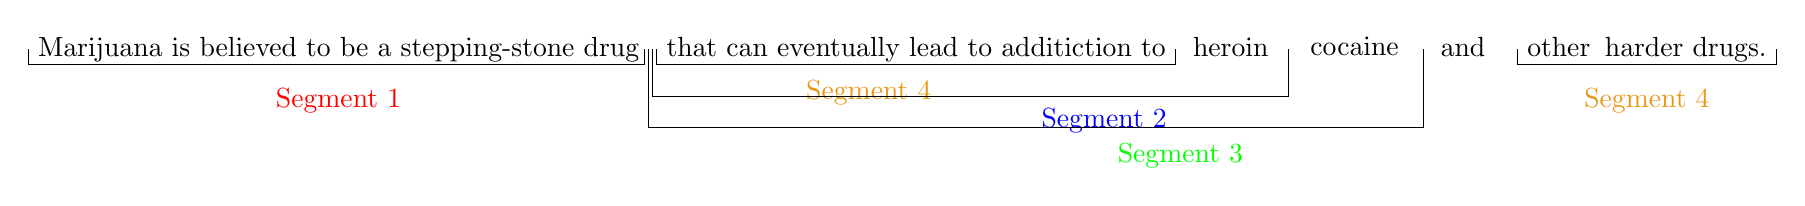
\begin{tikzpicture}[node distance=1mm]
\node (s1) {Marijuana is believed to be a stepping-stone drug};
\node (s234) [right=of s1]{that can eventually lead to additiction to};
	\node (s2) [right=of s234]{heroin\textcolor{white}{y}};
	\node (s3) [right=of s2.east]{cocaine\textcolor{white}{y}};
	\node (o) [right=of s3] {and\textcolor{white}{y}};
	\node (s4) [right=of o] {other\textcolor{white}{y}harder drugs.};

\node (s1lab) [below=of s1] {\textcolor{red}{Segment 1}};
\node (s2lab) [below=of s2, xshift=-1.7cm, yshift=-2.5mm] {\textcolor{blue}{Segment 2}};
\node (s3lab) [below left=1cm of s3, xshift=1mm, yshift=-1mm] {\textcolor{green}{Segment 3}};
\node (s4lab1) [below=of s234, xshift=-0.6cm, yshift=1mm] {\textcolor{orangegreen}{Segment 4}};
\node (s4lab2) [below=of s4] {\textcolor{orangegreen}{Segment 4}};

\draw [-]
($(s1.east) - (0.5mm, 0)$)
-- ++(0, -.2)
-| ($(s1.west) $);

% S4 segment
\draw [-]
($(s234.east) $)
-- ++(0, -0.2)
-| ($(s234.west) - (0, 0) $);

% S2 segment
\draw [-]
($(s234.west) - (0.5mm, 0)$)
-- ++(0, -0.6)
	-| ($(s2.east) - (0.5mm, 0) $);

% S3 segment
\draw [-]
($(s234.west) - (1mm, 0)$)
-- ++(0, -1.0)
-| ($(s3.east) $);

% other S4 segment
\draw [-]
($(s4.west) $)
-- ++(0, -.2)
-| ($(s4.east) $);
\end{tikzpicture}
	\caption{An example of comment made in the ``Marijuana'' topic. 
	\textcolor{red}{Claim 1} is a regular segment. 
	\textcolor{blue}{Claim 2} and \textcolor{green}{Claim 3} are mutually overlapping.
	\textcolor{orangegreen}{Claim 4} is both overlapping and discontiguous.}
	\label{fig:segment_example_range}
\end{figure}

%'<S1>Marijuana is believed to be a stepping-stone drug
%</S1><S2><S3><S4>that can eventually lead to addiction to
%</S3></S4>heroin,</S2><S3> cocaine</S3> and<S4> other harder
%drugs.</S4>'

% <S1>Nothing can bring peace to this earth.</S1> <S2>Its a great idea to try and
% push for world peace</S2> <S3>but it will never happen...</S3>'

\begin{algorithm}[t]
	\begin{algorithmic}[1]
\Function{is\_punctuation}{ch}
		\If{$ch = ``." \hspace{0.1cm} \cup \hspace{0.1cm} ch = ``?"
		\hspace{0.1cm} \cup \hspace{0.1cm}  ch = ``!"$}
\State
\Return $\mathit{True}$
\Else
\State
\Return $\mathit{False}$
\EndIf
%\Return $out$
\EndFunction

\State
\State 

\Function{na\"ive\_heuristic}{$text$}

	\State $\mathit{seg\_id} \gets 1$
	\State $Y[\mathit{seg\_id}] \gets \emptyset$
	\ForAll{$i \in |\mathit{text}|$}
		\State $token \gets text[i]$
		\State $Y[\mathit{seg\_id}] \gets Y[\mathit{seg\_id}] \cup \mathit{token}$
		\State
		\If{$\mathit{IS\_PUNCTUATION}(\mathit{token}) \cap i \neq 0$}
		\State $\mathit{seg\_id} \gets \mathit{seg\_id} + 1$
		\EndIf
	\EndFor
	\State
	\Return $Y$
\EndFunction
\end{algorithmic}
\caption{Claim segmentation punctuation based heuristic.
Input is a list of tokens, outputs a nested list of lists, where 
each list corresponds to a segment. 
None of the tokens is declared as non-argumentative.
The \texttt{IS\_PUNCTUATION} function has been simplified for readability
purposes, since in practice it uses regular expressions. 
	}
\label{alg:heuristic_claimseg}
\end{algorithm}

\section{Models}
\label{sec:claim_seg_model}

We frame the claim segmentation problem as supervised learning token-level 
classification (as it was done in \citep{ajjour2017unit} to detect
argumentative units of text). 
To label tokens, we use one of two 
token-level tagging solutions. 
First, we adopt the binary relevance multi-label classification (\texttt{BR})
approach, where each token can belong to zero or more claim segments. For the
second (\texttt{BIO}) approach, we discard overlapping and discontiguous
segments and then apply standard \texttt{BIO} labels.  After applying the
tagging to data, we propose three models to solve the claim segmentation
problem. In the first we apply a classic approach from argumentation mining
literature where each sentence is treated as a claim segment. For the second approach 
we use n-gram features as input to a SVM. In the third and last approach
we combine deep learning and structured prediction.

\paragraph{Na\"ive Heuristic. } 
Our baseline model is extremely similar to most approaches in argumentation
mining: we declare each sentence of the comment to be a claim.  This approach
is common in argumentation mining with the difference that some sentences may
be non-argumentative \citep{rooney2012applying,
stab2014identifying}.  We consider our assumption is reasonable, given
that a large portion (>80\%) of the dataset is argumentative.  For each
comment, we simply iterate through all tokens and start a new claim when a
token equals a punctuation mark.  This is a similar to sentence segmentation
\citep{palmer2000tokenisation}.  The heuristic is outlined in
algorithm~\ref{alg:heuristic_claimseg}.  An example of how the algorithm works
for a comment is shown in table~\ref{tab:heuristic_example}. This approach
inherently can not extract discontiguous and overlapping segments.

\begin{table}[t]
\begin{tabular}{@{}p{0.5\linewidth} p{0.50\linewidth}}
\toprule
\multirow{7}{*}{
\parbox{7cm}{
\textit{if we legalize pot there wil be a sharp increase in 
demand and consumption over a period of time
then............it will start to decline....slowly at first until
smoking pot becomes drinking wine.......only on special
occasions........... that's why we should continue the war
it's not like weed is damn near impossible to obtain ...... in my
opinion there is no war ....... there never was ...}
}}
		& \emph{if we legalize pot there wil be a sharp increase in 
demand and consumption over a period of time
	then ............} \\ \cline{2-2}
		& \emph{it will start to decline .... } \\ \cline{2-2}
		& \emph{slowly at first until
	smoking pot becomes drinking wine .......} \\  \cline{2-2} 
	& \emph{
only on special
occasions
...........
		} \\  \cline{2-2}
	& \emph{
that's why we should continue the war
it's not like weed is damn near impossible to obtain ......
		} \\\cline{2-2}
	& \emph{
in my
opinion there is no war .......
} \\\cline{2-2}
	& \emph{
there never was ...
} \\
\bottomrule
\caption{Example of heuristic algorithm output. }
\label{tab:heuristic_example}
\end{tabular}
\end{table}

\paragraph{SVM. } 
We use a weighted SVM. 
Class weights compensate for the disbalance amongst classes. 
The ratio between classes in the training set is used to set weight values, 
with the intent being in 
giving classes with less examples more prominence. 
% # We use the token and a configurable-sized context window of surrounding tokens
% # as input to the model. 
For features, we use tf-idf and 
distributed word representations 
(fastText\footnote{https://fasttext.cc/}
and word2vec\footnote{https://code.google.com/archive/p/word2vec/}
pretrained vectors).
Finally, to train the model, we use $5 \times 3$ nested-cross validation
optimizing hyperparameters $C$ and $\gamma$ using
grid-search (model selection described in section~\ref{sec:selection}).

\paragraph{BiLSTM+CRF Model.}
Finally, we try combining deep learning (BiLSTM) and structured prediction
(CRF).  The reason we opt for this model is two fold. First, BiLSTMs have
previously been successfully used in argumentation mining
\citep{habernal2016argument}.  Second, the combination of a BiLSTM with a CRF
is considered an extremely strong baseline (and often proves as a topline) for
sequence tagging problems \citep{huang2015bidirectional}.  The general idea of
a BiLSTM+CRF model is described in subsection~\ref{subsec:lstm_crf}.  We make a
few minor modifications in our model.  Our model works in two stages. In the
first stage, a BiLSTM is used to encode a sequence of tokens of the comment.
The BiLSTM produces pairs of hidden states and outputs. The outputs of the
BiLSTM are then fed into a feed-forward linear layer which maps the BiLSTM
outputs to the label probability space. In the second stage, the output of the
BiLSTM is used as features for the CRF.  The CRF combines the BiLSTM outputs
with a state transition table of possible tags to efficiently use past and
future tags to predict the current tag. The Viterbi algorithm (described in
subsection~\ref{sec:viterbi}) is used to efficiently compute optimal tag
sequences. 

The parameters of the BiLSTM+CRF model include 
\begin{enumerate*}[label=(\arabic*)]
\item BiLSTM parameters, 
\item linear layer weights, and 
\item state transition matrix of the CRF. 
\end{enumerate*}
As for the hyperparameters of the model, we use 200 feed forward units, set the
word embedding size to 300, and use a single layer bi-directional LSTM to encode
sequences.  We consider using pretrained word embeddings and training
embeddings from scratch.  Furthermore, we experiment by enabling and disabling
fine-tuning of input embeddings when using pretrained word embeddings.  
We use negative log likelihood as the loss function. We train
and evaluate the model using 5-fold cross-validation. 

% potencijalno staviti u experiments
%  When experimenting with In the multi-label
%  setup, we attempt to share the transition matrix across different when training
%  across claims.  

\section{Experiments}
\label{sec:claim_seg_experiment}

\begin{algorithm}[t]
\begin{algorithmic}[1]
	\Function{precision\_offset}{$\mathit{predicted}, \mathit{true}, \mathit{offset}$}
\State $\mathit{found} \gets \{\}$
\State
\ForAll{$i \in |\mathit{true}|$}
  \ForAll{$j \in |\mathit{predicted}|$}
	\State $\mathit{common} \gets $\texttt{LCS\_LENGTH}$(\mathit{true}[i], \mathit{predicted}[j])$
	\State
	\State $\mathit{is\_smaller\_than\_offset} \gets |\mathit{predicted}[j]| > \mathit{offset}$
	\State $\mathit{is\_common\_enough} \gets $ $|\mathit{predicted}[j]| -
	\mathit{common} \leq \mathit{offset}$
	\State $\mathit{has\_small\_size\_diff} \gets |\mathit{predicted}[j]| -
	|\mathit{true}[i]| \leq \mathit{offset}$
	\State
	\If{$\mathit{is\_smaller\_than\_offset} \cap 
	\mathit{is\_common\_enough} \cap \mathit{has\_small\_size\_diff}$}
	  \State $\mathit{found} \gets \mathit{found} \cup \mathit{true}[i]$
	  \State \textbf{break}
	\EndIf
  \EndFor
\EndFor
\State 
\State
\Return $\frac{|found|}{|true|}$
\State
\EndFunction
\end{algorithmic}
\caption{Algorithm to calculate precision with arbitrary offset between 
	two sets of segments, each segment being a list of tokens.
	\texttt{LCS\_LENGTH} calculates the length of the 
	longest common subsequence of two sequences.  
	We use a solution presented in
	\citep{hunt1977fast}.
	Recall is equivalently calculated, but with different inputs. 
	}
\label{alg:precision_offset}
\end{algorithm}

We compare the models using two main set of metrics. The first set of 
metrics is standard when evaluating information extraction problems:
 precision, recall, and F1-score of the retrieved claims, 
which we denote with P, R and F1 respectively. 
Also, since we're dealing with sequences, we wish to allow 
for small mistakes. This means that a retrieved claim which
has an extra or missing token will still count as correctly retrieved. 
Algorithm~\ref{alg:precision_offset} shows how to calculate precision with an
configurable margin of error (offset) on the token level.
The measure indicates when the predicted claim is close to the gold one,
since having exact claims might not always be important. For example, the
comment ``\emph{Nothing can bring peace to this earth. Its a great idea to try and
push for world peace, but it will never happen...}'' contains three claims,
one of them being ``\emph{but it will never happen...}'', but if the predicted claim is
``\textit{world peace but it will never happen...} and the allowed offset is two or more
this will be counted as correct. We can even see that in this example it might be useful 
to have additional information in the claim since it provides additional 
context.
The reported results use allowed offset of two and denote precision,
recall, and F1-score with offset as oP, oR, and oF1 respectively.

\begin{table}
	\centering
\begingroup
\setlength{\tabcolsep}{10pt} % Default value: 6pt
\renewcommand{\arraystretch}{1.5} % Default value: 1
	\begin{tabular}{l c  c c c c c c}
\toprule
		Tagset & Model & P & R & F1 & oP & oR & oF1 \\
      \midrule
		& Heuristic    & \textbf{0.41} & 0.23 & 0.29 & 0.89 & 0.49 & 0.63 \\
		\cline{2-8}
		\multirow{2}{*}{\texttt{BR} } & SVM & 0.03 & 0.01 & 0.02 & 0.09 & 0.01 & 0.02 \\
		                     & BiLSTM + CRF & 0.12 & 0.01 & 0.02 & 0.32 & 0.04 & 0.06 \\
		\cline{2-8}
		\multirow{2}{*}{\texttt{BIO}} & SVM & 0.35 & 0.14 & 0.20 & 0.88 & 0.35 & 0.50 \\
				     & BiLSTM + CRF & 
				     \textbf{0.41} & 
				     \textbf{0.27}  & \textbf{0.32} & \textbf{0.92} & \textbf{0.61} & \textbf{0.74} \\
      \bottomrule
	\end{tabular}
	\endgroup
	\caption{Claim segmentation standard and offset (set to two) precision, recall, 
	and F1 score in the \texttt{BR} and \texttt{BIO} setups. }
	\label{tab:claim_seg_results}
\end{table}

\paragraph{Multi-label encoding (\texttt{BR}).} 
First, we wish to compare the three proposed approaches: 
the na\"ive heuristic, the SVM, and the BiLSTM+CRF
in terms of both standard and offset precision, recall, and F1-score.
In both the SVM and BiLSTM+CRF approach, we use \texttt{BR} encoding. 
In the CRF, we don't share the tag transition table across 
claim segments and train embeddings from scratch.
Results are in table~\ref{tab:claim_seg_results} with boldfaced
best results. 
The results clearly show that the na\"ive heuristic model significantly outperforms
both the BiLSTM+CRF and the SVM model using \texttt{BR} encoding. 
The results of the heuristic model have
high precision and low recall. One reason may be that 
the model favors longer claims segments (that map to sentences). 
Intuitively, longer sentences contain more claims, on which the 
heuristic model performed poorly. 
By inspecting the outputs of the SVM and BiLSTM+CRF model, they consisted of
mainly majority class labels, so they manage to extract claims in short posts
(consisting of very claims). 
An obvious problem for the SVM and BiLSTM+CRF model 
is not having enough data points  
(100 samples for 48 labels). We considered reusing data across different
labels, but to no significant effect, since most of the training examples were
then labeled differently. More specifically, it would often be the case that
a token would be labelled as a claim in one
training instance, but not in another.
This is a less of a problem when dealing with a task such as named entity
recognition, as the number of such conflicting data points is much smaller. 
This clearly suggests that using the \texttt{BR} encoding struggles to 
predict claims. 
To improve the results, we also attempt to fine tune pretrained embeddings
during training time and share the transition table in the BiLSTM+CRF setup. 
Sharing the CRF
state transiton table  (which in this case defines the probability of going from a
non-argumentative to an argumentative state and vice versa) across folds should provide
models stronger priors of when a claim starts or ends. 
However, we do not see any performance improvement in that case either.

\paragraph{\texttt{\textbf{BIO}} encoding.} 
Since using \texttt{BR} encoding produces limited results 
even with the contiguous and non-overlapping claims, we explore the
\texttt{BIO} encoding. In order to do so, we first need to label the
dataset using \texttt{BIO} tags. Before applying the \texttt{BIO} tagset, overlapping
and discontiguous claims are discarded. Then, we assign \texttt{BIO} tags
to tokens (example in \texttt{BIO} labeling is shown in
Fig.~\ref{fig:segment_example_bio_multi-label}). 
To measure the topline results, we perform the inverse mapping from \texttt{BIO} tags
to claims and compare against gold claims (which include discontiguous and overlapping 
claims).
The topline precision, recall, and F1-score are then $1.0$, $0.74$, and $0.84$
respectively. Using the token and \texttt{BIO} tag pairs, we now train the
SVM and BiLSTM+CRF models.  This time around, we end up with comparable results
with the na\"ive heuristic baseline, as shown in the final two rows of
table~\ref{tab:claim_seg_results}.  
The SVM model performs 0.09 and 0.13 less F1-score percentage points than the
na\"ive heuristic, but much better (0.32 and 0.79 more F1-score percentage
points) than the SVM model using \texttt{BR} encoding. 
In terms of F1-score, the BiLSTM+CRF showed the best performance, narrowly
outperforming the na\"ive heuristic by 0.03 and 0.09 F1-score percentage points. 
% The na\"ive heuristic has higher precision, most likely since it produced less
% claim segments (509 versus 565 by the BiLSTM+SVM model). 

Looking at the results in general, predicting the exact boundary of a  claim
segment is a difficult task, since the best performing model produced
0.32 F1-score. 
However, the claims produced were often very close to the exactly correct one, 
which is reflected with the 0.74 offset F1-score for the best-performing model. 
Inspecting the predicted labels of all models, none of the models
correctly label non-argumentative segments (\texttt{O} labels). 
The most likely reason lies in the fact that non-argumentative content
is greatly underrepresented in this dataset and we should work on a method to 
such as penalizing or oversampling. 
In general, to solve the claim segmentation problem, the na\"ive
heuristic proved difficult to beat, even by advanced deep learning and
structured prediction techniques.
To further research on claim segmentation, we propose working on slighly more
advanced heuristics as a starting point, as a very simple one produced decent
results. The claim segmentation looks like mostly a syntax-related problem, so
perhaps looking into exploiting syntactic clues would yield even better
results.  In chapter~\ref{chap:claim_structuring}, we will revisit claim
segmentation as part of a joint model that also structures claims. 

% Now that we
% have scratched the  claim segmentation problem, we move on to the
% next stage in the argumentation mining pipeline: argumentative structure
% prediction. 
% 
% 110 # precision basic 208 509 0.4086444007858546                                                                                                                                                                   
% 111 # recall basic 208 921 0.2258414766558089                                                                                                                                                                      
% 112 # offset 452 509 0.888015717092338                                                                                                                                                                             
% 113 # offset 452 921 0.49077090119435396                                                                                                                                                                           

% # separate classifiers, non shared transitions
% # precision basic 31 288 
% # recall basic 30 921
% 
% # joined classifiers, non shared transitions
% # precision basic 28 203
% # recall basic 27 921

% BiLSTM with adam
% precision basic 251 614 0.40879478827361565
% recall basic 251 921 0.2725298588490771
% offset 565 614 0.9201954397394136
% offset 565 921 0.6134636264929425


% BiLSTM with offset
% # basic 254 641
% # basic 254 921
% # offset 528 838
% # offset 528 921
% 
% # epoch = 25
% # precision 204 / 641
% # recall 204 921



% # SVM BR
% # precision basic 3 99 0.030303030303030304
% # recall basic 3 921 0.003257328990228013
% # offset 9 99 0.09090909090909091
% # offset 9 921 0.009771986970684038

% # SVM BIO
% # precision basic 129 365 0.35342465753424657
% # recall basic 129 918 0.14052287581699346
% # offset 322 365 0.8821917808219178
% # offset 322 918 0.35076252723311546

% \section{Conclusion}
% \label{sec:claim_seg_conclusion}

% In this chapter, we have explored the claim segmentation problem.  We
% constructed a dataset of comments split into claims. The claim segmentation
% problem was then mathematically formalized in two ways: a multi-label
% binary relevance and a \texttt{BIO} encoding setup. The comparison of a
% na\"ive heuristic, SVM, and BiLSTM+CRF model 
% showed that a simple sentence splitting heuristic is a strong baseline to
% detect claims in text. This justifies the approach of most argumentation
% mining literature which assumes claims matches very well to sentences. 
% Additionally, trying to detect discontiguous and overlapping claims proved 
% extremely difficult in all experimental setups. 
% Perhaps starting from a purely structured SVM
% approach proposed by \citet{mcdonald2005flexible} would yield better results.



% microstructure vs. ontologies
\chapter{Formalizing claims}

This chapter is about formalizing claims. \\
this should contain the microstructure approach and the ontology approach \\

\section{Microstructures}

\begin{figure}
	\begin{center}
      \includegraphics[scale=1]{microstructure.pdf}
      \end{center}
      \caption{Claim microstructure (2nd-order).}
  \label{fig:structures_flowchart}
\end{figure}

- microstructures are structures expressing relations between the domain-specific
concepts, reflecting beliefs, value judgements, or desired policies of the claim
author \\
- their purpose is to capture the gist of the claim \\
- they stemmed from as many claims could be expressed as a \emph{relation} between \emph{concepts} using 
a certain \emph{modality} \\
- figure~\ref{fig:structures_flowchart} shows a claim microstructure bringing three elements 
together \\

\noindent - Relations.  \\
- Many claims can be represented as expressing a relation between two concepts \\
- for example, on the topic of ``Gay Rights'' , the relations may be 
`\texttt{promotes(gay marriage, depopulation)}' and 
`\texttt{purpose(love, procreation)}' \\
- there are also comparably fewer claims that can be expressed via
higher-order relations , e.g. `\texttt{entails(constitution, allow(state, gay marriage))} \\
- each relation can be negated, e.g. $\neg$\texttt{promotes(gay marriage, depopulation)} expresses
that gay marriage does not cause depopulation \\
- relations are domain independent \\

\noindent Concepts \\
- the relations are established between concepts, expressed by noun phrases \\
- for ease of access, they can be arranged into a small, domain specific taxonomy of concepts \\
- for instance ``gay marriage'', ``heterosexual marriage'' and ``religious marriage''
all belong under the concept of ``marrriage'' \\
- the taxonomic relations could also be useful for later computational processing \\
- concepts are domain dependent and need to defined for each topic anew \\

\noindent Modalities \\
- we observe that claims are expressed under different modalities \\
- they can be roughly categorized into \textit{beliefs, value judgements, and policies} \\
- we formalize this via unary relations `believes', `approves', `disapproves', and `desires' corresponding 
to beliefs (factual, religous, and opinion-based), positive value judgements, negative value 
judgements, and desired policy (desired state of affairs) respectively \\
- the three modalities act as a wrapper on the propositional content of the claim, 
effectively modulating what is being claimed \\
- for instance, `\texttt{believes(purpose(love, procreation))}' expresses the belief 
that love serves procreation, while \texttt{desires(}$\neg$\texttt{allow(state, gay marriage))}'
expresses the wish for the state not to allow gay marriages \\
- finally, in a number of claims the claim is expressed with a reference to a second
opinion holder (e.g. the Bible, the state) \\
- to tackle this, we add an additional modality layer with the opinion holder as
an additional modifier \\
- for instance `\texttt{believes(believes[state](promotes(marriage, advancement)))}' corresponds
to the belief that the state believes gay marriages lead to an advancement \\
- by convention , the opinion holder of the first modality is always the author of the post \\

\begin{table}
{\footnotesize
\begin{tabular}{lp{0.80\columnwidth}}
\toprule
\textbf{Relation} & \textbf{Definition} \\
\midrule
\texttt{promotes(A, B)} & Promoting agent A promotes, fosters, leads, increases likelihood, boosts B.  \\
\texttt{suppress(A, B)} & Suppressing agent A suppresses, decreases likelihood, puts down, vanquishes B \\
\midrule
\texttt{allow(A, B)} & Principle A allows, approves, licenses state of affairs B \\
\midrule
\texttt{entails(A, B)} & State of affairs A, necessarily, per definition or causally, makes B true. \\
\texttt{contradicts(A, B)} & State of affairs A, necessarily, per definition or causally, makes B false. \\
\midrule
\texttt{purpose(A, B)} & The purpose of A is B. \\
\midrule
\texttt{equal(A, B)} & State of affairs A is equal to state of affairs B. \\
\midrule
\texttt{has(A, B)} & A has the properties affected by the existence of B.  \\
\bottomrule
\end{tabular}}
\caption{Relation types in claim microstructures.}
\label{tab:microstructures_relations}
\end{table}

\noindent - $\mathcal{R}, \mathcal{C}$, and $\mathcal{M}$ denote the set of relations, concepts and
modalities, respectively \\
- we define a claim microstructure as a quadruple 
$$
(m_1, m_2, o_2, r)
$$ 
where $m_1 \in \mathcal{M}$, and (optionally) $m_2 \in \mathcal{M} \cup \{\epsilon\}$,
$o_2 \in \mathcal{C} \cup \{\epsilon\}$ is the optional second opinion holder, and 
$r = (t, c_1, c_2) \in \mathcal{R}$ is the (possibly higher order) relation 
between two concepts or relations $c_1, c_2 \in \mathcal{C} \cup \mathcal{R}$, 
conveyed by the relation type $t$. \\
- table~\ref{tab:microstructures_relations} lists all possible relation types \\


\chapter{Claim Structuring}
\label{chap:claim_structuring}

In the previous chapter, we have introduced two main approaches defining claim
formalizations.  Having formalized claims can help in deriving inferred claims
or help with related downstream tasks (such as stance classification) as it
will be shown in chapter~\ref{chap:analysis}.
Formalized claims can be obtained manually, applying the steps laid out in the 
claim ontology framework in chapter~\ref{chap:formalization}. 
In this chapter, we wish to explore how some of the steps of the framework can 
be automatized: formalizing new claims when the rest of the framework is already setup.
In a setting where the domain ontology has been determined (domain is
restricted and closed) we wish to explore how feasible it is to automatically
acquire formalized claims from raw text claims: solve the \textbf{claim structuring}
problem.

First, we introduce the dataset which will be used for claim structuring
in section~\ref{sec:claim_struc_data}. Then we define models that attempt to solve the 
claim structuring problem in section~\ref{sec:claim_struc_models}. 
The models are applied to the data in multiple setups in section~\ref{sec:claim_struc_experiment}.
We conclude in section~\ref{sec:claim_struc_conclusion}. 

\section{Data}
\label{sec:claim_struc_data}

We export the ontology designed in 
% TODO add reference
section. 
% TODO check numbers
The ontology contains a total of 920 claims. Out of those 920, three annotators 
A1, A2, and A3 manage to formalize X, Y, and Z respectively.
We take formalizations from annotator A1. 
Next, we attempt to formulate claim structuring as a supervised learning problem. 
Two basic approaches are considered: predicting components of the formalization then putting
them together (\emph{molecule}) or predicting the entire formalization (\emph{atomic}). 
Using components corresponds to a more realistic scenario, as it more
faithfully reflects how the claim formalization is built manually. 

Following the molecule approach, the formalized ontology claim can be broken
down into four main components:
\begin{itemize}
	% TODO add mathematical notation from ontology section
	\item \emph{modality} ($\mathit{MOD} \in \{\mathit{fact},
		\mathit{good value}, \mathit{bad value}, \mathit{policy}\}$), 
	\item \emph{count} ($\mathit{CNT} \in \{\mathit{unary},
		\mathit{binary},  \mathit{ternary}\}$),
	\item \emph{properties} ($\mathit{PR} \in \{\mathit{has\_antecedent},
		\mathit{has\_declaration}, \mathit{implies}, \dots\}$)
	\item \emph{domain individuals} ($\mathit{DI} \in \{\mathit{marijuana},
		\mathit{legalized\_marijuana}, \mathit{mafia\_bankrupt},
		\dots\}$)
\end{itemize}
Now, to construct a formalized claim, we use a exactly one (out of four
possible) \emph{modality}, exactly one (out of three possible) \emph{count},
one or more (up to three, out of 22 possible) \emph{properties}, and one
or more (out of 82 possible) \emph{domain individuals} (one for each property). 
We could have had negation as an extra component of the formalized claim, but
since only properties may be negated, we construct the properties set $P$ as a
union of properties and their negations: 
$$
P = \{\mathit{has\_antecedent}, 
\mathit{negated\_has\_antecedent}, \mathit{implies}, \mathit{not\_implies}\, \dots\}
$$

Taking into consideration all possible combinations of components from
annotator A1, 106 binary labels ($82 \cdot \mathit{DI} + 17 \cdot \mathit{PR} + 4\cdot
\mathit{CNT} + 3 \cdot \mathit{MOD}$) can be assigned to a claim, from which a
formalized claim can be constructed.  This means that there  exists an
exponential ($2^{106}$) number of possible formalizations, a large number of
which is invalid.  An invalid formalization example would involve both
\texttt{has\_declaration} and \texttt{has\_antecedent} which is not allowed,
since \texttt{has\_declaration} can only be assigned to a \texttt{unary} claim,
whereas \texttt{has\_antecedent} can only be assigned to \texttt{binary} claim. 

\begin{figure}
	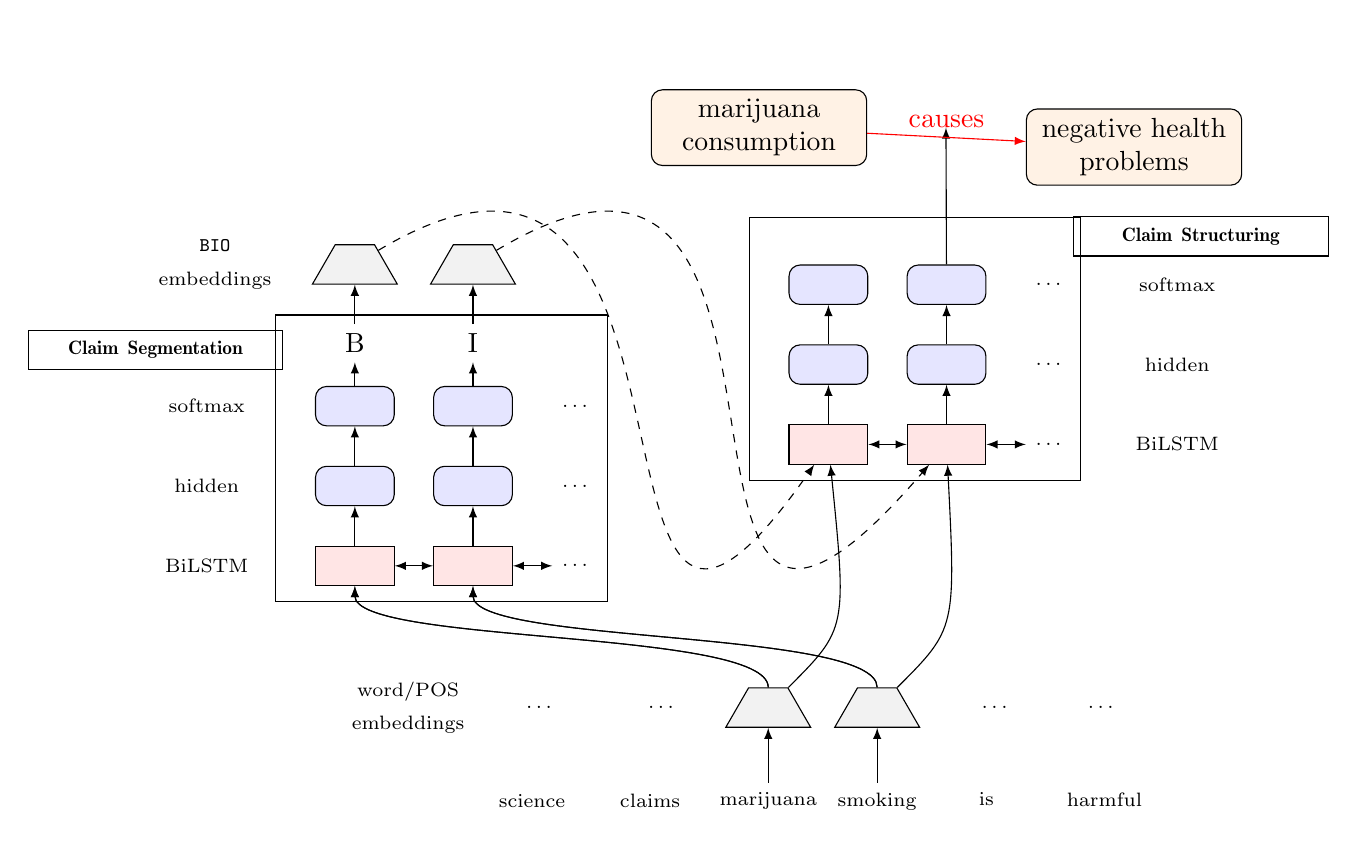
\begin{tikzpicture}[node distance=1.5cm]
\tikzstyle{lstm} = 
[rectangle, minimum width=1cm, minimum height=0.5cm, text
centered, draw=black, fill=red!10]
\tikzstyle{hidden} = 
[rectangle, minimum width=1cm, minimum height=0.5cm, text 
centered, draw=black, fill=blue!10, rounded corners]
\tikzstyle{embed} = 
[trapezium, minimum width=1cm, minimum height=0.5cm, text 
centered, draw=black, fill=gray!10]
\tikzstyle{label} = 
[minimum width=1cm, minimum height=0.5cm, text 
centered, text width=1.5cm]
\tikzstyle{dots} = 
[minimum width=0.3cm, 
minimum height=0.5cm, text 
centered, text width=0.3cm]
\tikzstyle{component} = 
[minimum width=1cm, minimum height=0.5cm, text 
centered, text width=3cm, rectangle, draw=black]
\tikzstyle{concept} =
[rectangle, minimum width=1cm, minimum height=0.5cm, text 
centered, draw=black, fill=orange!10, rounded corners, text width=2.5cm]

\node (lstm_1) [lstm] {};
\node (lstm_2) [lstm, right of=lstm_1] {};
\node (dots_1) [dots, right=0.5cm of lstm_2] {\scriptsize{\dots}};
\node (hidden_1) [hidden, above=0.5cm of lstm_1] {};
\node (hidden_2) [hidden, above=0.5cm of lstm_2] {};
\node (dots_2) [dots, right=0.5cm of hidden_2] {\scriptsize{\dots}};

\node (hidden_3) [hidden, above=0.5cm of hidden_1] {};
\node (hidden_4) [hidden, above=0.5cm of hidden_2] {};
\node (dots_3) [dots, right=0.5cm of hidden_4] {\scriptsize{\dots}};

\node (B_lab) [above=0.3cm of hidden_3] {B};
\node (I_lab) [above=0.3cm of hidden_4] {I};

\node (trapez_1) [embed, above=0.5 cm of B_lab] {};
\node (trapez_2) [embed, above=0.5 cm of I_lab] {};

\draw ($(hidden_3.north west) + (-0.5, 0.9)$) rectangle ($(lstm_2.south east) + (1.2, -0.2)$);

\node (word_1) [below right=2.5cm and 4cm of lstm_1] {\scriptsize{marijuana}};
\node (word_2) [below right=2.5cm and 4cm of lstm_2] {\scriptsize{smoking}};
\node (word_3) [right of=word_2] {\scriptsize{is\textcolor{white}{jg}}};
\node (word_4) [right of=word_3] {\scriptsize{harmful\textcolor{white}{jg}}};
% \node (word_0) [left of=word_1] {\scriptsize{\dots}};
% \node (word_5) [right of=word_4] {\scriptsize{\dots}};
\node (word_m1) [left of=word_1] {\scriptsize{claims}};
\node (word_m2) [left of=word_m1] {\scriptsize{science}};

\node (w_1) [embed, above=0.7cm of word_1] {};
\node (w_2) [embed, above=0.7cm of word_2] {};
\node (dots_word1) [dots, right=0.8cm of w_2] {\scriptsize{\dots}};
\node (dots_word4) [dots, right=0.8cm of dots_word1] {\scriptsize{\dots}};
\node (dots_word2) [dots, left=0.7cm of w_1] {\scriptsize{\dots}};
\node (dots_word3) [dots, left=1cm of dots_word2] {\scriptsize{\dots}};

\node (lstm_3) [lstm, above right=-1 cm and 3.5cm of hidden_4] {};
\node (lstm_4) [lstm, right of=lstm_3] {};
\node (hidden_5) [hidden, above=0.5cm of lstm_3] {};
\node (hidden_6) [hidden, above=0.5cm of lstm_4] {};
\node (hidden_7) [hidden, above=0.5cm of hidden_5] {};
\node (hidden_8) [hidden, above=0.5cm of hidden_6] {};
\node (lstm2_dots_1) [dots, right=0.5cm of lstm_4] {\scriptsize{\dots}};
\node (lstm2_dots_2) [dots, right=0.5cm of hidden_6] {\scriptsize{\dots}};
\node (lstm2_dots_3) [dots, right=0.5cm of hidden_8] {\scriptsize{\dots}};

%\node (struc) [above=0.8cm of hidden_8] {};
\node (c_marijuana) [concept, above left=1.25 cm and 0.5cm of hidden_8] {marijuana consumption };
\node (c_health) [concept, above right=1cm and 0.5cm of hidden_8] {negative health problems};
\draw[-latex] (hidden_8) -- ($(c_marijuana.east) + (1, 0) $);

\draw[-latex, red] (c_marijuana) -- (c_health) node[midway, above] {causes};

\draw ($(hidden_7.north west) + (-0.5, 0.6)$) rectangle ($(lstm_4.south east) + (1.2, -0.2)$);
%\draw ($(hidden_7.north west) + (-0.3, 0.6)$) rectangle ($(lstm_4.south east) + (0.3, -0.6)$);
% 
% \node (lstm_5) [lstm, right=1 cm of lstm_4] {};
% \node (lstm_6) [lstm, right of=lstm_5] {};
% \node (hidden_9) [hidden, above=0.5cm of lstm_5] {};
% \node (hidden_10) [hidden, above=0.5cm of lstm_6] {};
% \node (hidden_11) [hidden, above=0.5cm of hidden_9] {};
% \node (hidden_12) [hidden, above=0.5cm of hidden_10] {};
% 
% \draw ($(hidden_11.north west) + (-0.3, 0.6)$) rectangle ($(lstm_6.south east) + (0.3, -0.6)$);
% 
% \node (lstm_7) [lstm, right=1 cm of lstm_6] {};
% \node (lstm_8) [lstm, right of=lstm_7] {};
% \node (hidden_13) [hidden, above=0.5cm of lstm_7   ] {};
% \node (hidden_14) [hidden, above=0.5cm of lstm_8   ] {};
% \node (hidden_15) [hidden, above=0.5cm of hidden_13] {};
% \node (hidden_16) [hidden, above=0.5cm of hidden_14] {};
% 
% \draw ($(hidden_15.north west) + (-0.3, 0.6)$) rectangle ($(lstm_8.south east) + (0.3, -0.6)$);

% labels of NN parts
\node (label_word_pos) [label, left=0.5cm of dots_word3] {\scriptsize{word/POS embeddings}};
\node (label_bilstm1) [label, left=0.5cm of lstm_1] {\scriptsize{BiLSTM}};
\node (label_hidden1) [label, left=0.5cm of hidden_1] {\scriptsize{hidden}};
\node (label_softmax1) [label, left=0.5cm of hidden_3] {\scriptsize{softmax}};
\node (bio_embeddings) [label, left=0.5cm of trapez_1] {\scriptsize{\texttt{BIO} embeddings}};

\node (label_bilstm1) [label, right=0.5cm of lstm2_dots_1] {\scriptsize{BiLSTM}};
\node (label_hidden1) [label, right=0.5cm of lstm2_dots_2] {\scriptsize{hidden}};
\node (label_softmax1) [label, right=0.5cm of lstm2_dots_3] {\scriptsize{softmax}};

%\node (label_bilstm2) [label, left=0.5cm of lstm_3] {\scriptsize{BiLSTM}};
%\node (label_hidden2) [label, left=0.5cm of hidden_] {\scriptsize{hidden}};
%\node (label_softmax2) [label, left=0.5cm of hidden_3] {\scriptsize{softmax}};

\node (bio_lstm) [component, above left=0.2cm and 0.4cm of hidden_3] 
{\scriptsize{\textbf{Claim Segmentation}}};

\node (struc_lstm) [component, above right=0.1cm and 1.1cm of hidden_8] 
{\scriptsize{\textbf{Claim Structuring}}};

%text width=4cm,minimum height=6cm,minimum width=10cm

% connections
% \draw[-latex] (trapez_1) .. controls +(up:1.5cm) and +(down:1cm) ..
% node[above, sloped] {} (lstm_3);
% \draw[-latex] (trapez_2) .. controls +(up:1.5cm) and +(down:1cm) ..
% node[above, sloped] {} (lstm_4);
% 
% \draw[-latex] (trapez_1) .. controls +(up:1.3cm) and +(down:2cm) ..
% node[above, sloped] {} (lstm_5);
% \draw[-latex] (trapez_2) .. controls +(up:1.3cm) and +(down:2.5cm) ..
% node[above, sloped] {} (lstm_6);
% 
% \draw[-latex] (trapez_1) .. controls +(up:1cm) and +(down:3cm) ..
% node[above, sloped] {} (lstm_7);
% \draw[-latex] (trapez_2) .. controls +(up:1cm) and +(down:3.5cm) ..
% node[above, sloped] {} (lstm_8);

% lstm connections
\draw[-latex] (lstm_1) -- (hidden_1);
\draw[-latex] (lstm_2) -- (hidden_2);
\draw[-latex] (hidden_1) -- (hidden_3);
\draw[-latex] (hidden_2) -- (hidden_4);
\draw[-latex] (hidden_3) -- (B_lab);
\draw[-latex] (hidden_4) -- (I_lab);

%\draw[-latex] (hidden_8) -- (struc);

% \draw[-latex] (lstm_1) .. controls +(up:1.1cm) and +(left:0.9cm) .. node[above, sloped] {} (lstm_2);
% \draw[-latex] (lstm_2) .. controls +(up:1.1cm) and +(left:0.7cm) .. node[above, sloped] {} (dots_1);

\draw[>=latex, <->] (lstm_1) -- (lstm_2);
\draw[>=latex, <->] (lstm_2) -- (dots_1);

\draw[>=latex, <->] (lstm_3) -- (lstm_4);
\draw[>=latex, <->] (lstm_4) -- (lstm2_dots_1);

\draw[-latex, dashed] (trapez_1) .. controls +(5cm, 3cm) and +(-3.5cm, -5cm) .. node[above, sloped] {} (lstm_3);
\draw[-latex, dashed] (trapez_2) .. controls +(5cm, 3cm) and +(-4.3cm, -5cm) .. node[above, sloped] {} (lstm_4);

\draw[-latex] (w_1) .. controls +(up:1cm) and +(down:1cm) .. node[above, sloped] {} (lstm_1);
\draw[-latex] (w_2) .. controls +(up:1cm) and +(down:1cm) .. node[above, sloped] {} (lstm_2);

\draw[-latex] (w_1) .. controls +(up:1cm) and +(down:1cm) .. node[above, sloped] {} (lstm_1);
\draw[-latex] (w_2) .. controls +(up:1cm) and +(down:1cm) .. node[above, sloped] {} (lstm_2);

\draw[-latex] (w_1) .. controls +(1cm, 1cm) .. node[above, sloped] {} (lstm_3);
\draw[-latex] (w_2) .. controls +(1cm, 1cm) .. node[above, sloped] {} (lstm_4);

%\draw[-latex] (w_1) -- (lstm_1);
%\draw[-latex] (w_2) -- (lstm_2);
\draw[-latex] (word_1) -- (w_1);
\draw[-latex] (word_2) -- (w_2);
\draw[-latex] (B_lab) -- (trapez_1);
\draw[-latex] (I_lab) -- (trapez_2);

\draw[-latex] (lstm_3) -- (hidden_5);
\draw[-latex] (lstm_4) -- (hidden_6);
\draw[-latex] (hidden_5) -- (hidden_7);
\draw[-latex] (hidden_6) -- (hidden_8);

\end{tikzpicture}


	\caption{Joint BiLSTM model for both claim segmentation and claim 
	structuring. }
	\label{fig:joint_model}
\end{figure}

\section{Models}
\label{sec:claim_struc_models}

We wish to build models for claim structuring. The models should produce 
formalized claims from text. 
Three model setups are proposed: independent classifiers, 
chain classification, and a joint model. 

\paragraph{Independent classifiers (IND). }
As a baseline approach, we use independent SVMs to predict components
For SVM features, we use distributed word representations
(fastText\footnote{https://fasttext.cc/}
and word2vec\footnote{https://code.google.com/archive/p/word2vec/}
pretrained vectors).
To train each independent model, we use $5 \times 3$ nested-cross validation.
We experiment with in both the \emph{atomic} and \emph{molecular} approach.

\paragraph{Chain classification (CC). }
To take advantage of formalization component dependencies, we adopt the chain
classification approach, as described in
section~\ref{sec:chain_classification}.
First, to verify this assumption we build a chain classifier which uses gold 
labels as input in each prediction.  
This yields performances of 
% TODO add performance
This promising performance is more than enough reason to adopt the
chain classification approach for claim formalization. 
We frame all component classifications as multilabel classification 
(generalizing even the multiclass count and modality prediction problems).
SVMs models are then chained such that the prediction of one SVM is added as
input to the following SVM model, until all labels are predicted. We randomize 
the ordering of labels which are predicted.
Additionally, to alleviate the influence of randomization, we 
ensemble chain classifiers (ECC) using a majority vote. 
It is sensible to use the chain classification model only in the
\emph{molecular} setting. 
To train the model, we use $5 \times 3$ nested-cross validation. 

\paragraph{Joint model (J). } 
Apart from dependencies in the claim structure, we wish to investigate whether
we can structure claims which aren't gold claims.  To that end, we present a
joint model which does claim segmentation (details described in
chapter~\ref{chap:claim_structuring}) and claim structuring in one step. We
draw inspiration from \citep{miwa2016end} where they use multiple consecutive
LSTM cells to predict multiple outputs.  We adopt a similar approach, where we
two sets of BiLSTM layers: first (\texttt{BiLSTM-seg}), to predict claims, and
second (\texttt{BiLSTM-struc}) to predict claim formalization components.  The
\texttt{BiLSTM-struc} layer is a shared, as we wish to update its parameters
when upon incorrect formalization in addition to incorrect claim segmentation.
The input of the \texttt{BiLSTM-seg} layer is a sequence of tokens and their
respective part-of-speech (POS) tags \citep{brown1957linguistic} paired \texttt{BIO}
tags (explained in section~\ref{sec:claim_seg_problem}). The output of the
\texttt{BiLSTM-seg} is a set of claims. Then each claim is formalized via the
\texttt{BiLSTM-struc}.  The model is outlined in figure~\ref{fig:joint_model}. 
We use three sets of embeddings: word, POS embeddings, and \texttt{BIO} tag
embeddings. The joint model is applied for both the \emph{molecular} and 
\emph{atomic} setup. 
% TODO add learning
We also experiment with both pretrained word embeddings. 

\section{Experiments}
\label{sec:claim_struc_experiment}

\begin{table}
	\centering
\renewcommand{\arraystretch}{2}%
	\begin{tabular}{p{3cm} c c c c  c  c c c  @{\hspace{1.5em}}c@{}  @{\hspace{1em}}c@{}  }
	\toprule
		\multirow{2}{*}{Model / Setup}
		& \multicolumn{2}{c}{\texttt{MOD}} 
		& \multicolumn{2}{c}{\texttt{CNT}} 
		& \multicolumn{2}{c}{\texttt{PR}}
		& \multicolumn{2}{c}{\texttt{DI}} 
		& \multicolumn{2}{c}{\texttt{CL}}
		\\

		& OR  & PA  & OR  & PA  & OR  & PA & OR  & PA &  OR & PA \\
		\midrule

		MAJ & & & & & & & & & & \\
		IND & & & & & & & & & & \\		
		CC & & & & & & & & & & \\
		ECC & & & & & & & & & & \\
		J-BiLSTM & & & & & & & & & & \\

		\bottomrule
	\end{tabular}
	\caption{F1-score comparison between 
	the independent SVM (IND), majority classifier (MAJ), chain classification (CC), 
	ensemble chain classification (ECC), and joint model (J)
	in the task of 
	claim structuring from both original (OR) and paraphrased text claims (PA)
	using the \emph{molecular} approach. 
	Results are compared on individual components
	across modalities \texttt{MOD}, counts (\texttt{CNT}), 
	properties (\texttt{PR}), and 
	domain individuals (\texttt{DI}). Finally, predictions are assembled into a 
	formalized claim and compared against the gold formalized claims (\texttt{CL}).
	}
	\label{tab:claim_struc_per_component}
\end{table}


We perform two sets of experiments. First, we wish to explore models
that predict the formalization structure on a per-component basis (structure
prediction). 
Second, we investigate  

\paragraph{Structure prediction feasibility. }
This approach is more realistic, as it would the number of possible
formalizations grows exponentially, we can expect the distribution of observed
formalizations is long tailed, therefore it is not feasible to expect to
predict infrequently seen formalizations.
Table~\ref{tab:claim_struc_per_component} shows macro averaged F1-scores for
the majority classifiers (MAJ), independent SVM classifiers (IND), chain
classifiers (CC), ensemble chain classifiers (ECC), and the joint segmentation
and structuring BiLSTM model (J-BiLSTM).  We experiment with both original
source claims (as they were written by the authors) and paraphrased claims (as
they were transcribed by annotators).
Models are trained to predict components, which are then assembled together to 
constitute a formalized claim, which is compared against the gold formalized claim. 
The baseline is set using the majority 
class , we use the majority class for all claim formalization individual 
components. 
The joint model might not produce the same number claim formalizations, 
so we evaluate on a post level and average across all posts. 
Additionally, we could have regularized the models by preventing invalid
formalizations perhaps in the form of constraint programming, but leave this
for future work. 

The results suggest that predicting components is a somewhat feasible tasks,
but predicting a correct combination of components seems very difficult.  The
most problematic proved predicting the correct property (\texttt{PR}), with
model X achieving the best performance of , which is still considered low. 
% TODO insert rest of comments on the results

% joint model analysis
In the joint model setup, we set the learning rate in all layers. 
We also experiment with setting lower learning rates for shared layers,
but to no significant performance boost. 
Looking into the joint model outputs, we notice that the formalization predictions
are particularly bad when predicted claims are far from sensible. 

\begin{table}
	\centering
%\renewcommand{\arraystretch}{2}%
	\begin{tabular}{p{3cm} c c c c }
	\toprule
		\multirow{2}{*}{Model / Setup}
		& \multicolumn{2}{c}{\texttt{AT}}
		& \multicolumn{2}{c}{\texttt{MO}}
		\\
		& OR  & PA  & OR  & PA \\
		\midrule

		MAJ & & & &  \\
		IND & & & & \\		
		J-BiLSTM & & & & \\

		\bottomrule
	\end{tabular}
	\caption{Claim segmentation
	F1-score using the 
	\emph{atomic} (\texttt{AT}) and \emph{molecular} (\texttt{MO})
	approach for original (OR) and paraphrased (PA) claims. 
	}
	\label{tab:claim_struc_atomic_molecular}
\end{table}

\paragraph{Expansion vs. structure prediction. } Even though the
\texttt{molecular} approach is more realistic setup, we explore now compare it
to the \texttt{atomic} setup, where we each claim formalization a label to 
train models to predict the claim. 
Results are listed in table~\ref{tab:claim_struc_atomic_molecular}.
% TODO compare results in general 
In general, if we compare the best \texttt{molecular} approach and
the best \texttt{atomic} approach \dots
% TODO compare results of assembly vs. 

All experiments clearly show that using paraphrases proved useful for
\textbf{all} approaches. This clearly suggests that claim paraphrases
proved useful for both claim understanding and for claim structuring. 
We hypothesize this is mostly due to the reduction of noisyness and 
vagueness of claims. 

% TODO some conclusion on the joint model vs. no joint model

\section{Conclusion}
\label{sec:claim_struc_conclusion}

We conclude that claim structuring is in general a difficult problem to solve, 
but with the help of structured approaches can achieve decent performance 
of X.
%TODO give some decent number .
Interestingly to note, results using paraphrased claims are significantly better across all 
models on average by F1-score points, which shows claim paraphrases make it
easier to process claims for both humans and machines (each in their own way). 
% TODO use paraphrased number - original average across all 

In the next chapter, we will explore the benefits of using formalized claims to
demonstrate the example argumentation analysis one can perform using formalized
claims. 



% analysis 
\chapter{Analysis using Formalized Claims}

This chapter is about using structured methods for argumentation mining
for claim analysis \\


\bookmarksetup{startatroot}
\addtocontents{toc}{\bigskip}% perhaps as well

\chapter{Conclusion}
\label{chap:conclusion}

% what was done -- summary
In the scope of doctoral thesis, we have researched multiple argumentation
mining problems in the domain of online discussions.  Argumentation mining
problems can be categorized according to where they lie in the argumentation
mining pipeline. The argumentation mining pipeline starts with text and
produces an argumentation structure. 
We worked on claim extraction, claim
structuring, and deriving implicit claims as part of our implementation of the
argumentation mining pipeline. To solve those problems, we make a distinction
between two approaches: an unstructured and a structured approach. In the
unstructured approach (part~\ref{part:unstruc}), we employ commonly-used machine
learning algorithms to extract natural language claims. On the other hand, in
the structured approach (part~\ref{part:struc}), we employ structured prediction
machine learning approaches. 
We opt for structured argumentation mining based on three pre-research studies
(described in chapters~\ref{chap:argclu}, \ref{chap:argrec}, and
\ref{chap:deriving_implicit}) which showed the limits of computational
representations of unstructured text. 

This work contains the following original scientific contribution. 
% Formalized claims
% (in comparison to natural language claims) contain a crisp logical
% representation of claims, which allows us to make inference to derive implied
% claims (chapter~\ref{chap:analysis}).

% reflection on contribution
This research proposes claim detection, structuring and analysis from online
discussions based on machine learning, natural language processing and
ontological modelling. Expected research contributions are: 1. Modeling an
online discussion using an two-level ontology, where the first level contains
domain knowledge and the second models claim patterns, aiming to fully
structure online discussions; 2. Supervised machine learning method for claim
detection and claim structuring; 3. Framework and support for online discussion
analysis involving claim detection, structuring, and analysis based on a
comparison of claims from all discussion participants


% future work, what more can be done in this area

% why is deriving implicit claims important
In general, we feel that deriving implicit claims is a very important, and
understated problem in not only argumentation mining, but also in computational
lingustics. To derive textual entailment, sentiment, In a recent news article,
the difficulty of acquiring implicit knowledge is highlighted
\citep{gradientpub}.  The news article criticizes the state-of-the-art language
model BERT \citep{devlin2018bert} to unravel that the state-of-the-art models
do not actually model implicit knowledge and human-level language
understanding, but exploit the statistical token-level cues often present in
datasets. We hope this research will inspire further research in argumentation
mining, in particular through exploring implicit claims and implicit knowledge. 


 
% \chapter{Datasets}

- my datasets \\

\section{ComArg}
- argrec dataset \\

\section{ArgPremises}
- argpremises dataset \\

\section{Microstructure}
- microstructure dataset \\

\section{Logical structures and ontology}
- logical structures ontology and dataset \\

\section{Related work of datasets}
\noindent - related work of argumentation mining datasets for each category \\
- related to argrec \\

\noindent - related to argpremises \\
- mention habernal semeval task \\

\noindent - related to microstructures dataset \\
- mention adam wyner's dataset \\

\noindent - logical structures and ontologies  \\
- computational argumentation datasets \\
- differences in relation to computational argumentation \\
- abstract argument vs. our argument \\


%%%%%%%%%%%%%%%%%%%%%%%% PRILOZI / APPENDIX %%%%%%%%%%%%%%%%%%%%%%%%%%%%%%%

%\appendix
%\addcontentsline{toc}{section}{Appendices}
%\renewcommand{\thechapter}{A}
%\renewcommand{\thesection}{\Alph{section}}
%\setcounter{section}{0}

%\begin{appendices}

\setcounter{chapter}{0}%
\renewcommand{\thechapter}{\Alph{chapter}}%  Letters as 'counters'
%\part{\appendixname}
\part{Appendices}

\chapter{Text Datasets}
\label{chap:appendix_datasets}

Here is the list of all the datasets created as part of this thesis.

\begin{enumerate}[label=\textbf{A.\arabic*}]
\item\label{item:comarg} \ComArg is a dataset of online user comments manually annotated with
comment-argument pairs. The dataset is created for the argument
recognition task: identifying what arguments, from a predefined
set of arguments, have been used in users' comments, and how.
It consists of 1285 and 1013 comment-argument pairs from 
on-line discussions of \emph{Gay Marriages} (GM) 
and \emph{Under God in pledge} (UGIP) respectively.
The dataset is publicly available at:
\url{http://takelab.fer.hr/data/comarg/}

\item\label{item:argpresmises} ArgPremises is a dataset of 
implicit premises manually annotated on matching claims. 
The dataset is created to explore what are the implied premises users 
make when expressing support for a claim.
Additionally, it was used to help solve the claim matching task; 
using implicit premise information whilst 
identifying whether a pair of claims expresses the same argument. 
It consists of 494 claim pairs and 3977 respective premises on topics
of \emph{Marijuana Legalization} (MA), \emph{Gay Rights} (GA), 
\emph{Abortion Legalization} (AB),
and \emph{Obama Presidency} (OB).
The dataset is publicly available at:
\url{http://takelab.fer.hr/data/argpremises/}

\item\label{item:microstructures_dataset} The Claim Microstructure dataset contains posts split into claim
segments, translated into claim microstructures. The dataset is created
to explore how claims can be structured using a restricted
language and grammar. Additionally, it was used to help solve
the stance classification task; using claim microstructure
information when determining stance of a claim. 
The dataset consists of 
100 user posts on the \emph{Gay Rights} (GA) topic, 
split into 920 claim segments and paraphrases, annotated with
882 microstructures (A1) and 842 microstructures (A2), and a hierarchical 
list of 307 concepts used to form microstructures. 
The dataset is publicly available at:
\url{http://takelab.fer.hr/claim-micro}

\item structure dataset %TODO add structures dataset with 

\end{enumerate}


\chapter{Annotation Guidelines}
\label{chap:annotation_guidelines}

Quality labelled annotated datasets are essential to build and evaluate argumentation
mining models.  High quality dataset annotation requires that annotators are
well trained in the task at hand. 
Data should be consistently annotated between indepedently working annotators. 
To ensure annotators understand the assigment and are able to complete 
the annotation task successfully, good annotation guidelines are required. 
During the annotation of data described in this thesis  
annotators had to do a test annotation before the real one, 
discuss differences until resolution, and redo annotation of examples
where there was no consensus. 
Once the annotation is complete, we measure inter-annotator agreement. 
In the case of two annotators that each classify $N$ items into $k$ mutually
exclusive categories, we use the Cohen's kappa \citep{cohen1960coefficient}. 
Cohen's kappa is defined as
$$
\kappa = \frac{p_0 - p_e}{1 - p_e}
$$
where $p_0$ is the relative observed agreement among annotators, and 
$p_e$ is the hypothetical probability of chance agreement. 
We use Fleiss' kappa to asses inter-annotator agreement when dealing with more than
two annotators \citep{fleiss1993review}.
Let $N$ be the number of annotators, $n$ number of ratings per subject, and
$k$ number of categories into which assignments are made. Then $n_{ij}$ represents
the number of annotators who assigned $i$-th subject to the $j$-th category. 
Fleiss' kappa is defined the same as Cohen's kappa, but $p_0$ and $p_e$ are defined as:
\begin{align*}
p_0 &= \frac{1}{Nn(n-1)} \left( \sum_{i=1}^{N} \sum_{j=1}^{k} n_{ij}^2 - Nn \right) \\
p_e &= \frac{1}{Nn} \sum_{j=1}^{k} \left( \sum_{i=1}^{N} n_{ij} \right)^2
\end{align*}

This chapter shows the annotation guidelines for 
\begin{enumerate*}[label=(\arabic*)]
\item microstructures (Section~\ref{sec:microstructure_annotation_appendix}), 
\item argumentative segments (Section~\ref{sec:argseg_annotation}),
\item prominent claim and claim relationship pairs (Section~\ref{sec:argrec_annotation}),
\item claim set similarities, (Section~\ref{app:sec:argpremises_annotation}), and
\item claim formalizations (Section~\ref{sec:formalization_annotation}).
\end{enumerate*}

\section{Microstructure annotation guidelines}
\label{sec:microstructure_annotation_appendix}

\noindent - Microstructures represent logically structured argumentative claims
\cite{boltuzic2017toward}. \\
- One can expresses logically equivalent claims in language \\
- To limit the language variation microstructures were designed to translate
expression rich phrases to be translated to a restricted language to allow for
easier inference \\
- microstructures  consist of domain specific concepts, 
connected through a finite set of argumentative relations, expressed using 
a certain modality \\
- microstructure annotation proceduced the microstructures data (
see item element in \ref{item:microstructures_dataset})\\

\newpage
\subsection{Cheat sheet}

\begin{minted}{microstructure_lexer.py:MicroStructureLexer -x}
viewpoint_1(
	viewpoint_2[holder](
		relation_1([quantity_1] concept_1, [quantity_2] concept_2)
	)
)

concept_1 = concept OR relation_2(concept_3, concept_4)
concept_2 = concept OR relation_3(concept_5, concept_6)

\end{minted}

\noindent \textbf{Viewpoints} \\
- Believes, Approves, Disapproves, Desires

\begin{minted}{microstructure_lexer.py:MicroStructureLexer -x}
viewpoint_1(
	relation_1(relation_2(concept_3, concept_4), concept_2)
)
\end{minted}

\noindent \textbf{Relations} (grayed columns indicate dual meaning between relations in each row)

\begin{table}[!htb]
\begin{tabular}{|c c c c c c|}
\hline
\cellcolor{gray!25} \texttt{promotes} & \cellcolor{gray!25}\texttt{allow} & \texttt{purpose} & \texttt{equal} & \cellcolor{gray!25}\texttt{entails}     & \texttt{has\_associated} \\
\cellcolor{gray!25} \texttt{suppress} & \cellcolor{gray!25}\texttt{deny}  &         &       & \cellcolor{gray!25}\texttt{contradicts} &  \\
\hline
\end{tabular}
\end{table}

\noindent \textbf{Negation} (use with relations)
Use with relation in front (\texttt{not\_promotes}, \texttt{not\_suppress}, \dots) \\
 
\noindent \textbf{Quantities} (use with concepts) \\
Some, All, Minority, Majority \\
          
\noindent \textbf{Concepts} 
\footnote{\url{https://docs.google.com/document/d/1ETobyCA4mpMmml1HXyxD7IG67EzrNK7W_2gzaIN0k_k/edit}} \\

\noindent \textbf{Quality} $\in [1, 5]$ \\
 
\noindent \textbf{Stance} $ \in {-2, -1, 0, 1, 2}$ \\

\pagebreak

\subsection{Task description}

In this task we annotate argumentative sentences/claims and represent them
using a logical generative grammar language, as well as a stance. The
argumentative sentences are paraphrases of debate post excerpts. We will
provide you with the original post, as the argumentative sentences provided
might not be enough to fully understand the meaning. 
The language has a set of syntactic rules, which need to be respected. The
syntax of your solutions will be checked as you annotate the document. 
An example sentence will look like:
\noindent\begin{tabular}{@{}lp{0.8\columnwidth}}
(ex. 1) & \textit{Homosexual marriage can not truly be a marriage.}
\end{tabular} \vspace{0.4cm}

\noindent We want to translate this to the form of: 

\begin{tabular}{@{}m{1.5cm}  m{4.5cm}}
(ex. 1) &  \begin{minted}{microstructure_lexer.py:MicroStructureLexer -x}
believes(
    contradicts(homosexual marriage, marriage)
)
\end{minted}
\end{tabular}

In this context, we call homosexual marriage and marriage concepts. The element
contradicts is a relation between the concepts. Believes is a viewpoint that
depicts the author's perspective. See more on concepts, relations and
viewpoints in the language description section below. 

Good practice when creating these annotations is attempting to read them back
in natural language. In this case, we get: I believe that homosexual marriage
is not marriage.  If we compare this to the original sentence, we see that it
captures the essence of the example sentence (ex. 1). The wording is lost,
which can mean a lot sometimes (reading between the lines), but this is
something we’re OK with.

\subsection{Language description}

As said, we annotate:
\begin{itemize}
\item Concepts
\item Relations between concepts
\item Viewpoints
\end{itemize}

\subsubsection{Concepts}

Concepts are noun phrases mentioned when discussing a topic. We provide a set
of concepts that we have previously identified for the ``gay rights'' topic\footnote{
Concepts available at 
\url{https://docs.google.com/document/d/1ETobyCA4mpMmml1HXyxD7IG67EzrNK7W_2gzaIN0k_k/edit?usp=sharing}
}
Some concepts are tab-shifted, which you can disregard, some have
slashes between them (i.e. \texttt{heterosexual marriage} / \texttt{traditional marriage}); we
consider these synonyms, please choose the first one. Your task is to search
through this list and find appropriate concepts (as close concept as possible)
mentioned in the input sentence and associate the appropriate relations between
them. Some example concepts: \texttt{procreation}, \texttt{reproduction}, \texttt{adoption}, \texttt{homosexual}
\texttt{adoption}, \texttt{have children}, \texttt{gay people}. 
If you feel you need to use a concept not
in the list, please contact us with the example. Another case would be where a
concept might be implicit, in the sentence: \textit{Allow gay marriages}, we recognize
the relation \texttt{allow} (explained in relations below) and the concept \texttt{gay marriages}
(argument B for relation \texttt{allow}).  We don’t know what the principle is, but from
the topic we know the state can allow gay marriages, therefore we can translate
the sentence as: \texttt{allow(state, gay marriage).}

\subsubsection{Quantity}

Each concept can be expressed with quantity. Quantities allowed are:
\begin{itemize}
\item Some 
\item All
\item Minority
\item Majority
\end{itemize}

\begin{table}[!htb]
\begin{tabular}{@{}m{1.5cm} m{5cm} m{8cm}}
\toprule
Example & Sentence & Microstructure \\
\midrule
(ex. 2.a) & Some people promote gay marriages. & 
\begin{minted}{microstructure_lexer.py:MicroStructureLexer -x}
believes(
  promote([some]people, gay marriage)
) 
\end{minted}
\\
(ex. 2.b) &Democracy helps the majority of people. &
\begin{minted}{microstructure_lexer.py:MicroStructureLexer -x}
believes( 
  promote(democracy, [majority] people)
)
\end{minted} 
\\
\bottomrule
\end{tabular}
\end{table}

\subsubsection{Relations}

Relations are connections between concepts. Relations are not domain-bound (one
can use them outside of gay marriages), while concepts are tied to domain 
(\texttt{gay marriages} in this case). Relations are verb phrases. 
Possible relations are:

\begin{footnotesize}
\begin{tabular}{lp{5cm}p{2.5cm}p{3cm}}
\toprule
Relation & Explanation & Argument A & Argument B \\
\midrule
\texttt{promotes(A, B)} & 
\makecell[cl]{
\textbf{A} promotes / fosters / \\
brings about / leads \\ 
/ forces / advances \\
/ increases /encourages \\
/ boosts / increases \\
the likelihood of / causes \textbf{B}  \\ \\
``Soft causation'' \\\\
\href{https://framenet2.icsi.berkeley.edu/fnReports/data/frameIndex.xml?frame=Cause_change_of_position_on_a_scale}{FrameNet link} 
}
& 
Agent (which promotes) & 
Attribute (what gets promoted) \\
\midrule
\texttt{suppress(A, B)} & 
\makecell[cl]{
\textbf{A} suppresses / decreases \\ 
likelihood / smothers / \\
represses / puts down / \\
vaniquishes \textbf{B} 
}
&
Agent (which suppresses) & 
Attribute (what gets suppressed)
\\
\midrule
\texttt{allow(A, B)} & 
\makecell[cl]{
Principle \textbf{A} \\ 
allows / approves / \\
licenses \textbf{B} \\\\
\href{https://framenet2.icsi.berkeley.edu/fnReports/data/frameIndex.xml?frame=Prohibiting_or_licensing}{FrameNet link}
} & 
Principle
& 
State of affairs \\
\midrule
\texttt{deny(A, B)} & 
\makecell[cl]{
Priciple \textbf{A} \\
denies / disallows /
bans \textbf{B} } & 
Principle & 
State of affairs\\
\midrule
\texttt{entails(A, B)} & 
\makecell[cl]{
State of affairs \textbf{A} \\
necessarily, per definition \\
or causally, makes \textbf{B} true \\\\
Proposition \textbf{B} has \\
support \textbf{A} \\\\
\href{https://framenet2.icsi.berkeley.edu/fnReports/data/frameIndex.xml?frame=Evidence}
{FrameNet link}
}
& State of affairs & Implication \\
\midrule
\texttt{contradicts(A, B)} & 
\makecell[cl]{
State of affairs \textbf{A} \\
makes \textbf{B} not true}
& State of affairs & Contradiction \\
\midrule
\texttt{purpose(A, B)} & 
\makecell[cl]{The purpose of \textbf{A} is \textbf{B} \\\\
\href{https://framenet2.icsi.berkeley.edu/fnReports/data/frameIndex.xml?frame=Purpose
}{FrameNet link}
} & Agent & Goal \\
\midrule
\texttt{has\_associated(A, B)} &
\makecell[cl]{
\textbf{A} has properties affected by \\
the existence of \textbf{B} \\\\
\href{https://framenet2.icsi.berkeley.edu/fnReports/data/frameIndex.xml?frame=Membership
}
{Similar FrameNet definition} 
} & Group & Member \\
\midrule
\texttt{equal(A, B)} & \textbf{A} is equal to \textbf{B} & Concept \textbf{A} & Concept \textbf{B} \\
\bottomrule
\end{tabular}
% \caption{Relation definition table}
% \label{tab:relation_definition}
% \end{table}
\end{footnotesize}

\subsubsection{Negation}
%TODO proper references in table rows

Relations can be negated to indicate opposite meaning. Notice how example $3.a$
is not saying it is suppressing, but just denied promoting. Example $3.b$ also can’t
use contradicts since being happy does not imply you are not rich, but it does
not imply you are.

\begin{footnotesize}
\begin{tabular}{@{}m{1.5cm} m{5cm} m{8cm}}
\toprule
Example & Sentence & Microstructure \\
\midrule
(ex. $3.a$) & \textit{Marijuana does not help cure cancer. } & 
\begin{minted}{microstructure_lexer.py:MicroStructureLexer -x}
believes(
  not_promotes(marijuana, cure cancer)
)
\end{minted}
\\
(ex. 3.b) & \textit{If you are happy, doesn’t mean you’re rich.} 
 &
\begin{minted}{microstructure_lexer.py:MicroStructureLexer -x}
believes(
  not_entails(feel happy, be rich)
)
\end{minted} 
\\
\bottomrule
\end{tabular}
\end{footnotesize}

\subsubsection{Nested Relations}

Relations can be nested within each other. Each relation takes two arguments.
An argument can be another relation or a concept. Make sure you are correct
with closing the opened braces. 

\begin{footnotesize}
\begin{tabular}{@{}m{1.5cm} m{5cm} m{8cm}}
\toprule
Example & Sentence & Microstructure \\
\midrule
(ex. $4.a$) & \textit{I think allowing gay marriages promotes freedom. } & 
\begin{minted}{microstructure_lexer.py:MicroStructureLexer -x}
believes(promotes(
  allow(state, gay marriage), freedom
  )
)
\end{minted}
\\
(ex. 4.b) & \textit{The purpose of life is to allow having freedom.} 
 &
\begin{minted}{microstructure_lexer.py:MicroStructureLexer -x}
believes(
  purpose(life, 
    allow(state, freedom)
  )
)
\end{minted} 
\\
(ex. 4.c) & \textit{It’s the same thing to allow gay marriages or heterosexual marriages.} & 
\begin{minted}{microstructure_lexer.py:MicroStructureLexer -x}
believes(
  equal(
    allow(state, gay marriage), 
    allow(state, heterosexual marriage)
  )
)
\end{minted}
\\
\bottomrule
\end{tabular}
\end{footnotesize}

\subsubsection{Viewpoints}

Viewpoints reflect whether the a viewpoint holder thinks the claim is believed
(fact), desired (policy), or considered right/wrong (value judgement). When not
mentioned, the claim holder is considered to be the author of the argumentative
sentence. If not, one needs to annotate the claim holder next to the viewpoint
type (\textit{I believe the Bible states}, \textit{I think the state of Florida should}), which
we call second-level viewpoints. Second-level viewpoints are annotated together
with a concept, for example: "\textit{I saw that the Bible states: It should be
allowed}" corresponds to "\texttt{believes(believes[Bible]...))}".
Possible viewpoints are \\

\begin{tabular}{l p{7cm} p{6cm}}
\toprule
Viewpoint & Description & Example \\
\midrule
\textbf{believes} & \textbf{A} believes / argues / thinks
that claim \textbf{C} is true & 
I believe people are mortal. \\
\midrule
\textbf{desires} & 
\textbf{A} believes / argues / thinks \textbf{C} 
should be true in the future or should remain true
& People should be nicer \\
\midrule
\textbf{approves} & 
\textbf{A} believes / argues / thinks \textbf{C} 
is morally / ethically right & Forgiving is bad \\
\midrule
\textbf{disapproves} & 
\textbf{A} believes / argues / thinks \textbf{C} 
is morally / ethically wrong & 
Drugs are bad.  \\
\bottomrule
\end{tabular} \\
% \label{tab:viewpoints}
% \caption{Viewpoints, their descriptions and examples of using specific viewpoints in claims}

\noindent Annotating a claim holder explicitly should be done like for sentence:

\begin{table}[h]
\begin{tabular}{@{}m{1.5cm} m{5cm} m{8cm}}
\toprule
Example & Sentence & Microstructure \\
\midrule
(ex. $5.a$) & \textit{I saw the Bible claims gay people are equal to straight people} & 
\begin{minted}{microstructure_lexer.py:MicroStructureLexer -x}
believes(
  believes[Bible](
    equal(gay people, straight people)
  )
)
\end{minted}
\\
\bottomrule
\end{tabular}
\label{tab:viewpoint_example}
\caption{Viewpoint claim annotation example}
\end{table}

\subsubsection{Stance}

Please annotate stance, which answers the question:
\textbf{Is the sentence pro-gay or not just by looking only at the offered claim} (not
the entire post context)? Stance $\in {-2, -1, 0, 1, 2}$.

\begin{table}[!htb]
\begin{tabular}{c p{10cm}}
\toprule
Stance Value & Explanation \\
\midrule
-2 & The author or the viewpoint of the second person is definitely against the
claim (explicitly states so). Any form of discrimination is seen as against.  \\
-1 & There is some implication that the author might be against gay rights  \\
0 & There is no stance towards gays, stance is bipolar \\
1 & Reverse of -1 \\
2 & Reverse of -2 \\
\bottomrule
\end{tabular}
\label{tab:stance}
\caption{Possible stance values with explanations}
\end{table}

\begin{table}[!htb]
\begin{tabular}{c p{10cm} r}
\toprule
Example & Claim & Stance \\
\midrule
(ex. $6.a$) &  I think allowing gay marriages promotes freedom. & 2 \\
(ex. $6.b$) & All people are equal. & 0 \\
(ex. $6.c$) & Allowing gay marriages will be the end of us all. &  -2 \\
(ex. $6.d$) & I would ban religious gay marriage. & -2 \\
(ex. $6.e$) & The Bible is against gay marriages & -2 \\
\bottomrule
\end{tabular}
\label{tab:stance_example}
\caption{Examples of stance for the gay marriages topic}
\end{table}

\subsubsection{Quality}

Evaluate your own logical claim transformation by inputting a number $\in [1, 5]$
rating how well does the proposed formalization suit what the person said?

\subsection{Technical instructions}

You will be provided with an excel spreadsheet with the posts and sentences.
Please notify us as soon as possible if you can’t use Excel - we can send you
the annotation in another format (Google spreadsheet, etc.). 

The goal is to fill up the E, F, G columns (logical representation, stance and
quality, highlighted in green) in the provided spreadsheet based on the
argumentative sentence in column D. Feel free to ignore columns A, and C (used
for internal tracking). Column B might be useful, if you can’t determine the
meaning in D. If you have problems or comments about an example, feel free to
add them in column H and raise questions with us -- we will be happy to
discuss! An example row will look like in table~\ref{tab:annotation_example}

\begin{table}[!htb]
\scriptsize
\begin{tabular}{|p{1.5cm} | p{2cm} | p{2cm} | p{2cm} | p{2cm} |c| c| c|}
\toprule
A & B & C & D & E & F & G & H \\
\midrule
POST ID & POST TEXT & SEGMENT ID & SENTENCE & LOGICAL REPRESENTATION
& STANCE & QUALITY & COMMENTS \\
\midrule
A75.data & 
Here we is the full text of the post. This will be relatively long.
This is divided into segments (argumentative sentences) that you then annotate. 
& 758 & 
The full text of the post will be relatively long.  
& \cellcolor{green!25} &  \cellcolor{green!25}& \cellcolor{green!25} & \cellcolor{green!25} \\
\bottomrule
\end{tabular}
\caption{Example excel sheet to annotate}
\label{tab:annotation_example}
\end{table}

A syntax checking script and your annotation is packaged into a zip file.  Your goal is to
fill column E in \texttt{annotation.xls}.

\subsubsection{Checking syntax correctness (optional)}

We provide a script to verify that your solutions are syntactically correct. 
You will need to install python and a python library xlrd. Make sure to install
\texttt{python 2.x}!

If you are not familiar with python, installing them on Windows is desribed in
\url{http://www.howtogeek.com/197947/how-to-install-python-on-windows/}
Xlrd is available to install from:
\url{http://www.lexicon.net/sjmachin/xlrd-0.6.1.win32.exe} 
To install it, you will need to Run-as-administrator. 
Please contact us if you have issues installing these. 
To help check correctness of your solution, we offer a python script that can
be run in two ways:

\begin{description}[style=multiline, labelwidth=1.5cm]
\item[\namedlabel{item:excel}{All}] Check all solutions in your excel spreadsheet
\item[\namedlabel{item:single_claim}{Single}] Check a single claim
\end{description}

\begin{figure}
	\includegraphics[scale=0.5]{struc_instructions_1.png}
	\caption{Expected output of running microstructure syntax check on entire file (\ref{item:excel}) mode}
	\label{fig:struc_instructions_all}
\end{figure}

\begin{figure}
\includegraphics[scale=0.35]{struc_instructions_2.png}
	\caption{Expected output of running microstructure syntax check on a
	\label{fig:struc_instructions_2}
	single claim (\ref{item:single_claim} mode) }
\end{figure}

\noindent The script and your annotation is packaged into a zip available here. When you
unzip it, you should input your solutions in excel file \texttt{to\_send/annotation.xls}
To run it in \ref{item:excel} mode simply run \texttt{python verify.py} while
positioned in the \texttt{to\_send} directory using the command line (shown in
figure~\ref{fig:struc_instructions_all}) To run in \ref{item:single_claim}
mode, also position yourself in the \texttt{to\_send/} directory, but run as
shown in figure~\ref{fig:struc_instructions_2}.


\section{Argumentative segment annotation}
\label{sec:argseg_annotation}

Annotating segments from user comments divides an
argument into claims. The claims can be transformed into microstructures
(as done to create the microstructure dataset described in \ref{item:microstructures_dataset} or 
formalized structures (as done to create the argument structure 
dataset described in \ref{item:structure_dataset}). Annotating segments 
involves paraphrasing extracted
segments to help streamline the annotation of segments to structures. 

The task is to segment debate posts into claims. Each 
annotator gets a sheet in a Google Sheets file with their name. 
Column $C$ contains a user comment on the topic of \textit{Should marijuana be legal} (MA).
The annotator needs to carefully read the user comment, determine the stance of the 
comment along with the explicit and implicit premises upon which the comment 
founds the expressed stance. 

For each comment, the annotation involves:
\begin{enumerate}
\item extracting all argumentative segments of the comment as an atomic claim,
\item label the type of extracted segments (options in section X), and
\item create a paraphrase of the extracted segment (guidlines on creating paraphrases in section Y).
\end{enumerate}
All argumentative segments should be copied to column $D$. 
Each extracted segment needs to be marked with a integer which denotes the
ordering of appearance in the post (segment $S1$, $S2$, $S3$, \dots)
All text belonging to segment $S1$ needs to be copied to column $D$, whereas
the original comment text needs to be edited to mark the segments belonging to 
the extracted segments. The beginning and end 
of the segment $Sx$ need to be marked with \texttt{<Sx>} and \texttt{</Sx>} respectively. 
Discontiguous segments are also allowed, they need to be marked with start and end tags
for each segment. Copying discontiguous segments is done by concatenating all 
instances in order of appearance. 
Column $E$ needs to contain the segment 
identifier ($S1$, $S2$, \dots). Please note that each start tag needs to be
paired with an end tag. 

\noindent Example 1: 

\begin{itemize}
  \item[] Comment: ``People are great, they have many virtues.''
  \item[] Segment $S1$: ``People are great''
  \item[] Segment $S2$: ``they have many virtues''
  \item[] Edited comment: ``\texttt{<S1>}People are great\texttt{</S1>},
  \texttt{<S2>}they have many virtues\texttt{</S2>}. ''
\end{itemize}

\noindent Example 2:
\begin{itemize}
\item[] Comment: ``People are smart and stupid.''
\item[] Segment $S1$: ``People are smart''
\item[] Segment $S2$: ``People are stupid''
\item[] Edited comment: ``\texttt{<S1><S2>}People are\texttt{</S2>} smart\texttt{</S1>}
and \texttt{<S2>}stupid\texttt{</S2>}''
\end{itemize}

\subsection{Argumentative segment type}

The extracted segment needs to have a labelled segment type in column $F$ of
the Google sheets document. The segment needs to be classified according to two
taxonomies. First, the segment needs to be classified as either a 
\begin{enumerate}
\item fact -- statement that is true or untrue,
\item policy -- statement providing a solution or another series of questions in response to a fact,
\item value -- judgement, appraisal or evaluation. 
\end{enumerate}
Second, the segment needs to be labelled as either a 
\begin{enumerate}
\item assertion -- explicit statement or announcement or
\item rhetorical question -- question not expecting an answer. 
\end{enumerate}
More on facts, values and policies \citep{factvaluepolicy}.

\subsection{Segment paraphrase annotation}

For each extracted segment, a paraphrased needs to be constructed. The paraphrase needs to
be assigned to column $G$ in spirit of the following principles:
\begin{itemize}
\item \textbf{Argumentativeness} -- Only argumentative text should be paraphrased; 
\item \textbf{Atomicity} -- A claim should convey a single thought; 
\item \textbf{Authority} -- Experts in claims from expert opinion should be made explicit in the paraphrase; 
\item \textbf{Brevity} -- Paraphrases should keep only the relevant argumentative content; 
\item \textbf{Canonicity} -- Canonical terms and phrases are preferred over idiomatic language;
\item \textbf{Contextuality} -- Claims should be paraphrased by considering their local and
topical context as well as their context;
\item \textbf{Declarativity} -- paraphrases should 
be in declarative form;
\item \textbf{Dereferencing} -- Pronouns andnominal  references
should be  resolved;  and
\item \textbf{Explicitness} -- Only explicitly stated
information should be paraphrased, and not whatever might be implied by the claim
\end{itemize}

\subsection{Examples of segment annotation}

\begin{mydef}
By banning gay adoption, children in gay couple households have no legal status
should something happen to the parents, including death or serious illness.
The child cannot claim inheritances or other household assets in case of death.
If one parent dies, the second parent has no legal right to take custody or
care for the child.   A parent without legal right to a child cannot legally
register him/her for school.   Parents cannot put children on some health
insurance plans.   Parents cannot make medical decisions for the child.   * The
child has no claim to the social security or other insurance benefits of the
parent.   Gay couple parents without adoption rights do not benefit from the
generous tax deductions granted to heterosexual parents.
\end{mydef}

\noindent Izdvojeni segmenti:
\begin{itemize}
\item[] \textbf{Segment1:} ``By banning gay adoption, children in gay couple
households have no legal status should something happen to the parents,
including death or serious illness.''
\item[] \textbf{Type}: Fact, assertion
\item[] \textbf{Paraphrase}: ``Children without a legal status are not
protected in case something happens to their parents''
\end{itemize}

\begin{itemize}[topsep=0.3cm]
\item[] \textbf{Segment2}: ``The child cannot claim inheritances or other household assets in case of death.''
\item[] \textbf{Type}: Fact, assertion
\item[] \textbf{Paraphrase}: ``Children without a legal status cannot claim
inheritance or other household assets in case of death.''
\end{itemize} 

\begin{itemize}[topsep=0.3cm]
\item[] \textbf{Segment3}: ``If one parent dies, the second parent has no legal
right to take custody or care for the child.''
\item[] \textbf{Type}: fact, assertion
\item[] \textbf{Paraphrase}: ``If one parent dies, the second parent has no legal
right to take custody or care for the child.'' (same)

\end{itemize}

\begin{itemize}[topsep=0.3cm]
\item[] \textbf{Segment4}: ``A parent without legal right to a child cannot
legally register him/her for school.''
\item[] \textbf{Type}: fact, assertion
\item[] \textbf{Paraphrase}: ``A parent without legal right to a child cannot
legally register him/her for school.'' (same)
\end{itemize}

\begin{itemize}[topsep=0.3cm]
\item[] \textbf{Segment5}: ``Parents cannot put children on some health insurance plans.''
\item[] \textbf{Type}: fact, assertion
\item[] \textbf{Paraphrase}: ``Parents cannot put children on some health insurance plans.'' (same)

\end{itemize}

\begin{itemize}[topsep=0.3cm]
\item[] \textbf{Segment6}: ``Parents cannot make medical decisions for the child.''
\item[] \textbf{Type}: fact, assertion
\item[] \textbf{Paraphrase}: ``Parents cannot make medical decisions for the child.''
\end{itemize}

\begin{itemize}[topsep=0.3cm]
\item[] \textbf{Segment7}: ``The child has no claim to the social security or
other insurance benefits of the parent''
\item[] \textbf{Type}: fact, assertion
\item[] \textbf{Paraphrase}: ``The child has no claim to the social security or
other insurance benefits of the parent''
\end{itemize}

\begin{itemize}[topsep=0.3cm]
\item[] \textbf{Segment8}: ``Gay couple parents without adoption rights do not
benefit from the generous tax deductions granted to heterosexual parents.''
\item[] \textbf{Type}: fact, assertion
\item[] \textbf{Paraphrase}: ``Unmarried gay parents cannot claim adoption rights
to benefit from tax deductions.''
\end{itemize}

\begin{mydef}
No it shouldnt be allowed. Marriage is when man and women get married. In the
Bible it says that its a sin for marrying your same gender and its a immoral
sin. Look at the animals they have one male and one female you dont see 2 male
horse with each other or any other animals. Look at the example animals make
learn from them.
\end{mydef}

\begin{itemize}[topsep=0.3cm]
\item[] \textbf{Segment1}: it shouldnt be allowed
\item[] \textbf{Type}: policy, assertion
\item[] \textbf{Paraphrase}: Gay marriage should not be allowed.
\end{itemize}

\begin{itemize}[topsep=0.3cm]
\item[] \textbf{Segment2}: Marriage is when man and women get married.
\item[] \textbf{Type}: fact, assertion
\item[] \textbf{Paraphrase}: Marriage is between a man and a woman.
\end{itemize}

\begin{itemize}[topsep=0.3cm]
\item[] \textbf{Segment3}: In the Bible it says that its a sin for marrying your same gender and its a immoral sin.
\item[] \textbf{Type}: fact, assertion
\item[] \textbf{Paraphrase}: According to the bible, same-sex marriage is immoral.
\end{itemize}

\begin{itemize}[topsep=0.3cm]
\item[] \textbf{Segment4}: Look at the animals they have one male and one female
\item[] \textbf{Type}: fact, assertion
\item[] \textbf{Paraphrase}: Animals of opposite sex pair up.
\end{itemize}

\begin{itemize}[topsep=0.3cm]
\item[] \textbf{Segment5}: you dont see 2 male horse with each other or any other animals
\item[] \textbf{Type}: fact, assertion
\item[] \textbf{Paraphrase}: Animals of same sex do not pair up.
\end{itemize}

\begin{itemize}[topsep=0.3cm]
\item[] \textbf{Segment6}: Look at the example animals make learn from them.
\item[] \textbf{Type}: policy, assertion
\item[] \textbf{Paraphrase}: We should learn from how animals behave.
\end{itemize}

\subsubsection{Segment atomicity}

\begin{mydef}
I do not at all feel as God wants two men or two woman to be together, as he
has made each a man and a woman to combine and be together. However, it is our
constitutional right to make our own chices in America. What I believe should
be "exit only" is non of my business where people put things. As far as a legal
bond, we are considered "one nation under God" but , the goverment would make a
benifit from gay marriage, wether I a gree or not. Like I said we should have
the freedom to choose, we are Americans and our ancestors fought for our
freedom!!!!! Hey and I hope everyone is fighting to keep seatbelts a
choice,please keep fighting for our FREEDOM of choice!!!
\end{mydef}
This extracted segment expresses two separate ``thoughts''
\begin{itemize}
\item[] ``What I believe should be "exit only" is non of my business where people put
things.''
\end{itemize}
therefore it should be divided into two segments:
\begin{itemize}
\item[]  ``I believe should be "exit only"''
\item[] ``is non of my business where people put things''
\end{itemize}

\subsection{Assuming too many implicit premises}

\begin{mydef}
I do not at all feel as God wants two men or two woman to be together, as he
has made each a man and a woman to combine and be together. However, it is our
constitutional right to make our own chices in America. What I believe should
be "exit only" is non of my business where people put things. As far as a legal
bond, we are considered "one nation under God" but , the goverment would make a
benifit from gay marriage, wether I a gree or not. Like I said we should have
the freedom to choose, we are Americans and our ancestors fought for our
freedom!!!!! Hey and I hope everyone is fighting to keep seatbelts a
choice,please keep fighting for our FREEDOM of choice!!!
\end{mydef}
The segment ``our ancestors fought for our freedom'' can be understood
such that the author believes that freedom refers to the freedom of choice.
This might be the case, but concluding so requires making assumptions based 
derived on implicit premises. 

Moze se shvatiti kako je autor htio reci da se sloboda odnosi na slobodu
izbora. To je vrlo vjerojatno istina, ali tu se radi o implicitnom znanju, do
kojeg moramo doci ako dodamo implicitne premise. Tako mozemo dobiti iducu
parafrazu. Doing so leads to the following paraphrase solution:
\begin{itemize}
\item[] ``American ancestors fought for freedom to choose''
\end{itemize}
This paraphrase assumes ``freedom to choose''. But, the same segment can be
paraphrased not to include implicit knowledge and paraphrase in the following way 
(while also dereferencing the pronoun ``our'' to ``Americans''):
\begin{itemize}
\item[] ``Ancestors of current Americans fought for freedom of Americans.''
\end{itemize}

\subsection{Reusing segment parts}

\begin{mydef}
As you say, "Marriage is something in particular." Its a legal union requiring
a license from a government office, not from a religious organization. That's
why gay people are fighting for "equal rights", not "equal rites."   For the
government to remain neutral on this issue, they need to stop denying gay
people the same rights as others to marry. As it is, the federal government is
anything but neutral. They deny over one thousand federal benefits to people
legally married in several states who happen to be of the same sex.
\end{mydef}
One candidate segment to extract would be:
\begin{itemize}
\item[] ``For the government to remain neutral on this issue, they need to stop
denying gay people the same rights as others to marry''
\end{itemize}
This segment actually contains three connected atomic segments (in paraphrased form):
\begin{itemize}
\item[] ``The government needs to remain neutral on this issue''
\item[] ``The government needs to stop denying gay people rights to marry''
\item[] ``Everyone but gay people have the rights to marry''
\end{itemize}


\begin{mydef}
This is the dictionary definition of marriage:   a.   the social institution
under which a man and woman establish their decision to live as husband and
wife by legal commitments, religious ceremonies, etc. Antonyms: separation.
b.   a similar institution involving partners of the same gender: gay marriage.
Antonyms: separation.   2.   the state, condition, or relationship of being
married; wedlock: a happy marriage. Synonyms: matrimony. Antonyms: single life,
bachelorhood, spinsterhood, singleness; separation.   3.   the legal or
religious ceremony that formalizes the decision of two people to live as a
married couple, including the accompanying social festivities: to officiate at
a marriage. Synonyms: nuptials, marriage ceremony, wedding. Antonyms: divorce,
annulment.   4.   a relationship in which two people have pledged themselves to
each other in the manner of a husband and wife, without legal sanction: trial
marriage.   5.   any close or intimate association or union: the marriage of
words and music in a hit song. Synonyms: blend, merger, unity, oneness;
alliance, confederation. Antonyms: separation, division, disunion, schism.
There is no mention of the reason for marriage being to Pro-create, the only
reason people should get married should be because they love each other and if
two Gay people love each other they should be allowed to marry. You can
Pro-create without getting married and I know many straight married people who
dont have Children they married because they loved each other not to have
children and Gay people should be allowed this right as well
\end{mydef}
Segment ``many straight married people who dont have Children they married
because they loved each other not to have children''
can be divided into three atomic segments:
\begin{itemize}
\item[] ``many straight married people who don't have Children''
\item[] ``many people married because they loved each other''
\item[] ``many people married not to have children''
\end{itemize}

\subsection{Recognizing value segments}

Value segments often involve explicitly judging the value of an object.
Sometimes, the judgement can be made implicitly, but seeing explicit 
expressions should be preffered. For example: 
``People argue Gay marriage will lead to and allow
untraditional families.'' is a factual statement, because 
the author expresses his views of public opinion. If the author expressed
his personal view like ``gay marriages lead to untraditional families''
this could be considered a value statement, with the key part being
the word ``untraditional'' which expresses negativity towards ``gay marriages''.
Wheter there is a another view holder can influence the segment type. 
The segment ``The bible says Gay rights are immoral'' is considered a factual statement, 
whereas the segment ``Gay rights are immoral'' is considered to be a 
value segment since the segment is attributed to the author. 


\section{Prominent claim identification annotation}
\label{sec:argrec_annotation}

Prominent claim identification is the task of recognizing which (from a set of
predefined) prominent claims is mentioned in a target comment and how. The goal
of the task is to label prominent claim-comment pairs with a label:
\begin{itemize}
	\item \textbf{A} -- explicitly attacks the prominent claim
	\item \textbf{a} -- vaguely/implicitly attacks the prominent claim
	\item \textbf{N} -- makes no use of the prominent claim
	\item \textbf{s} -- vaguely/implicitly supports the prominent claim
	\item \textbf{S} -- explicitly supports the prominent claim
\end{itemize}
Labeling the dataset according the guidelines below
produced the \ComArg dataset (described in section~\ref{sec:comarg}.

\subsection*{Annotation Guidelines}

There is an online discussion about ``gay rights''. The topic is ``SHOULD GAY
PEOPLE BE ALLOWED TO MARRY?''. Users post comments on the discussion forum,
which express opinions that are either for or against gay marriages. For
example: COMMENT: ``Gay people shouldn’t marry because they can’t have
children.''
In these discussions, users often refer to certain well-established arguments .
For example, typical arguments are:
\begin{itemize}
\item ARGUMENT 1: ``All people should be treated equally.''
\item ARGUMENT 2: ``Marriage should be between two believers who can produce godly offspring.''
\item ARGUMENT 3: ``Marriage is about more than procreation, therefore gay couples should not be denied the right to marry due to their biology.''
\end{itemize}

\noindent Your task is to detect WHICH arguments are used in a comment and HOW. You will
be presented with three arguments for each comment. For each argument, there
will be five check boxes, numbered 1 (DENIED) through 5 (APPROVED). 

\noindent For each argument, you need to do the following:
\begin{itemize}
\item if the comment directly denies the argument, check 1 (DENIED).
\item if the comment does not refer to the argument, check 3 (NOT MENTIONED)
\item if the comment approves the argument to make its point, check 5 (APPROVED).
\end{itemize}

\noindent You might feel that the comment approves or denies the argument, but you're not
completely certain. If you think that the argument is indirectly or partially
denied, check option 2, which is the option between DENIED and NOT MENTIONED.
Conversely, if you think that the argument is indirectly or partially approved,
check option 4, which is the option between NOT MENTIONED and APPROVED.
Note that it will often be the case that an argument is not mentioned.

Also note that if a comment and an argument express a different opinion, it
does not automatically mean that the argument is denied. For example, a comment
``Marriage is a religious institution, and the major world religions frown upon
homosexuality'' does not deny the argument ``Gay couples should be able to take
advantage of the fiscal and legal benefits of marriage''. Here, the comment and
the argument do express different opinions over the issue, but the argument
itself is not mentioned in the comment.

Consider again the example above. To detect whether and how ARGUMENTS 1-3 are
used in COMMENT, think in the following way.
In case of ARGUMENT 1: ``All people should be treated equally.''

\begin{enumerate}
\item    ARGUMENT 1 refers to human equality
\item    COMMENT does NOT refer to human equality
\item    Therefore, check option 3 (NOT MENTIONED) for ARGUMENT 1.
\end{enumerate}

\noindent In case of ARGUMENT 2: ``Marriage should be between two believers who can
produce godly offspring.''

\begin{enumerate}
\item ARGUMENT 2 implies that having children is a necessary condition for
marriage
\item COMMENT states that gay people shouldn’t marry because they cannot have
children, implying that having children is a necessary condition for marriage
\item BOTH claims are about having children and make the same point
\item therefore, COMMENT supports ARGUMENT 2
\item check option 5 (APPROVED)
\end{enumerate}

\noindent In case of ARGUMENT 3: ``Marriage is about more than procreation, therefore gay
couples should not be denied the right to marry due to their biology.''

\begin{enumerate}
\item ARGUMENT 3 implies that having children is not a necessary condition for marriage
\item COMMENT states that gay people shouldn’t marry because they cannot have children, implying that having children is a necessary condition for marriage
\item BOTH claims are about ``having children'', but COMMENT states the opposite of ARGUMENT 3
\item therefore, COMMENT denies ARGUMENT 3
\item check option 1 (DENIED)
\end{enumerate}


\section{ArgPremises annotation}
\label{sec:argpremises_annotation}

%This produced the argpremises dataset similarities in the (\ref{item:argpremises}).

IMPORTANT: This is essentially a reading comprehension task. While we
appreciate your opinion on this topic, this task is about analyzing OTHER
PEOPLE'S OPINIONS, not expressing your own. This is not an online survey.

\noindent There is an online discussion on marijuana legalization. The topic is: ``SHOULD
MARIJUANA BE LEGALIZED?''. You have to be familiar with of the issue: You can
get basic information about the topic on: 
\begin{itemize}
\item \url{http://medicalmarijuana.procon.org/}
\item \url{http://idebate.org/debatabase/debates/health/addiction/house-believes-cannabis-should-be-legalised}
\end{itemize}
Your goal is to identify whether the two sentences offered are talking about
the same thing. Please rate the SIMILARITY LEVEL for each pair of sentences:
\begin{itemize}
\item 6: very similar
\item 5 or 4: somewhat similar
\item 3 or 2: somewhat dissimilar
\item 1: not similar
\end{itemize}

\noindent Example one: \\
\begin{tabular}{|@{\ }r@{\ \  }p{0.72\columnwidth}|}
\hline
\textbf{Sentence 1:} & \emph{Marijuana does not cause any damage to our bodies}\\
\textbf{Sentence 2:} & \emph{Consuming pot never hurt anyone}\\
\textbf{Similarity level} & 6 \\
\hline
\end{tabular}
%\caption{User claim, the matching main claim, and the implicit premises filling the gap.}

\noindent Example two: \\
\begin{tabular}{|@{\ }r@{\ \  }p{0.72\columnwidth}|}
\hline
\textbf{Sentence 1:} & \emph{If legalized, people will use marijuana and other drugs more}\\
\textbf{Sentence 2:} & \emph{Marijuana can be used as medicine because it showed positive effects}\\
\textbf{Similarity level} & 1 \\
\hline
\end{tabular}

\noindent Example three: \\
\begin{tabular}{|@{\ }r@{\ \  }p{0.72\columnwidth}|}
\hline
\textbf{Sentence 1:} & \emph{A large portion of modern music an art has been inspired by marijuana}\\
\textbf{Sentence 2:} & \emph{Used as a medicine for its positive effects}\\
\textbf{Similarity level} & 4 \\
\hline
\end{tabular}


\section{Claim formalization annotation}
\label{sec:formalization_annotation}

\subsection*{Cheat sheet}

\textbf{Task}: Transform natural language claims into logical form. Logical form needs to have:
\begin{itemize}
\item Domain individuals 
\item Claim relation
\item Type
\item (Opinion holder)
\end{itemize}

\vspace{0.3cm}

\noindent \textbf{Domain individual} \\
Find appropriate individuals mentioned in the claim (i.e. \textit{marijuana consumers},
\textit{brain damage}, \textit{legalized tobacco}, \textit{heroin}, \textit{mafia selling marijuana}) \\

\pagebreak

\noindent \textbf{Claim relations} \\

\begin{table}[h!]
\begin{tabular}{| l |  p{9cm} | p{3cm}| }
\hline
\textbf{Promotes} & 
\makecell[cc]{
\texttt{has\_antecedent + domain\_individual} \\
\texttt{promotes + domain\_individual}
}
& 
fosters, brings about, leads, forces, advances \\
\hline
\textbf{Implies} &
\makecell[cc]{
\texttt{has\_antecedent + domain\_individual} \\
\texttt{implies + domain\_individual}
}
&
if .. then .. is \\
\hline
\textbf{Causes} & 
\makecell[cc]{
\texttt{has\_antecedent + domain\_individual} \\
\texttt{causes + domain\_individual}
}
& causes \\
\hline
\textbf{Suppresses} & 
\makecell[cc]{
\texttt{has\_antecedent + domain\_individual} \\
\texttt{suppresses + domain\_individual}
} &
inhibits, stops, decreases \\
\hline
\textbf{Contradicts} & 
\makecell[cc]{
\texttt{has\_antecedent + domain\_individual} \\
\texttt{contradicts + domain\_individual}
} &
if .. then not .., is .. not a \\
\hline
\textbf{Does not cause} &
\makecell[cc]{
\texttt{has\_antecedent + domain\_individual} \\
\texttt{does\_not\_cause + domain\_individual}
} &
causes not, does not cause \\
\hline
\textbf{Declaration} &
\makecell[cc]{
\texttt{has\_declaration + domain\_individual}
} &
defines, exists \\
\hline
\textbf{Comparison} &
\makecell[cc]{
\texttt{comparison\_greater + domain\_individual} \\
\texttt{comparison\_less + domain\_individual} \\
	(\texttt{comparison\_property + domain\_individual})
} &
less than, more than, greater than \\
\bottomrule
\end{tabular}
\end{table}

\noindent \textbf{Type} $\Rightarrow$ \texttt{has\_type + fact/good\_value/bad\_value/policy} \\

\noindent \textbf{Opinion holder} $\Rightarrow$ \texttt{has\_opinion\_holder + domain\_individual} \\

\subsection*{Examples cheat sheet}

\noindent \textbf{Promotes} \\
\begin{tabular}{p{8cm} p{8cm}}
Marijuana legalization increases crime rates. & \texttt{legalized\_marijuana promotes crime} \\
Smoking marijuana makes people happy. & \texttt{marijuana\_consumer promotes happiness}
\end{tabular}

\noindent \textbf{Implies} \\
\begin{table}[h!]
\begin{tabular}{p{8cm} p{8cm}}
Marijuana is a drug. & \texttt{marijuana implies any\_drug} \\
	If we legalize marijuana, the government will earn money.  &\texttt{legalized\_marijuana implies government\_making\_money}
\end{tabular}
\end{table}
 
\noindent \textbf{Causes} \\
\begin{tabular}{p{8cm} p{8cm}}
	Marijuana consumption causes death. & \texttt{marijuana\_consumer causes death}  \\
	Marijuana legalization made government each money. & \texttt{legalized\_marijuana causes government\_earning\_money}\\
	Marijuana use alters the mind. & \texttt{marijuana\_consumer causes mind\_influential. }
\end{tabular}

\noindent \textbf{Suppresses}  \\
\begin{tabular}{p{8cm} p{8cm}}
	Legalizing marijuana hurts the balance of the economy. & \texttt{legalized\_marijuana suppresses government\_making\_money} \\
	Consuming marijuana decreases aggressive behavior. & \texttt{marijuana\_consumer suppresses aggressive\_behavior} \\
	Legalizing marijuana lowers the number of consumers. & \texttt{legalized\_marijuana suppresses marijuana\_consumer}
\end{tabular}

\noindent \textbf{Contradicts} --- be careful with double negation! \\
\begin{tabular}{p{8cm} p{8cm}}
	If legalization of marijuana happens, there will be no crime. & \texttt{legalized\_marijuana contradicts crime} \\
	Tobacco is not a plant. & \texttt{tobacco contradicts any\_plant}
\end{tabular}

\noindent \textbf{Does not cause} --- be careful with double negation! \\
\begin{tabular}{p{8cm} p{8cm}}
	Consuming marijuana does not cause death. & \texttt{marijuana\_consumer does\_not\_cause death} \\
	Legalizing marijuana never helped the government economy. & \texttt{legalized\_marijuana does\_not\_cause government\_making\_money}
\end{tabular}

\noindent \textbf{Declaration} \\
\begin{tabular}{p{8cm} p{8cm}}
	Marijuana is widely used. & \texttt{declaration marijuana\_consumer}  \\
	Marijuana should not be legalized. & \texttt{declaration illegal\_marijuana} \\
	I don’t consume marijuana.  & \texttt{declaration non\_marijuana\_consumer}
\end{tabular}

\noindent \textbf{Comparison} \\
\begin{tabular}{p{8cm} p{8cm}}
	Alcohol is more stimulative than marijuana. & \texttt{comparison\_more alcohol + comparison\_less marijuana + comparison\_property stimulative\_behavior}\\
	Heroin is worse than marijuana. & \texttt{comparison\_more heroin + comparison\_less marijuana}
\end{tabular}

\subsection*{Introduction}

The goal is to transform natural language claims to logical form given claims
and rules for annotation of logical form. This document explains the rules for
annotation. For example, given a claim ``The government will make a huge profit
from legalizing marijuana'' made on the topic of \textit{Drug legalization} by an author
named \textit{Fred}, we wish to transform it into logical form which would be: \\

\noindent \texttt{
author(Fred) $\wedge$ has\_claim(Fred, c) $\wedge$ has\_type(c, fact) 
$\wedge$ has\_antecedent(c, marijuana\_legalization) 
$\wedge$ implies(c, government\_profit)
} \\

\noindent The logical form and its rules are defined by the ontology that has been
pre-created for each topic. To annotate data, you will need to use a tool named
\textit{Protege} to load the ontology. 
The outline of the annotation is: 
\begin{enumerate}
\item Open Protege and load pre-created ontology
\item Read and understand the claim individual and its entire post.  
\item Transform the claim individual to logical form in Protege by adding properties to the claim
individual. 
\end{enumerate}

\subsubsection*{Setup}

To annotate data you will need:
\begin{enumerate}
\item Download and install Protege 5, an ontology tool
\item Load provided ontology in Protege 5
\end{enumerate}
Download and install the desktop version of Protege 5. Links for Windows instructions:
\begin{itemize}
\item \url{https://protege.stanford.edu/products.php#desktop-protege}
\item \url{https://protegewiki.stanford.edu/wiki/Instal_Protege5_Win}.
\end{itemize}

\subsection*{Annotation steps}

All the annotation will be done in the individuals tab of Protege. 
We discern between \textbf{domain} and \textbf{claim individuals}. 
\textbf{Domain individuals} are domain-specific as they
were mentioned previously in the debate, \textbf{claim individuals} are individuals
representing the logical form of natural language claims. 
You need to formalize natural language claims 
by recognizing claim relation and domain individuals
used to add properties to a \textbf{claim individual}. In total, you need to do \textbf{four}
steps to annotate a natural language claim:
\begin{enumerate}[label=\textbf{Step \arabic*.}, leftmargin=2cm]
\item select which domain individuals from a predefined list are used in the claim,
\item recognize which claim relation is used in the claim individual, 
\item which type was used for the claim (\texttt{fact/value/policy}), and 
\item identify the claim opinion holder. 
\end{enumerate}


\subsubsection*{Step 1: Choosing domain individuals}

We offer a list of \textbf{domain individuals} to choose from beforehand (loaded with
the ontology). We consider domain individuals well-established topics in the
debate as the authors mostly agree on them. Examples are: \textit{mafia selling
marijuana, marijuana tax, marijuana legalization, alcohol, science, obesity} \dots
They are usually nouns with adverbs. Some domain individuals are very similar
and it’s important to find the appropriate, most specific one, since you will
be offered both \textit{marijuana} and \textit{legalized marijuana}, you need to recognize which
domain individual is most appropriate given the claim. In case you don’t see an
appropriate domain individual, add a comment to the claim. We expect this to be
the case in ~15\% of the time. The goal of using domain individuals is to
transform sentences into logical with a minimal loss in meaning. Sometimes, you
will need to transform sentences from active to passive, or make verb nouns. 
For example, even though \textit{marijuana legalization}, \textit{marijuana legalizing} and
\textit{legalized marijuana} are three different concepts, we consider them the \underline{same
domain individual}. 

\subsubsection*{Step 2.2: Recognizing claim relations}

Claim relations are usually, but not always, indicated by the main verb or the
conjunction in the claim. We’ve noticed four basic different claim relations
with four more sub relations (we highlight sub relations in the table with
$\rightarrow$). In the table below, we list the claim relations, possible
indicators that might hint the claim relation, the pattern in which the claim
relation might appear in natural language with respect to domain individuals
(A, B, C represent any domain individual) and an example of a natural language
claim containing the claim relation. 

\begin{table}[h!]
\begin{tabular}{| l | p{3.5cm} | p{3cm} | p{5cm}| }
\hline
\cellcolor{gray!25} Claim relation & \cellcolor{gray!25}Indicators &
\cellcolor{gray!25} Pattern & \cellcolor{gray!25}Example \\
\hline
	\textbf{Promotes} & 
	Promotes, fosters, brings about, leads, forces, advances & 
	\textbf{A} promotes \textbf{B} &
\textit{Marijuana legalization improves health} \\
\hline
	$\rightarrow$ \textbf{Implies} & 
	Implies, entails, if \dots then, is &
	\textbf{A} implies \textbf{B} &
\textit{If marijuana is legal, the crime rate will rise. } \\
\hline
	$\rightarrow$ \textbf{Causes} &
	Causes &
	\textbf{A} causes \textbf{B} &
\textit{Marijuana legalization causes an increase in crime rate.} \\
\hline
	\textbf{Suppresses} &
	Similar to promotes, but negative inhibitor &
	\textbf{A} suppresses \textbf{B} &
	\textit{ Marijuana hurts health. } \\
	\hline
	$\rightarrow$ \textbf{Contradicts} &
	Does not imply, if \dots then not, is not &
	\textbf{A} implies not \textbf{B} &
\textit{If marijuana is legal, no crime will happen. } \\
\hline
	$\rightarrow$ \textbf{Does not cause} &
	Does not cause &
	\textbf{A} does not cause \textbf{B} &
\textit{Growing marijuana at home does not stop mafia selling marijuana. } \\
\hline
	\textbf{Declaration} &
	defines, exists &
	\textbf{A} &
\textit{Legalized marijuana exists.} \\
\hline
	\textbf{Comparison} & 
	Is more than, has more, does less &
	\textbf{A} is more than \textbf{B} by criteria \textbf{C} &
\textit{Marijuana is less addictive than alcohol} \\
\hline
\end{tabular}
\end{table}

In the case of promotes, its sub relation are implies and causes. Contradicts
and does not cause are sub relation of suppresses. Sub relation are \textbf{more specific}
than a claim relation meaning, if there is an implies relation, it is also a
promotes, and, if there is a contradiction or does not cause relation, it is
also a suppresses. 

\subsubsection*{Step 2.2 Annotation claim relations}

Now that you’ve recognized the claim relation and domain individuals, you need
to add properties to a \textbf{claim individual}. We now explain how to annotate for
each of the four claim relations and sub relations. Promotes and suppresses are
binary (two domain individuals), declaration is unary (single domain
individuals), and comparison is ternary (three domain individuals). 

\subsubsection*{Promotes}

For promotes you can choose between three options (one claim relation and two
claim sub relations):
\begin{itemize}
\item Promotes (most general) $\Rightarrow$ Promotes 
\item Implies $\Rightarrow$ Implies
\item Cause $\Rightarrow$ Causes
\end{itemize}
Implies corresponds to someone saying in the form of implication (if A then B,
A is B). Causes is when people say that one thing causes another (A causes B).
When you’re \textbf{unsure} which one to choose, but see a general pattern of (A
promotes B, A stimulates B \dots) choose promotes as a more general term.
In the case of promotes (and suppresses) you also need to specify the
\texttt{has\_antecedent} property (domain individual A in A promotes B). An example for
the claim tobacco implies cancer is below is in Figure~\ref{fig:promotes_example}

\begin{figure}
	\includegraphics{promotes.png}
	\caption{Example of correct annotation for the \texttt{promotes} relation in Protege}
\label{fig:promotes_example}
\end{figure}

\subsubsection*{Suppresses}

Suppresses is the \textbf{opposite} of promotes. Everything valid for promotes
also applies to suppresses, but instead of causes you have
\texttt{does\_not\_cause} and instead of \texttt{implies} you have \texttt{contradicts}.

\paragraph{Declaration}

A declaration is simply a claim stating a domain concept either exists, should
be done or is good/bad. The claim \textit{mafia sells marijuana} is annotated by adding
the \texttt{has\_declaration} with the appropriate domain individual (as seen in Figure
\ref{fig:declaration_example}). 

\begin{figure}
	\includegraphics[scale=0.8]{has_declaration.png}
	\caption{Example of correct annotation for the \texttt{has\_declaration} relation in Protege}
\label{fig:declaration_example}
\end{figure}

\subsubsection*{Comparison}

Comparisons in debates arise when someone compares two domain individuals,
usually (but not always) by saying one is better according to some feature
(which is a domain individual). The comparison pattern is A is more than B by
C. The domain individual for more is annotated with
\texttt{comparison\_greater}, less is with \texttt{comparison\_less} and the
optional property of comparison is annotated with
\texttt{comparison\_property}. If there is no property, but an expression like
A is better than B is made, we don’t annotate \texttt{comparison\_property}.
The claim \textit{Alcohol is more influential on the mind than marijuana} is an
example annotated in the Figure~\ref{fig:comparison_example}.

\begin{figure}
	\includegraphics[scale=0.7]{comparison.png}
	\caption{Example of correct annotation for the \texttt{comparison} relation in Protege}
	\label{fig:comparison_example}
\end{figure}

\subsubsection*{Step 2.3 Negation}

If you think you need to negate the selected relation, for example in the
sentence: \textit{Marijuana legalization does not promote crime} the author explicitly
states that one domain individual \textbf{does not promote} another. As not promoting \textbf{is
not always} the same as suppresses, we allow you to add negation to any
relation to reflect that. To add negation, simply select ``Negative object
property assertions'' instead of ``Object property assertions'' along with your
relation. Example on the Figure \ref{fig:negation_example}. Be \underline{very careful}
when opting for negation, especially with double negation.

\begin{figure}
	\includegraphics[scale=0.7]{negation.png}
	\caption{Example of correct annotation for negation in Protege}
	\label{fig:negation_example}
\end{figure}

\subsubsection*{Step 3 Selecting type}

We recognize that claims are made in a certain type (way which they were
expressed with) and discern between:

\begin{itemize}
\item \textbf{Facts}:  believes/argues/thinks that claim C is true (example:
	\textit{Marijuana is legal})
\item \textbf{Policies}: A believes/argues/thinks C should be true in the
	future or should remain true  (example: \textit{Marijuana should be legal}) 
\item \textbf{Value judgement}: A believes/argues/thinks C is morally/ethically
	right or wrong
	\begin{itemize}
	\item Judging of good (example: \textit{Marijuana is great})
	\item Judging of bad (example: \textit{Marijuana sucks})
	\end{itemize}
\end{itemize}
After recognizing the type, we need to add a property of \texttt{has\_type} which
can be one of \texttt{fact, policy, good\_value, bad\_value}. 

\subsubsection*{Opinion holder}

If the author mentions that his claim is made by someone else, we need to
annotate this information. For example, the following two claims are not made
by the same opinion holder:

\begin{enumerate}
\item Science says marijuana kills people
\item I think marijuana kills people
\end{enumerate}
For the first claim we need to add a property of \texttt{has\_opinion\_holder} to the
claim individual. The opinion holder can be any \textbf{domain individual}. In this
case, the opinion holder is science in claim 1). For claim 2), we don't need to
add a property \texttt{has\_opinion\_holder}, since the default opinion holder is the
author. 

\subsubsection*{Step 5 Claim annotation comments}

This is an optional step if you can't annotate the claim for some reason. You
need to annotate the claim individual with a comment if you can't get its
logical form. \textbf{All} claim individuals \textbf{should be annotated with logical form or
commented on}. Adding a comment is done by clicking '+' in the \texttt{Annotations} and
selecting \texttt{rdfs:comment} for a specific claim. If you're missing a domain
individual (see step 1), you can simply write \textit{missing domain individual X},
where X is the domain individual you deem required to get a logical form. 
Figure~\ref{fig:comment_example} shows 
a claim individual, upper pane shows the annotations part where
you can add your comment. 

\begin{figure}
	\includegraphics[scale=0.35]{comment.png}
	\caption{Example of correct annotation for adding a comment in Protege}
	\label{fig:comment_example}
\end{figure}

\subsection*{Annotation Examples}

\begin{mydef}
 \textit{Marijuana legalization will increase crime rate. }
\end{mydef}

\begin{enumerate}[label=\textbf{Step \arabic*.}, leftmargin=2cm, itemsep=0.5cm]
\item You need to see which domain individuals are mentioned in the claim.
\textit{Marijuana legalization} and \textit{crime rate} are candidate noun phrases which
might be a good place to start. 
\item You see there is a will increase verb and you consult with table in step
2.1. You can narrow down the choice between promotes, implies and
causes as one thing supports another (\textit{marijuana legalization}
and \textit{crime rate}).  
\item To get the type expressed you can work by elimination. Is there an
estimation if this is good or bad (if so, then value). Is there a
proposal of something that should be done? (if so, policy).
		Otherwise, it’s a factual information. 
\item There seems to be no mention of who is making the claim, so that should
	be the author. 
\end{enumerate}

\noindent Protege steps. 
\begin{enumerate}
\item Select the claim in Protege
\item Enter ``Object property assertions'' depending on the claim pattern identified 
\item Enter: \texttt{has\_antecedent} \texttt{legalized\_marijuana} (Step 1 \& 2)
\item Enter: \texttt{promotes any\_crime} (Step 1 \& 2)
\item Enter: \texttt{has\_type fact} (Step 3)
\end{enumerate}

\begin{mydef}
Growing marijuana does not make mafia stop selling marijuana.
\end{mydef}

\begin{enumerate}[label=\textbf{Step \arabic*.}, leftmargin=2cm, itemsep=0.5cm]
\item Here we start from domain individuals. Marijuana and mafia related domain
	individuals seem appropriate. Looking into possible options there is a
		domain individual of \texttt{marijuana\_farmer} which seems to be the
		closest to growing marijuana. For mafia, the most similar
		individual seems \texttt{mafia not selling marijuana}
\item  Focusing on the main verb phrase ``does not make'', we can notice the
	pattern A does not cause B, hence we pick \texttt{does\_not\_cause}. We omit the
		rest of the steps as they are similar to example 1. 
\end{enumerate}
Protege steps
\begin{enumerate}
\item Select the claim in Protege
\item Enter “Object property assertions”
\item Enter \texttt{has\_antecedent marijuana\_farmer} (Step 1\&2)
\item Enter \texttt{does\_not\_cause mafia\_not\_selling\_marijuana} (Step 1\&2)
\item Enter \texttt{has\_type fact} (Step 3)
\end{enumerate}




%\end{appendices}

%%%%%%%%%%%%%%%%%%%%%%%%%%%%%%%%%%%%%%%%%%%%%%%%%%%%%%%%%%%%%%%%%%%%%%%%%%%
\backmatter

%%%%%%%%%%%%%%%%%%%%%%% LITERATURA / BIBLIOGRAPHY %%%%%%%%%%%%%%%%%%%%%%%%%
% bibliography style file is modified IEEEtran.bst file,
% changed to suit FER's literature style
\addcontentsline{toc}{chapter}{Bibliography}
%\bibliographystyle{apalike} 
%\bibliographystyle{unsrtnat}	
\bibliographystyle{plainnat}

\bibliography{bibliography}
% \bibliography{eg_biblio}

%%%%%%%%%%%%%%%%%%%%%%% POPIS OZNAKA / NOMENCLATURE %%%%%%%%%%%%%%%%%%%%%%%
% notation and list of symbols if needed
% \printnomenclature

%%%%%%%%%%%%%%%%%%%%%%%%%%% KAZALO POJMOVA / INDEX %%%%%%%%%%%%%%%%%%%%%%%%
% optional index
%\printindex

%%%%%%%%%%%%%%%%%%%%%%%%%%%%%%%%% LOF %%%%%%%%%%%%%%%%%%%%%%%%%%%%%%%%%%%%%

\addcontentsline{toc}{chapter}{List of figures}
\listoffigures
\cleardoublepage % start new page

% insert optional list of figures
% \cleardoublepage % start new page
%%%%%%%%%%%%%%%%%%%%%%%%%%%%%%%%% LOT %%%%%%%%%%%%%%%%%%%%%%%%%%%%%%%%%%%%%
% insert optional list of tables

\addcontentsline{toc}{chapter}{List of tables}
\listoftables
\cleardoublepage % start new page

%%%%%%%%%%%%%%%%%%%%%%%%% ŽIVOTOPIS / BIOGRAPHY %%%%%%%%%%%%%%%%%%%%%%%%%%%
\renewcommand{\leftmark}{Životopis}
\chapter*{Životopis}
\addcontentsline{toc}{chapter}{Životopis}

% Životopis autora doktorskog rada treba biti napisan u trećem licu jednine, a
% opsegom ne smije prelaziti 1500 znakova (uključujući razmake).

Filip Boltužić rođen je 19. rujna 1988. u Sisku u Hrvatskoj. Prediplomski
studij računarstva završio je 2010. godine na Fakultetu elektrotehnike i računarstva
Sveučilišta u Zagrebu s temom ``Primjena algoritma kolonije pčela na kombinatoričke probleme''. 
Na istome je fakultetu završio i diplomski studij računarstva
(smjer računarska znanost) s temom ``Tehnike prikupljanja i vizualizacije
velikih skupova podataka''. 

Od listopada 2012. do travnja 2014. zaposlen je u odjelu Poslovne inteligencije 
Zagrebačke banke Unicreditgroup d.o.o. kao 
mlađi analitičar. Od srpnja 2014. do rujna 2017. zaposlen je 
u Amazon Web Services Ireland Ltd. kao razvojni inženjer. 
Od siječnja 2018. do siječnja 2020. 
zaposlen je na Zavodu za elektroniku, mikroelektroniku, računalne
i inteligentne sustave Fakulteta elektrotehnike i računarstva  
na projektu Uspostava integralnog sustava za 
upravljanje službenom dokumentacijom Republike Hrvatske kao voditelj razvoja.

Njegovi istraživački interesi obuhvaćaju područje obrade prirodnog jezika,
pretraživanja informacija i strojnog učenja. 
Član je strukovne udruge ACL (Association for Computational Linguistics). 
Govori engleski jezik.

\section*{Popis objavljenih djela}

% \subsection*{Rad u časopisima}
% 
% % TODO make enumerate
% 
% \begin{itemize}
% % \item Prezime1, InicijalImena1., Prezime2, InicijalImena2., Prezime3,
% % 	InicijalImena3., ``Naslov članka'', Naziv časopisa, Vol. X, No. Y (ili
% % 		Issue Y), mjesec i godina, str. A-B.
% \item Boltužić, F., Di Buono, M.P., Šnajder, J., Semantic-web journal
% \end{itemize}

\subsection*{Radovi na međunarodnim znanstvenim skupovima}

% TODO make enumerate
\begin{itemize}

\item Brassard, A., Kuculo, T., Boltužić, F., Šnajder, J., 
``TakeLab at SemEval-2018 Task12: Argument Reasoning Comprehension with Skip-Thought Vectors'',
12th International Workshop on Semantic Evaluation (SemEval-2018),
siječanj 2018., str. 1133-1136
\item Boltužić, F., Šnajder, J., 
``Toward Stance Classification Based on Claim Microstructures'',
Proceedings of the 8th Workshop on Computational Approaches to Subjectivity,
Sentiment and Social Media Analysis (WASSA) in conjunction with 
Conference on Empirical Methods in Natural Language Processing (EMNLP 2017),
rujan 2017., str. 74-80
\item Boltužić, F., Šnajder, J., 
``Fill the Gap! Analyzing Implicit Premises between Claims from Online Debates'',
Proceedings of the 3rd Workshop on Argument Mining in conjunction 
with 54th Annual Meeting of the Association for Computational Linguistics (ACL 2016),
lipanj 2016., str. 124-133
\item Tutek M., Sekulić I., Gombar P., Paljak I., Čulinović F., Boltužić
F., Karan M., Alagić D., and Šnajder J., ``TakeLab at
SemEval-2016 Task 6: Stance Classification in Tweets Using a
Genetic Algorithm Based Ensemble.'', Tenth International
Workshop on Semantic Evaluation (SemEval), lipanj 2016., str. 464–468
\item Boltužić, F., Šnajder, J.,
``Identifying prominent arguments in online debates using semantic textual similarity.'',
Proceedings of the 2nd Workshop on Argumentation Mining in conjunction
with 17th Annual Conference of the North American Chapter of the Association for
Computational Linguistics: Human Language Technologies
(NAACL-HLT 2019), lipanj 2015., str. 110-115
\item Boltužić, F., Šnajder, J., 
``Back up your Stance: Recognizing Arguments in Online Discussions'', 
Proceedings of the First Workshop on Argumentation Mining 
in conjunction with 52st Annual Meeting of the Association for Computational Linguistics (ACL 2014),
lipanj 2014., str. 49-58
\end{itemize}

\renewcommand{\leftmark}{Biography}
\chapter*{Biography}
\addcontentsline{toc}{chapter}{Biography}

Filip Boltužić was born on September 19, 1988 in Sisak, Croatia. 
He received his B.Sc. in Computing from the University of Zagreb, 
Faculty of Electrical Engineering and Computing in 2010 (thesis title:
``Application of the Bee Colony Optimization algorithm for combinatiorial problems'')
and M.Sc. in Computer Science from the same university in 2012 (thesis title:
``Online Analytical Processing Methods and Data Visualization'')

From October 2012 to April 2014 he was employed as a business analyst at the
Business Intelligence department of Zagrebačka banka Unicreditgroup d.o.o.
From July 2014 to September 2017 he was employed as a software development
engineer at Amazon Web Services Ireland Ltd. From January 2018 to January 2020
he was employed as a project research associate at the Department of
Electronics, Microelectronics, Computer and Intelligent Systems at the Faculty
of Electrical Engineering and Computing on the project ``\emph{An integrated
document management system for the legislation of the Republic of Croatia}''.

His research interests include natural language processing, information 
retrieval, and machine learning. He is a member of the ACL (Association for
Computational Linguistics). He is fluent in English.


\end{document}
